\clearpage
\subsection{Background Uncertainties}
\label{subsec:bkg_uncer}

Several systematic have been evaluated to take into account the uncertainties in the modelling of backgrounds. These include a shape systematic on the discriminant used in the analysis, as well as a normalization systematic for predictions estimated from simulation only.
A complete list of alternative samples used to derived background uncertainties can be found in Appendix~\ref{app:samplelist}.
%%%
\subsubsection{V+jets: alternative samples}
\label{subsec:bkg_uncer_vjets}

Figures
\ref{fig:ModelUncV0Lep}
\ref{fig:ModelUncW1Lep}
show the comparison of the nominal \Vjets sample with the alternative MG samples.

\begin{figure}[ht]
    \centering
	\subfigure[HP SR: jet multiplicity]{\includegraphics[width=0.3\textwidth]{figures/0lep/final-mvaInputs/merged/plots/comparisonaltovernom_madgraph_recojN_SRVBS_HP}}
	\subfigure[LP SR: jet multiplicity]{\includegraphics[width=0.3\textwidth]{figures/0lep/final-mvaInputs/merged/plots/comparisonaltovernom_madgraph_recojN_SRVBS_LP}}
	\subfigure[resolved SR: jet multiplicity]{\includegraphics[width=0.3\textwidth]{figures/0lep/final-mvaInputs/merged/plots/comparisonaltovernom_madgraph_recojN_SRVBS_Fid}}\\
	\subfigure[HP SR: RNN score]{\includegraphics[width=0.3\textwidth]{figures/0lep/final-fullSyst/merged/plots/comparisonaltovernom_madgraph_RNN_SRVBS_HP}}
	\subfigure[LP SR: RNN score]{\includegraphics[width=0.3\textwidth]{figures/0lep/final-fullSyst/merged/plots/comparisonaltovernom_madgraph_RNN_SRVBS_LP}}
	\subfigure[resolved SR: RNN score]{\includegraphics[width=0.3\textwidth]{figures/0lep/final-fullSyst/merged/plots/comparisonaltovernom_madgraph_RNN_SRVBS_Fid}}\\
	\subfigure[HP SR: NN score]{\includegraphics[width=0.3\textwidth]{figures/0lep/final-fullSyst/merged/plots/comparisonaltovernom_madgraph_NN_SRVBS_HP}}
	\subfigure[LP SR: NN score]{\includegraphics[width=0.3\textwidth]{figures/0lep/final-fullSyst/merged/plots/comparisonaltovernom_madgraph_NN_SRVBS_LP}}
	\subfigure[resolved SR: NN score]{\includegraphics[width=0.3\textwidth]{figures/0lep/final-fullSyst/merged/plots/comparisonaltovernom_madgraph_NN_SRVBS_Fid}}\\
%	\subfigure[merged CR: tag jet system mass]{\includegraphics[width=0.3\textwidth]{figures/0lep/final-mvaInputs/merged/plots/comparisonaltovernom_madgraph_MTagJets_CRVjet_Mer}}
%	\subfigure[resolved CR: tag jet system mass]{\includegraphics[width=0.3\textwidth]{figures/0lep/final-mvaInputs/merged/plots/comparisonaltovernom_madgraph_MTagJets_CRVjet_Fid}}
        \caption{Modelling differences between Sherpa nominal W/Z+jets samples and MadGraph alternative W/Z+jets samples in the 0-lepton channel.}
    \label{fig:ModelUncV0Lep}
\end{figure}


\begin{figure}[ht]
    \centering
	\subfigure[Wjets modelling uncertainties for mjjtag in the Wjets resolved control region]{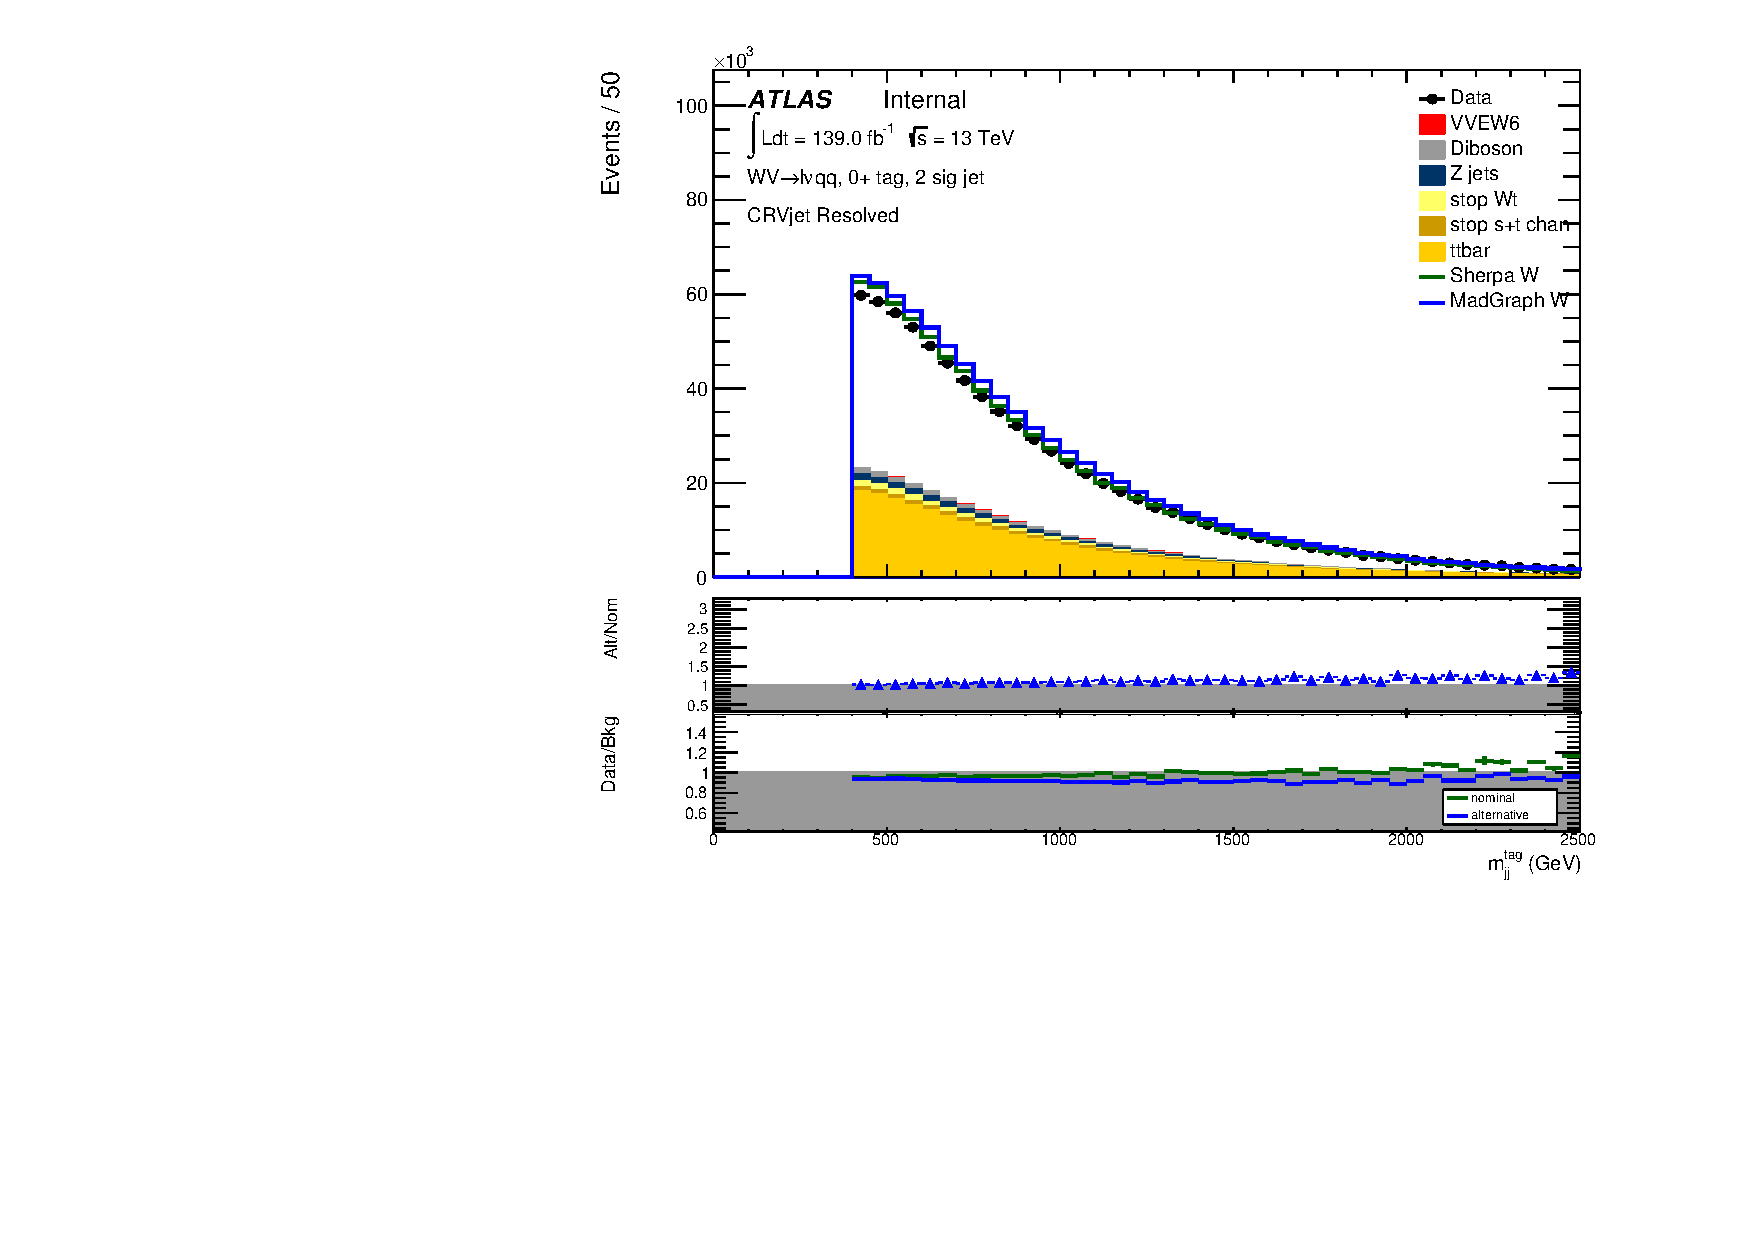
\includegraphics[width=0.3\textwidth]{figures/1lep/ModelUnc/W/C_0ptag2pjet_0ptv_CRVjet_Tight_tagMjj_Lin.pdf}}
	\subfigure[Wjets modelling uncertainties for mjjtag in the Wjets merged control region]{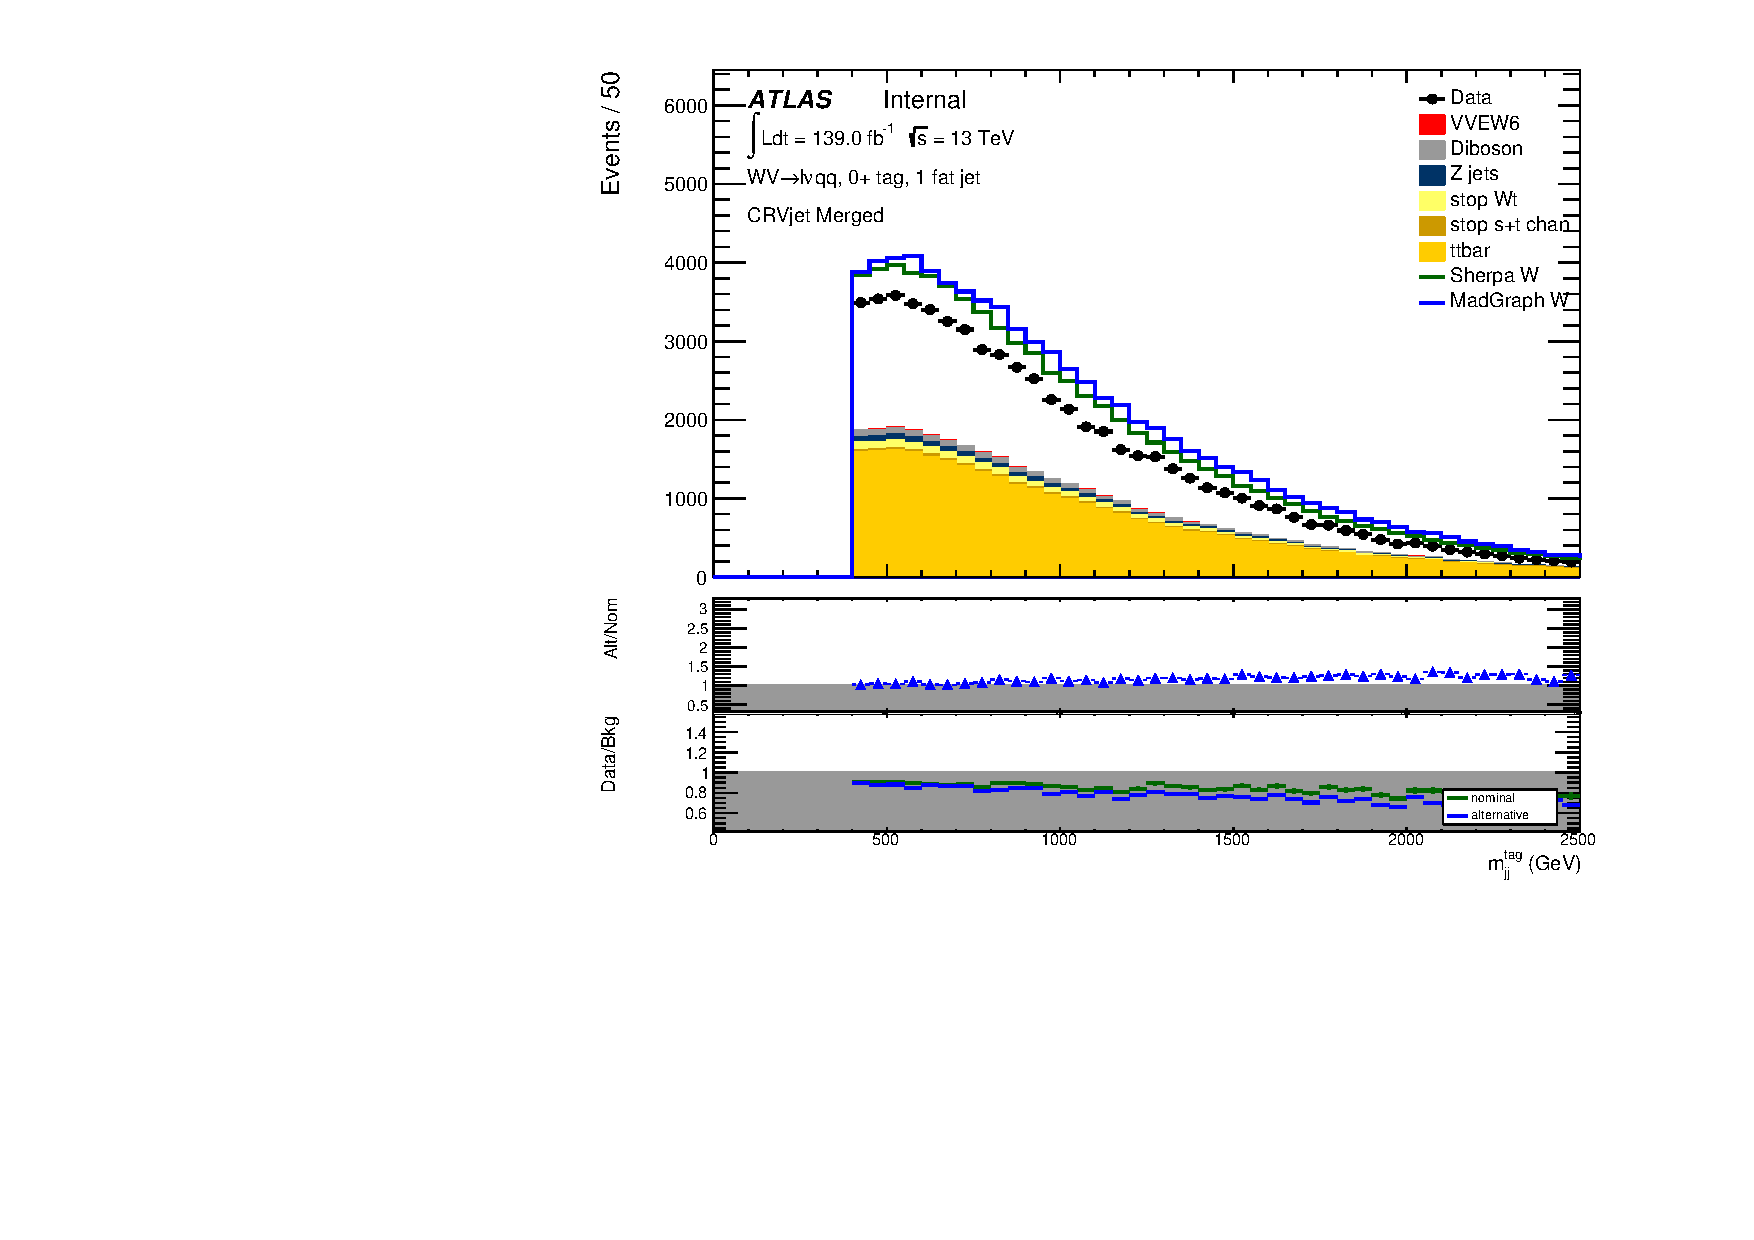
\includegraphics[width=0.3\textwidth]{figures/1lep/ModelUnc/W/C_0ptag1pfat0pjet_0ptv_CRVjet_Merged_tagMjj_Lin.pdf}}\\ 
	\subfigure[Wjets modelling uncertainties for RNN score in the Wjets resolved control region]{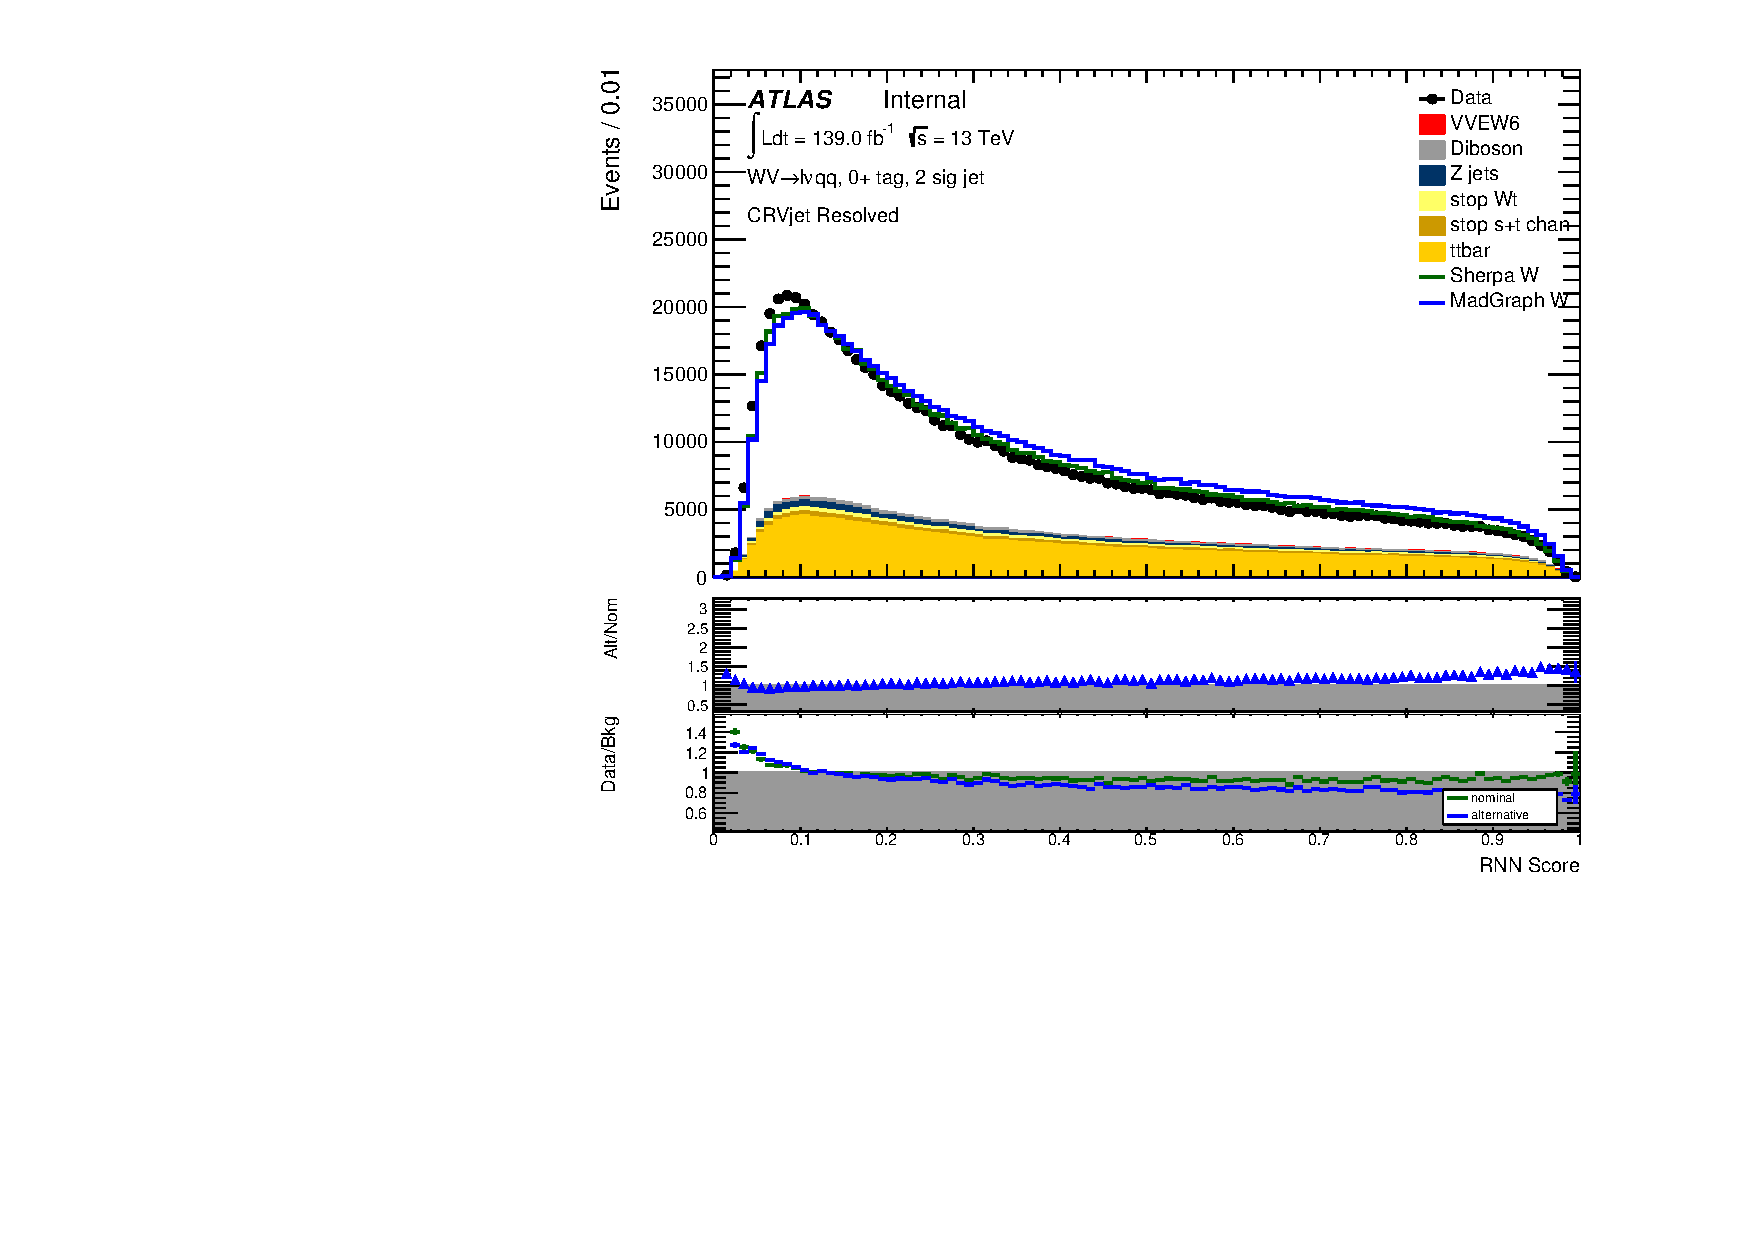
\includegraphics[width=0.3\textwidth]{figures/1lep/ModelUnc/W/C_0ptag2pjet_0ptv_CRVjet_Tight_RNN_Lin.pdf}}
	\subfigure[Wjets modelling uncertainties for RNN score in the Wjets merged control region]{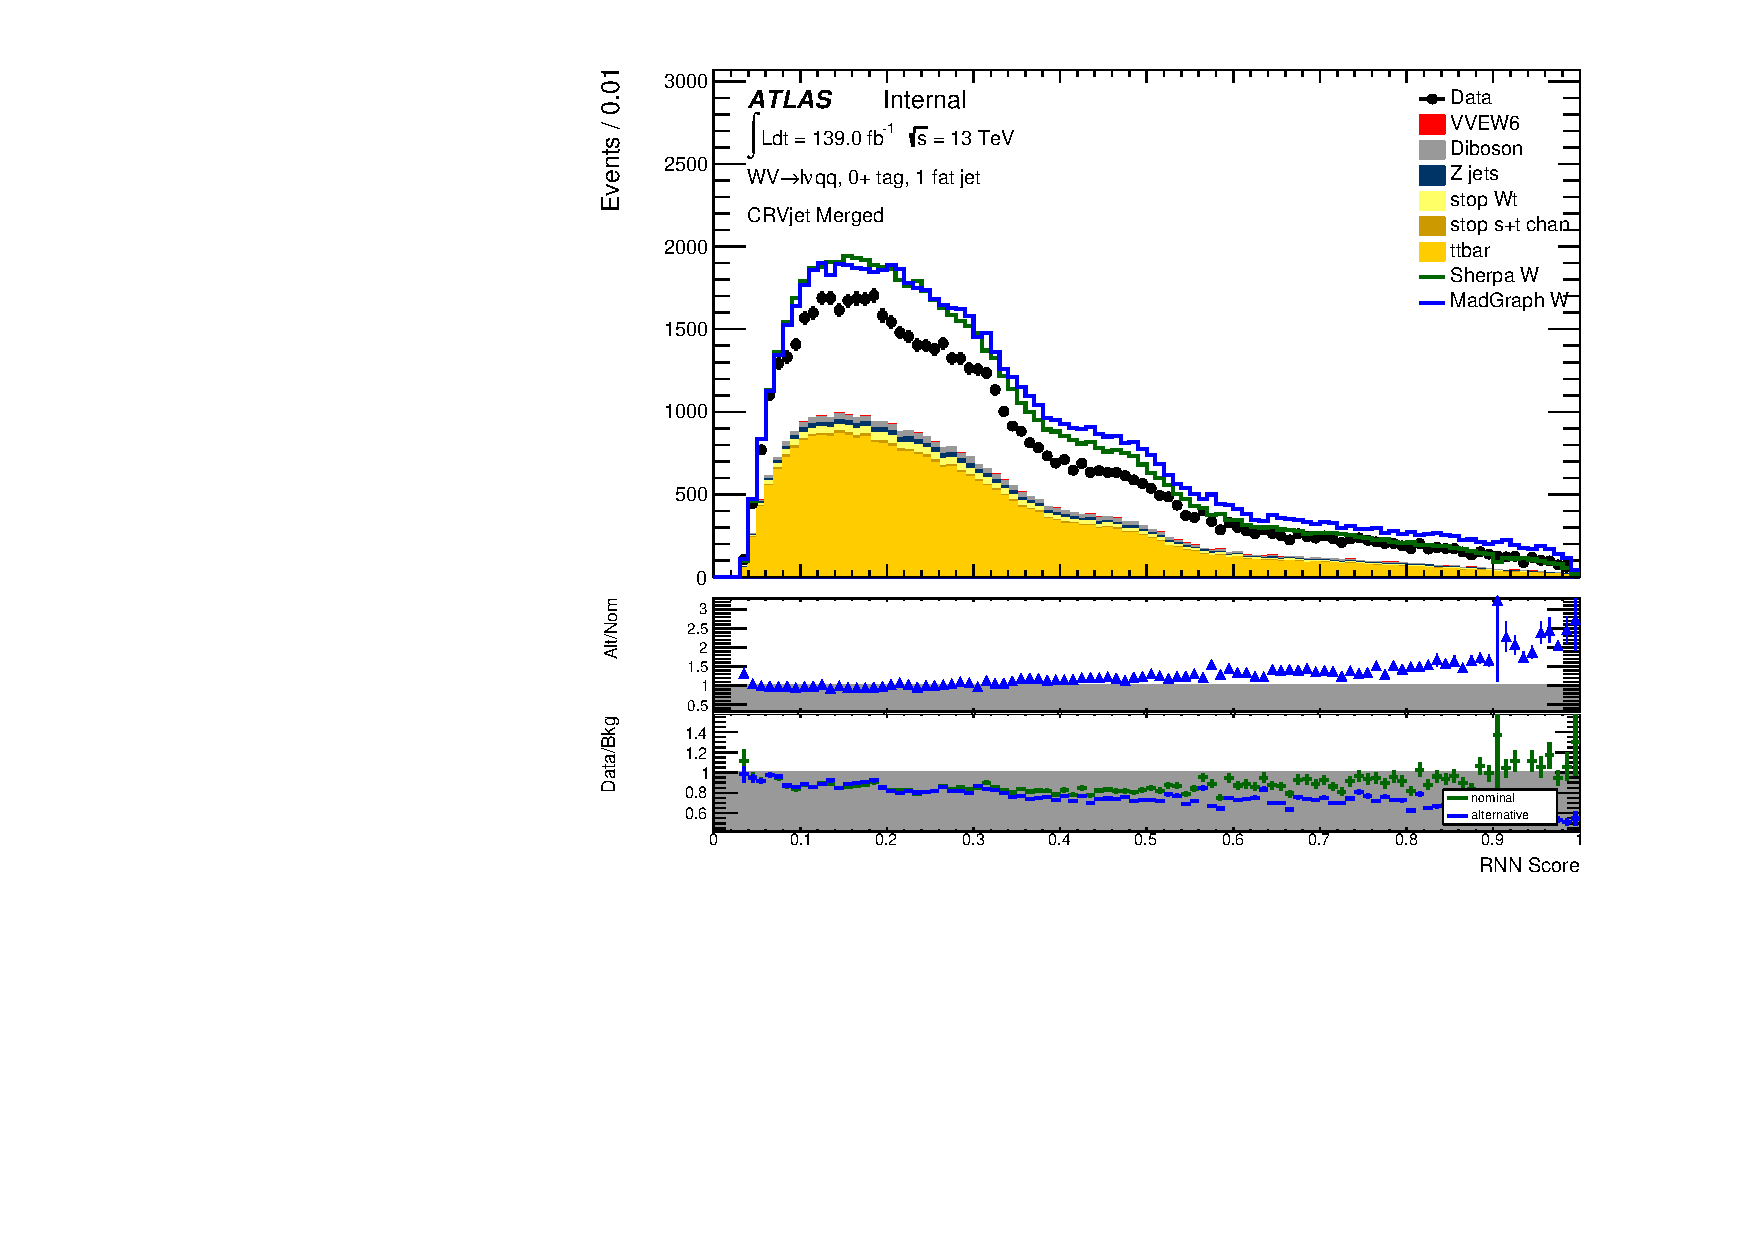
\includegraphics[width=0.3\textwidth]{figures/1lep/ModelUnc/W/C_0ptag1pfat0pjet_0ptv_CRVjet_Merged_RNN_Lin.pdf}}\\
 	\subfigure[Wjets modelling uncertainties for mjjtag in the resolved signal region]{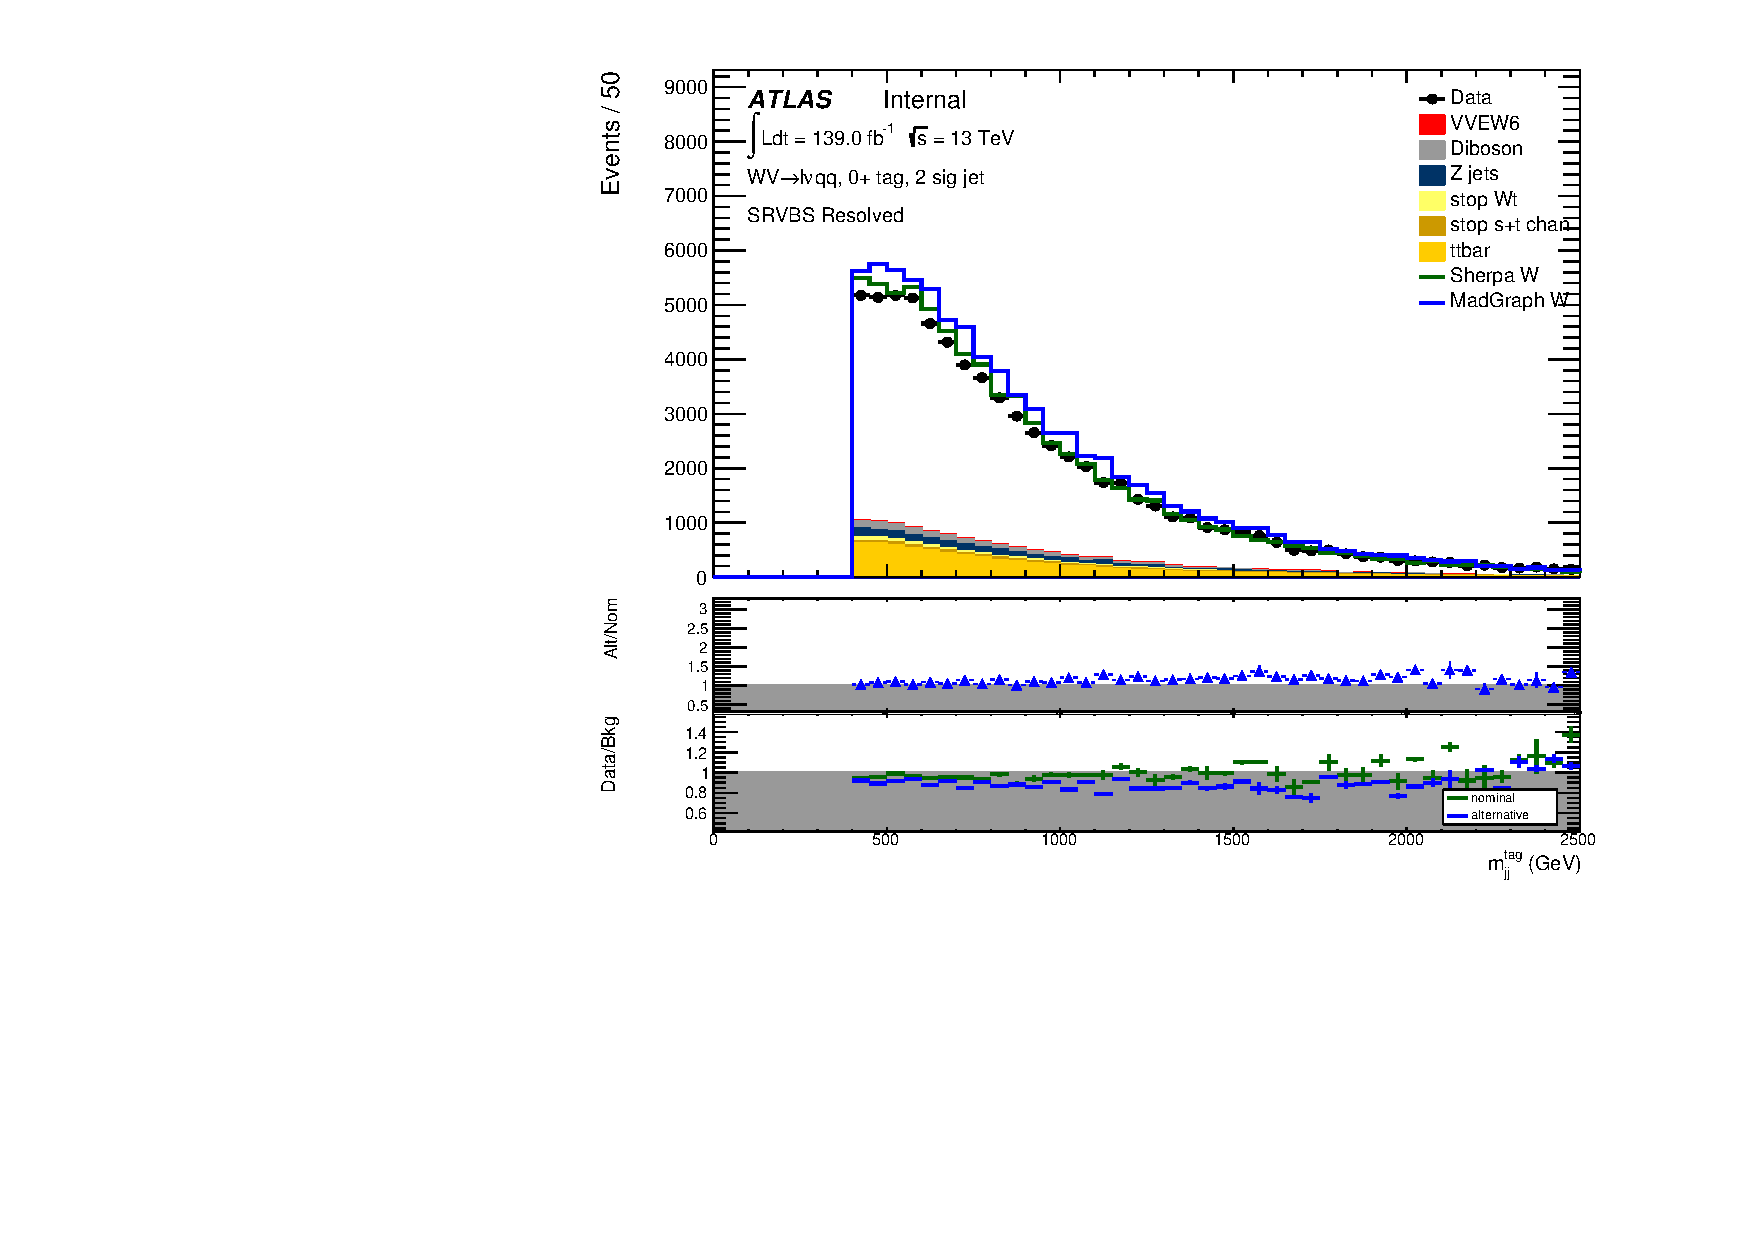
\includegraphics[width=0.3\textwidth]{figures/1lep/ModelUnc/W/C_0ptag2pjet_0ptv_SRVBS_Tight_tagMjj_Lin.pdf}}
        \subfigure[Wjets modelling uncertainties for mjjtag in the merged HP signal region]{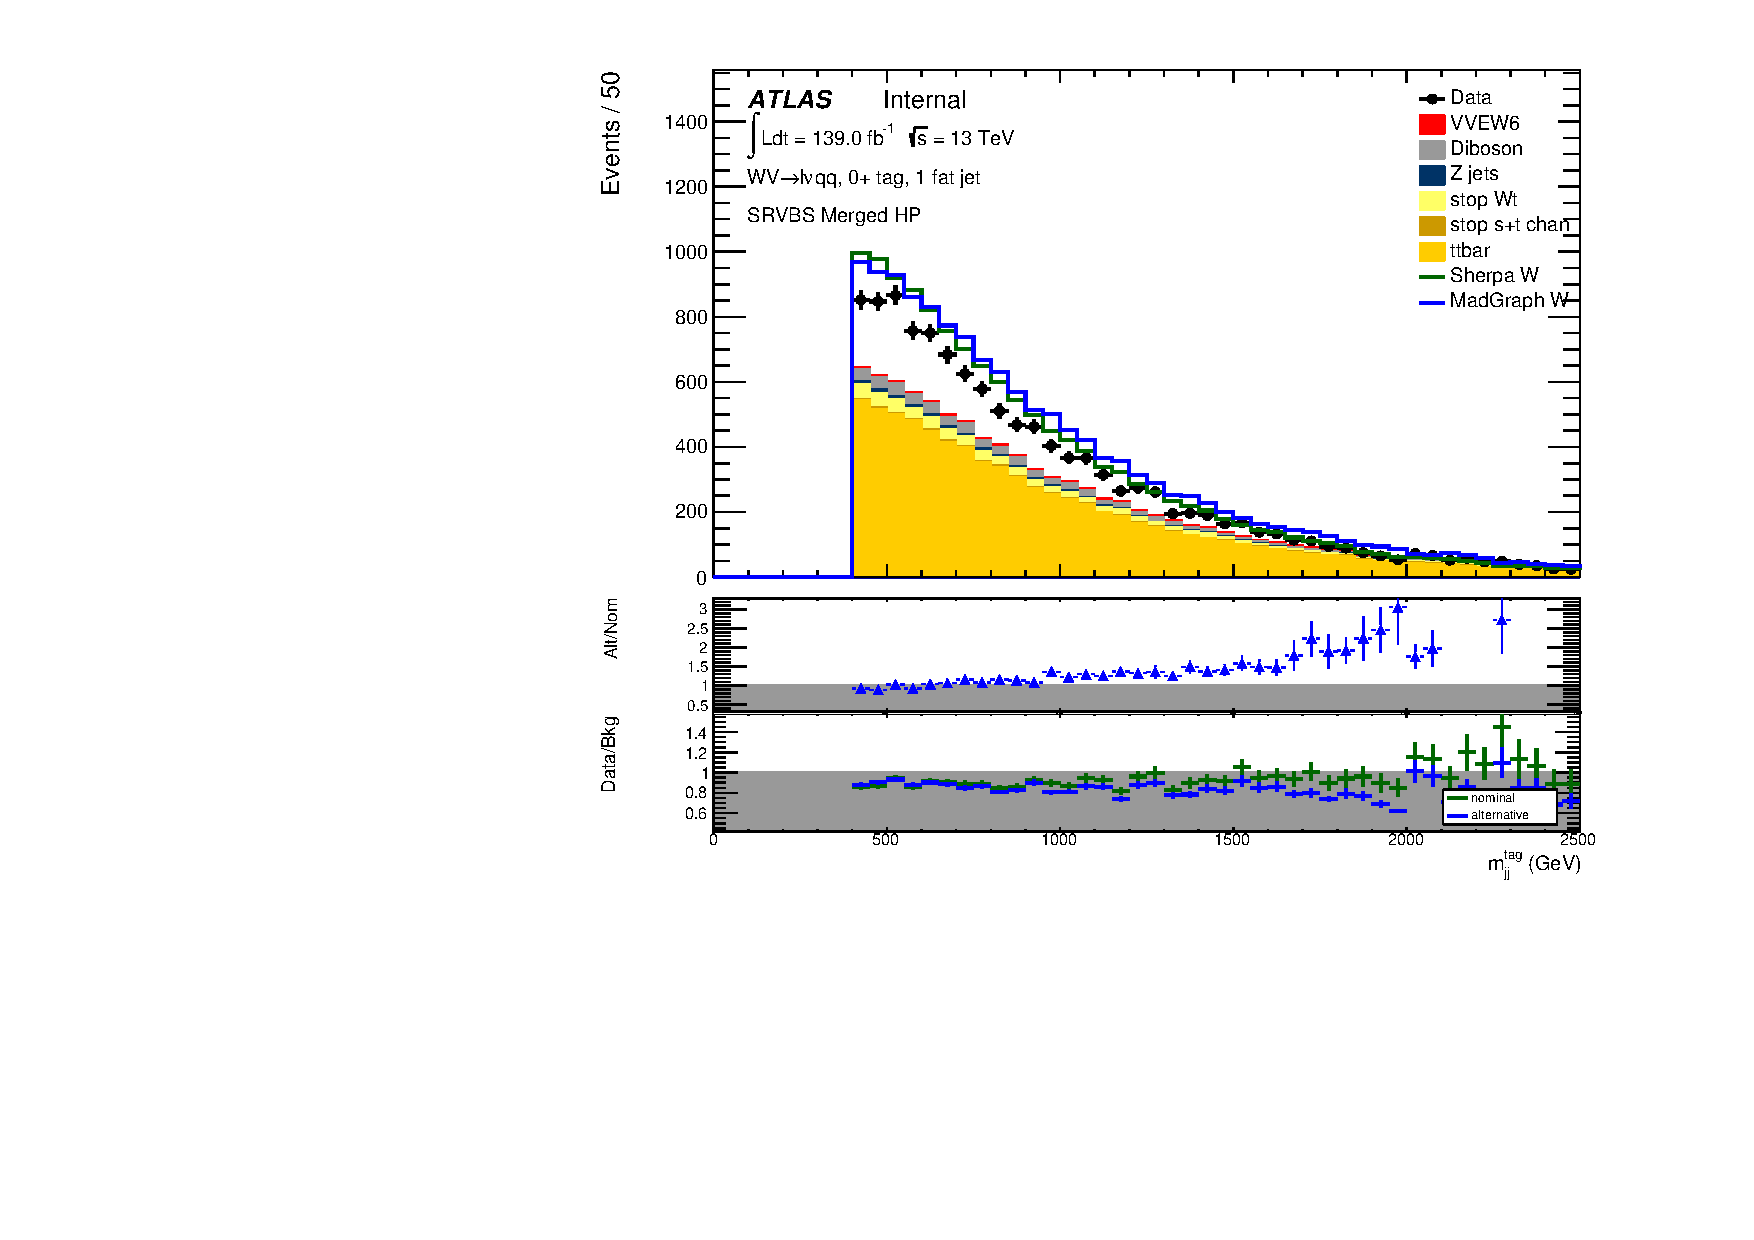
\includegraphics[width=0.3\textwidth]{figures/1lep/ModelUnc/W/C_0ptag1pfat0pjet_0ptv_SRVBS_HP_tagMjj_Lin.pdf}}
        \subfigure[Wjets modelling uncertainties for mjjtag in the merged LP signal region]{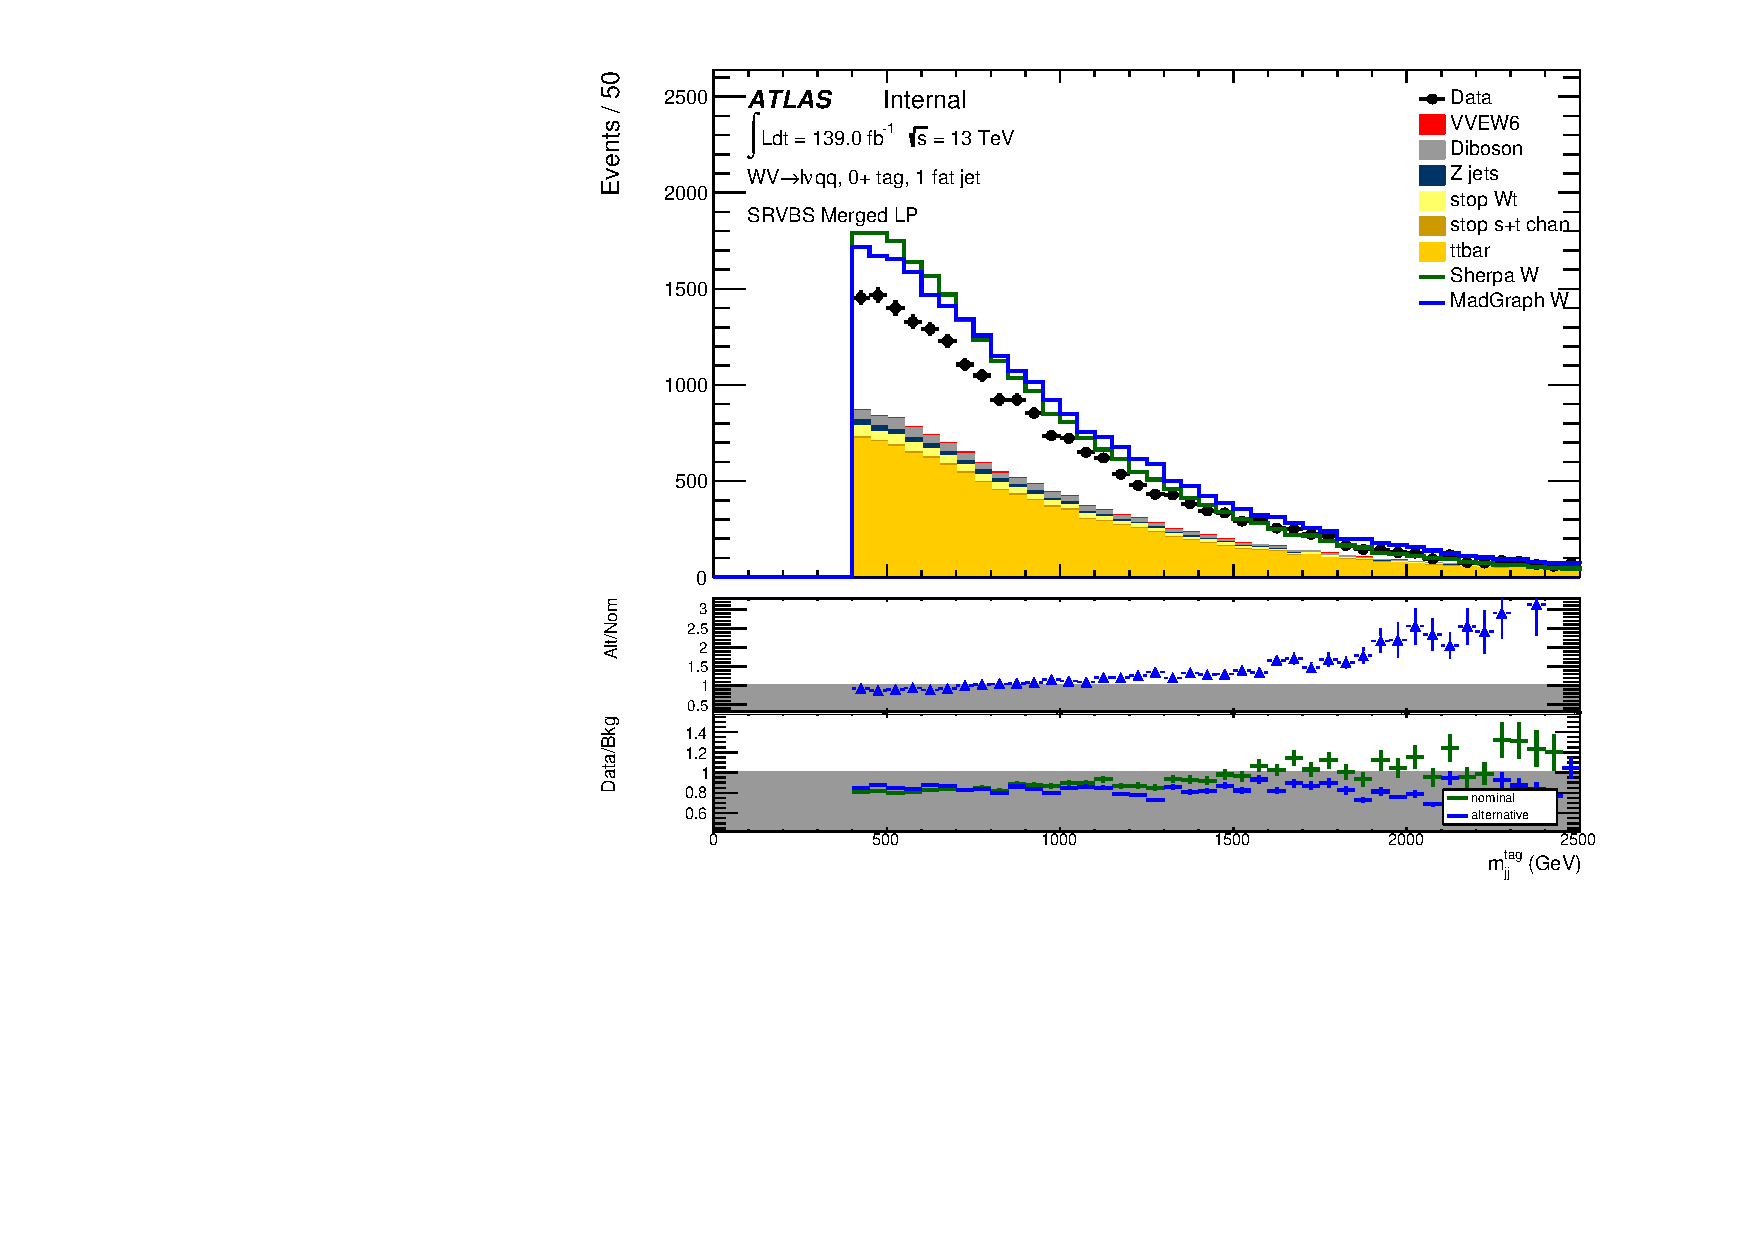
\includegraphics[width=0.3\textwidth]{figures/1lep/ModelUnc/W/C_0ptag1pfat0pjet_0ptv_SRVBS_LP_tagMjj_Lin.pdf}}\\
 	\subfigure[Wjets modelling uncertainties for RNN score in the resolved signal region]{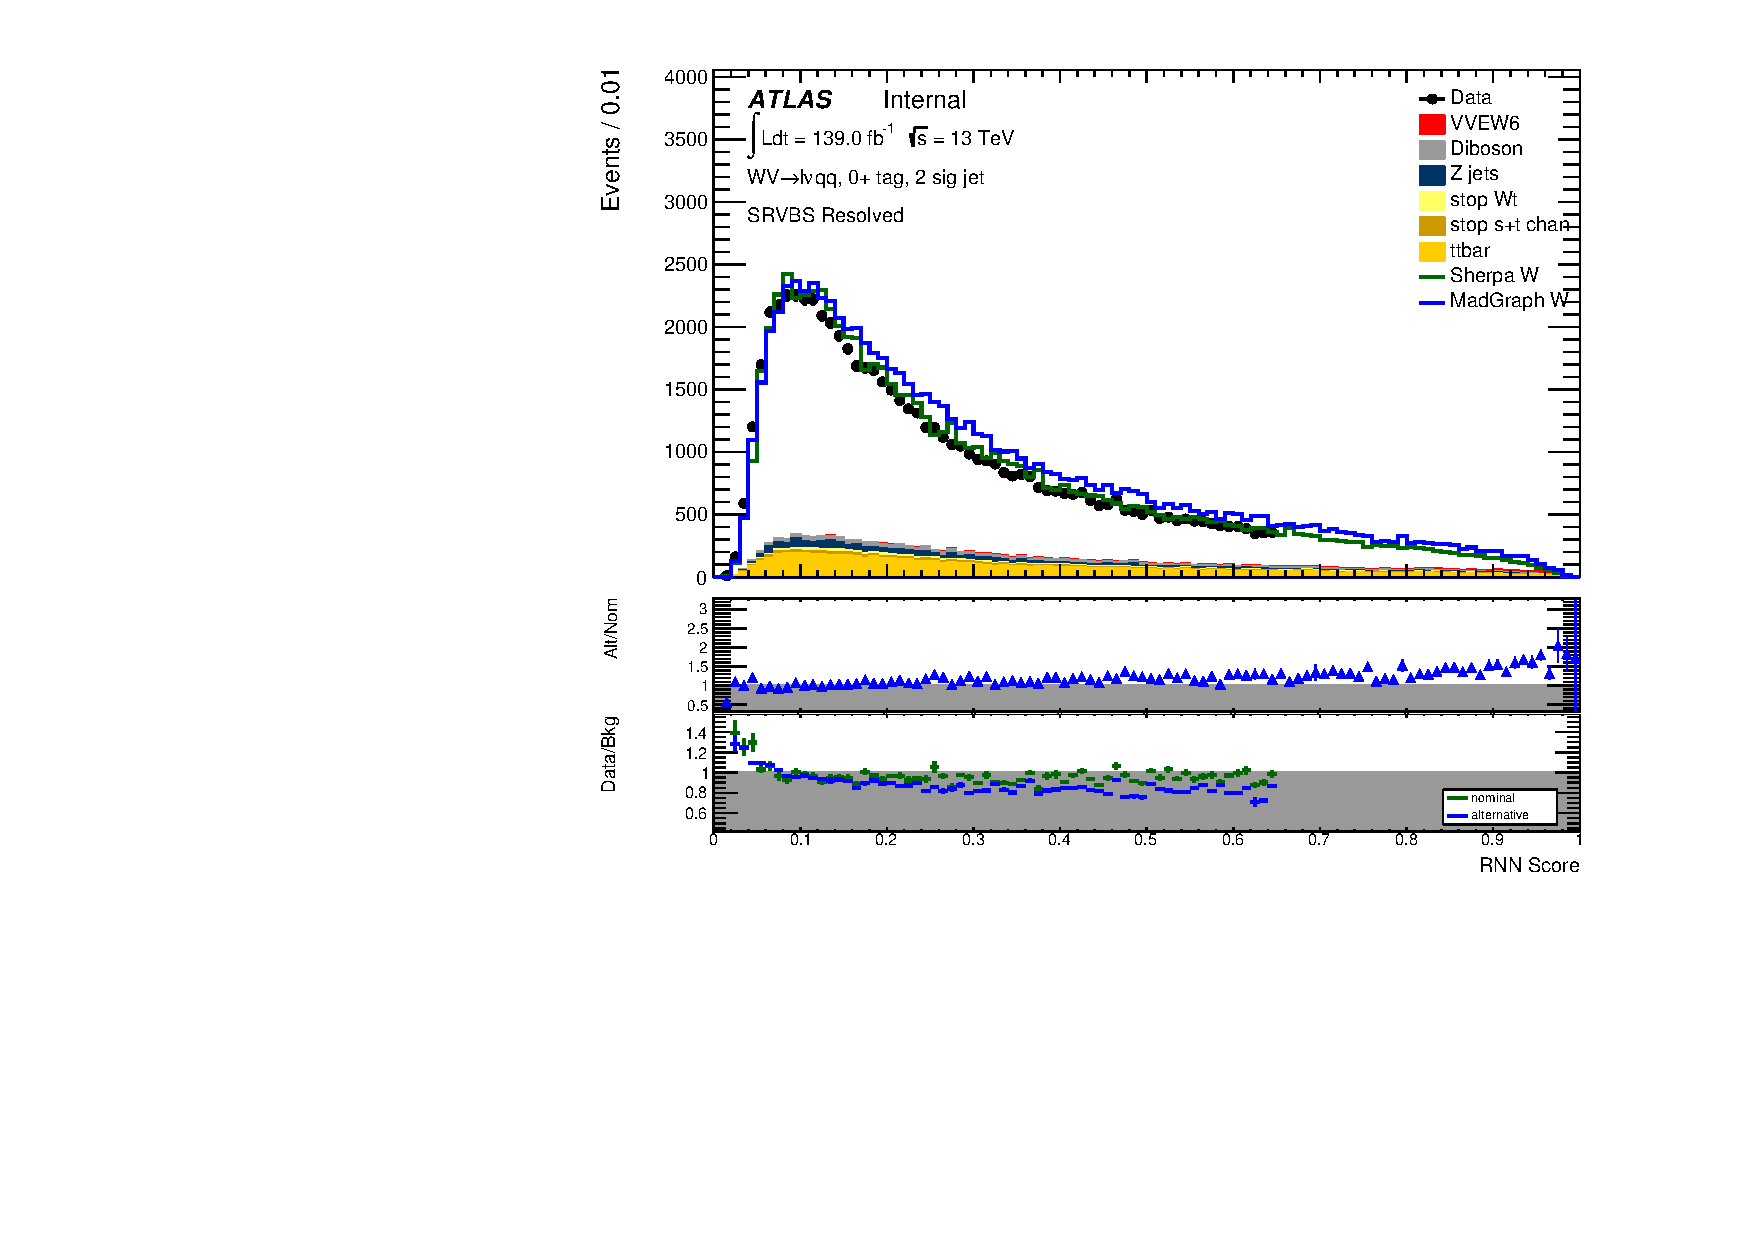
\includegraphics[width=0.3\textwidth]{figures/1lep/ModelUnc/W/C_0ptag2pjet_0ptv_SRVBS_Tight_RNN_Lin.pdf}}
        \subfigure[Wjets modelling uncertainties for RNN score in the merged HP signal region]{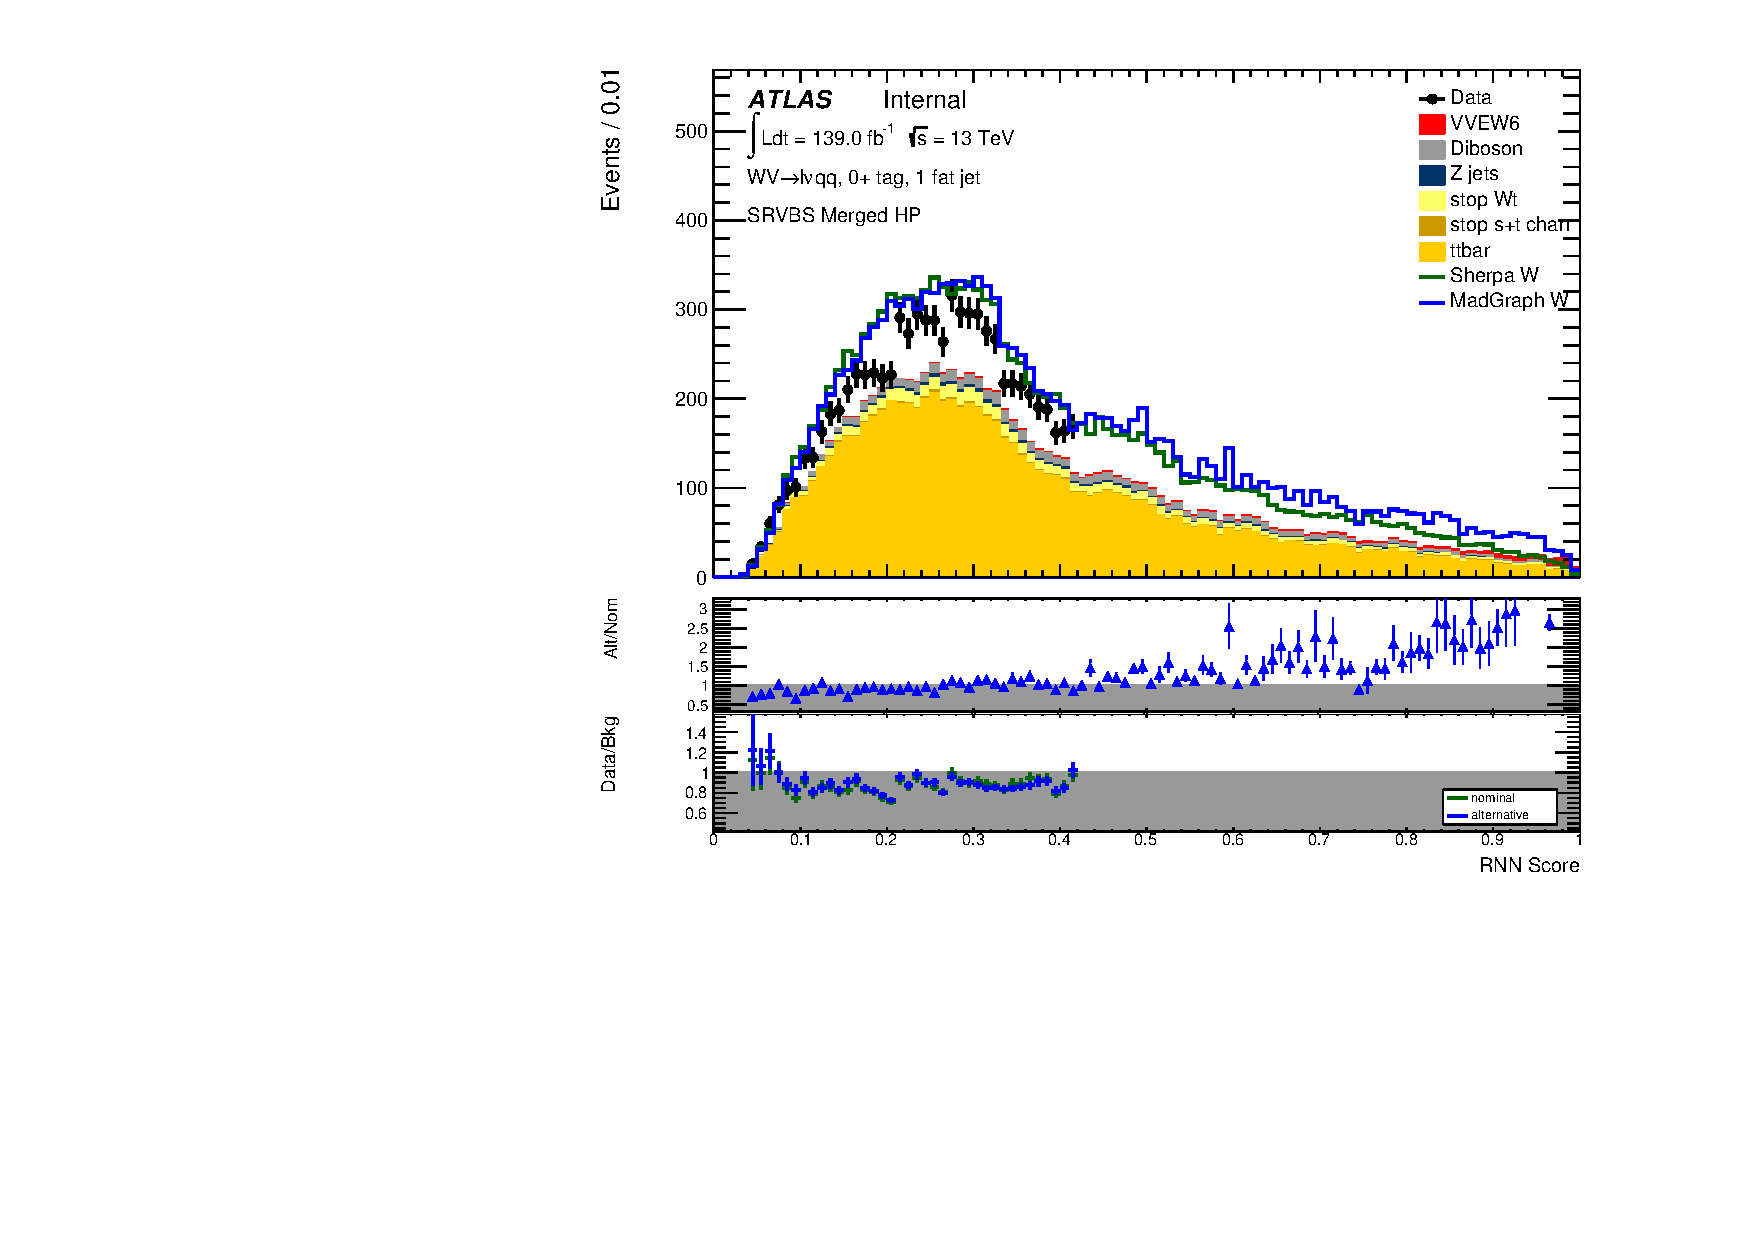
\includegraphics[width=0.3\textwidth]{figures/1lep/ModelUnc/W/C_0ptag1pfat0pjet_0ptv_SRVBS_HP_RNN_Lin.pdf}}
        \subfigure[Wjets modelling uncertainties for RNN score in the merged LP signal region]{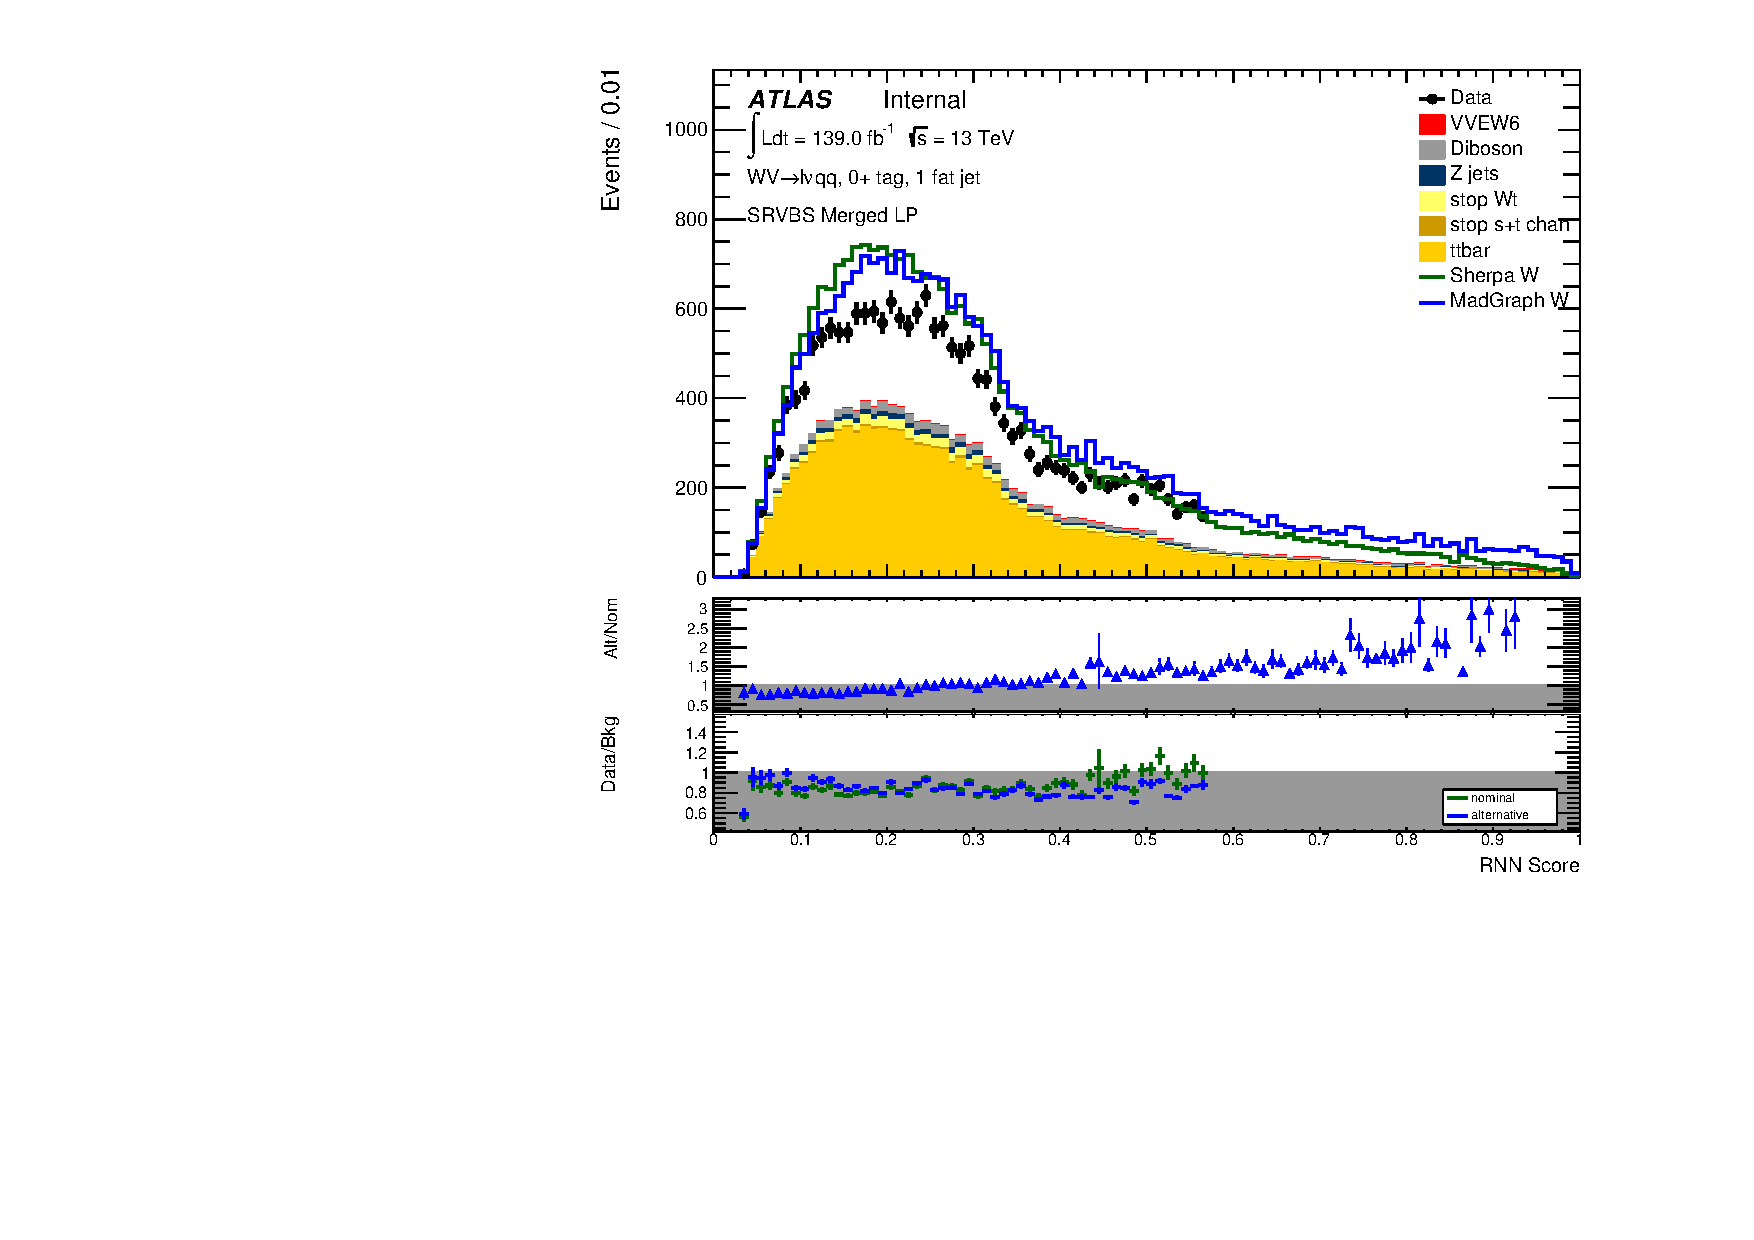
\includegraphics[width=0.3\textwidth]{figures/1lep/ModelUnc/W/C_0ptag1pfat0pjet_0ptv_SRVBS_LP_RNN_Lin.pdf}}
 
        \caption{Modelling uncertainties derived from Sherpa nominal Wjets samples and MadGraph alternative Wjets samples.}
    \label{fig:ModelUncW1Lep}
\end{figure}

%For scale and pdf uncertainties, see \ref{subsec:sig_uncer}.

%%%
\clearpage
\subsubsection{Top: alternative samples}
\label{subsec:bkg_uncer_top}

Figures
\ref{fig:ModelUncttbar0Lep}
show the comparison of the nominal ttbar sample with the alternative samples.

\begin{figure}[ht]
    \centering
        \subfigure[HP SR: jet multiplicity]{\includegraphics[width=0.3\textwidth]{figures/0lep/final-mvaInputs/merged/plots/comparisonaltovernom_PowhegHerwig_recojN_SRVBS_HP}}
        \subfigure[LP SR: jet multiplicity]{\includegraphics[width=0.3\textwidth]{figures/0lep/final-mvaInputs/merged/plots/comparisonaltovernom_PowhegHerwig_recojN_SRVBS_LP}}
        \subfigure[resolved SR: jet multiplicity]{\includegraphics[width=0.3\textwidth]{figures/0lep/final-mvaInputs/merged/plots/comparisonaltovernom_PowhegHerwig_recojN_SRVBS_Fid}}\\
        \subfigure[HP SR: RNN score]{\includegraphics[width=0.3\textwidth]{figures/0lep/final-fullSyst/merged/plots/comparisonaltovernom_PowhegHerwig_RNN_SRVBS_HP}}
        \subfigure[LP SR: RNN score]{\includegraphics[width=0.3\textwidth]{figures/0lep/final-fullSyst/merged/plots/comparisonaltovernom_PowhegHerwig_RNN_SRVBS_LP}}
        \subfigure[resolved SR: RNN score]{\includegraphics[width=0.3\textwidth]{figures/0lep/final-fullSyst/merged/plots/comparisonaltovernom_PowhegHerwig_RNN_SRVBS_Fid}}\\
        \subfigure[HP SR: NN score]{\includegraphics[width=0.3\textwidth]{figures/0lep/final-fullSyst/merged/plots/comparisonaltovernom_PowhegHerwig_NN_SRVBS_HP}}
        \subfigure[LP SR: NN score]{\includegraphics[width=0.3\textwidth]{figures/0lep/final-fullSyst/merged/plots/comparisonaltovernom_PowhegHerwig_NN_SRVBS_LP}}
        \subfigure[resolved SR: NN score]{\includegraphics[width=0.3\textwidth]{figures/0lep/final-fullSyst/merged/plots/comparisonaltovernom_PowhegHerwig_NN_SRVBS_Fid}}\\
%       \subfigure[merged CR: tag jet system mass]{\includegraphics[width=0.3\textwidth]{figures/0lep/final-mvaInputs/merged/plots/comparisonaltovernom_PowhegHerwig_MTagJets_CRVjet_Mer}}                                                                                                                                                                       
%       \subfigure[resolved CR: tag jet system mass]{\includegraphics[width=0.3\textwidth]{figures/0lep/final-mvaInputs/merged/plots/comparisonaltovernom_PowhegHerwig_MTagJets_CRVjet_Fid}}                                                                                                                                                                       
        \caption{Modelling differences between PowhegPythia nominal ttbar samples and PowhegHerwig alternative ttbar samples in the  0-lepton channel.}
    \label{fig:ModelUncttbar0Lep}
\end{figure}


\begin{figure}[ht]
    \centering
	\subfigure[ttbar shower uncertainties for mjjtag in the resolved top control region]{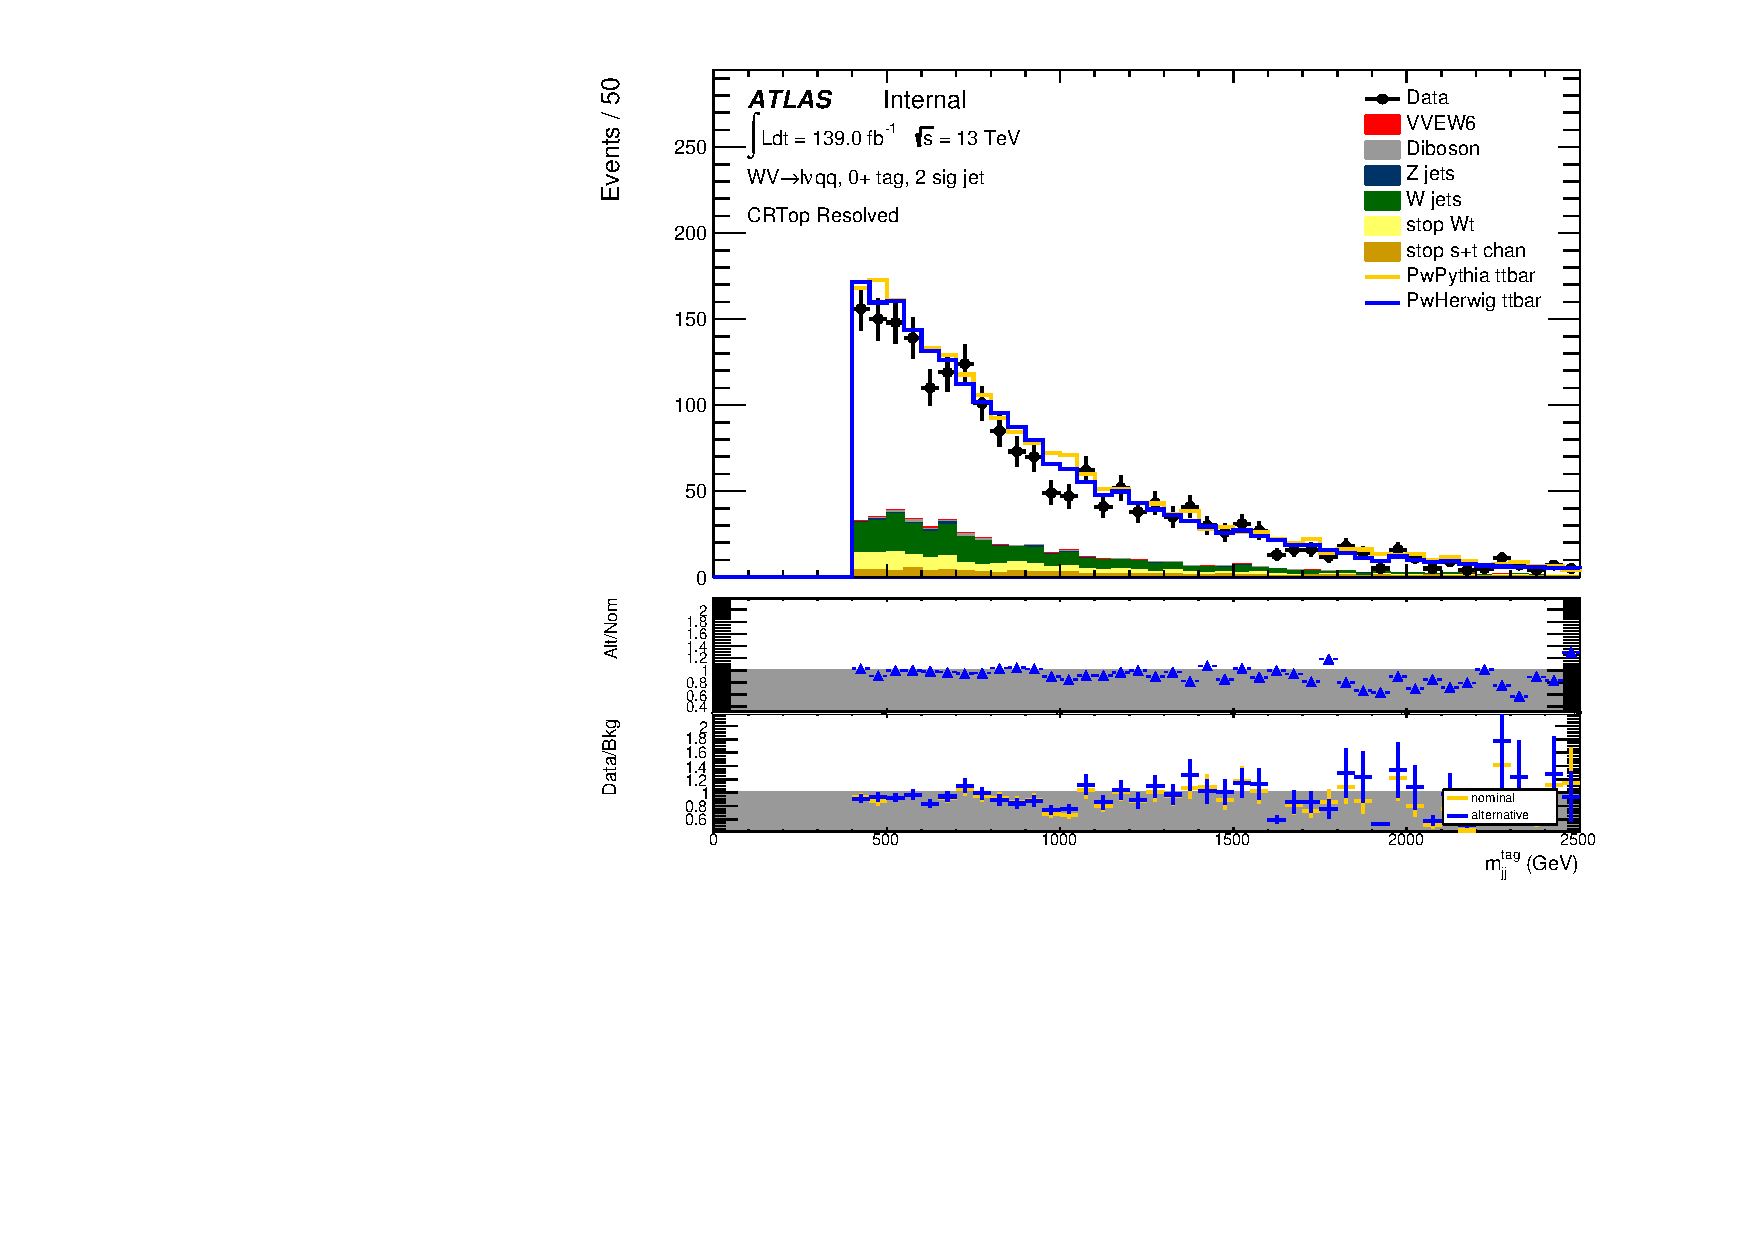
\includegraphics[width=0.3\textwidth]{figures/1lep/ModelUnc/ttbarPwHg/C_0ptag2pjet_0ptv_CRTop_Tight_tagMjj_Lin.pdf}}
        \subfigure[ttbar shower uncertainties for mjjtag in the merged HP top control region]{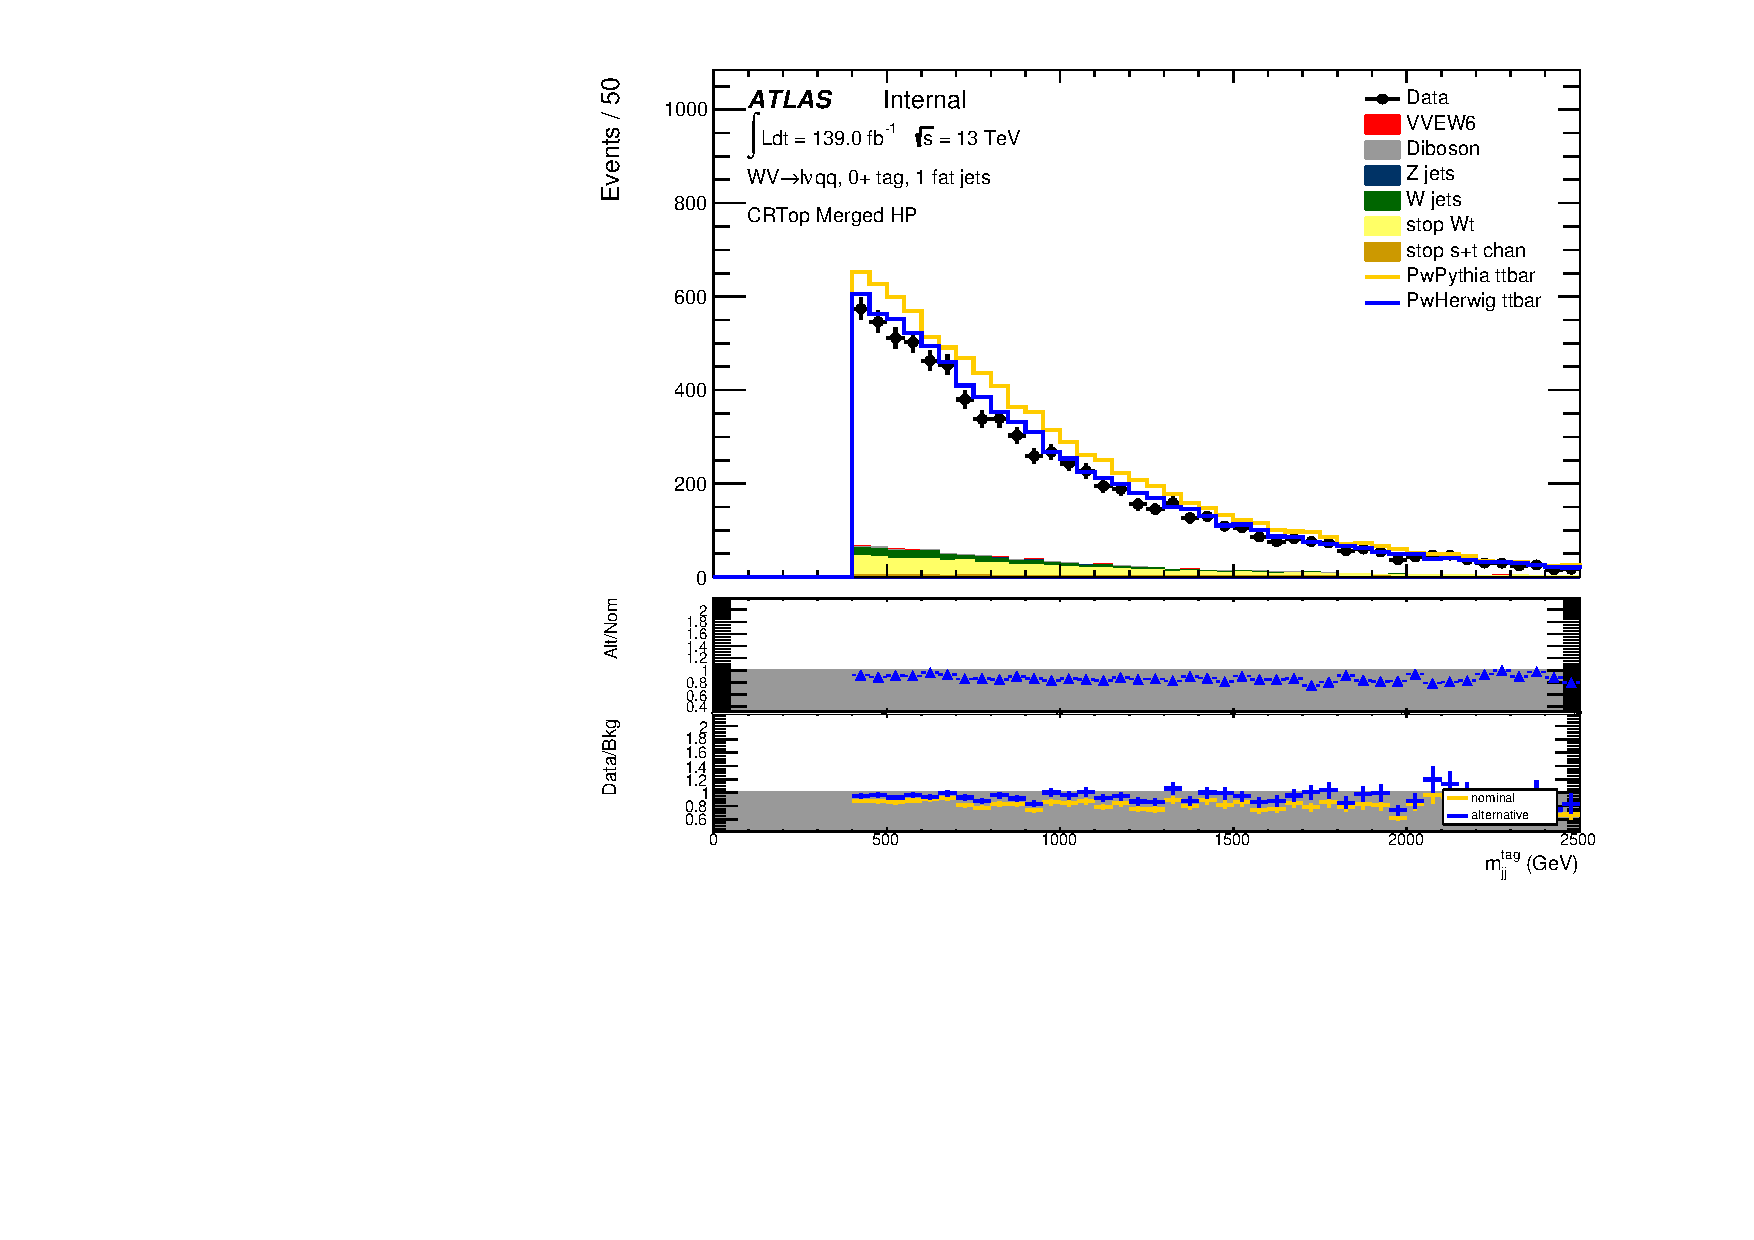
\includegraphics[width=0.3\textwidth]{figures/1lep/ModelUnc/ttbarPwHg/C_0ptag1pfat0pjet_0ptv_CRTop_HP_tagMjj_Lin.pdf}}
        \subfigure[ttbar shower uncertainties for mjjtag in the merged LP top control region]{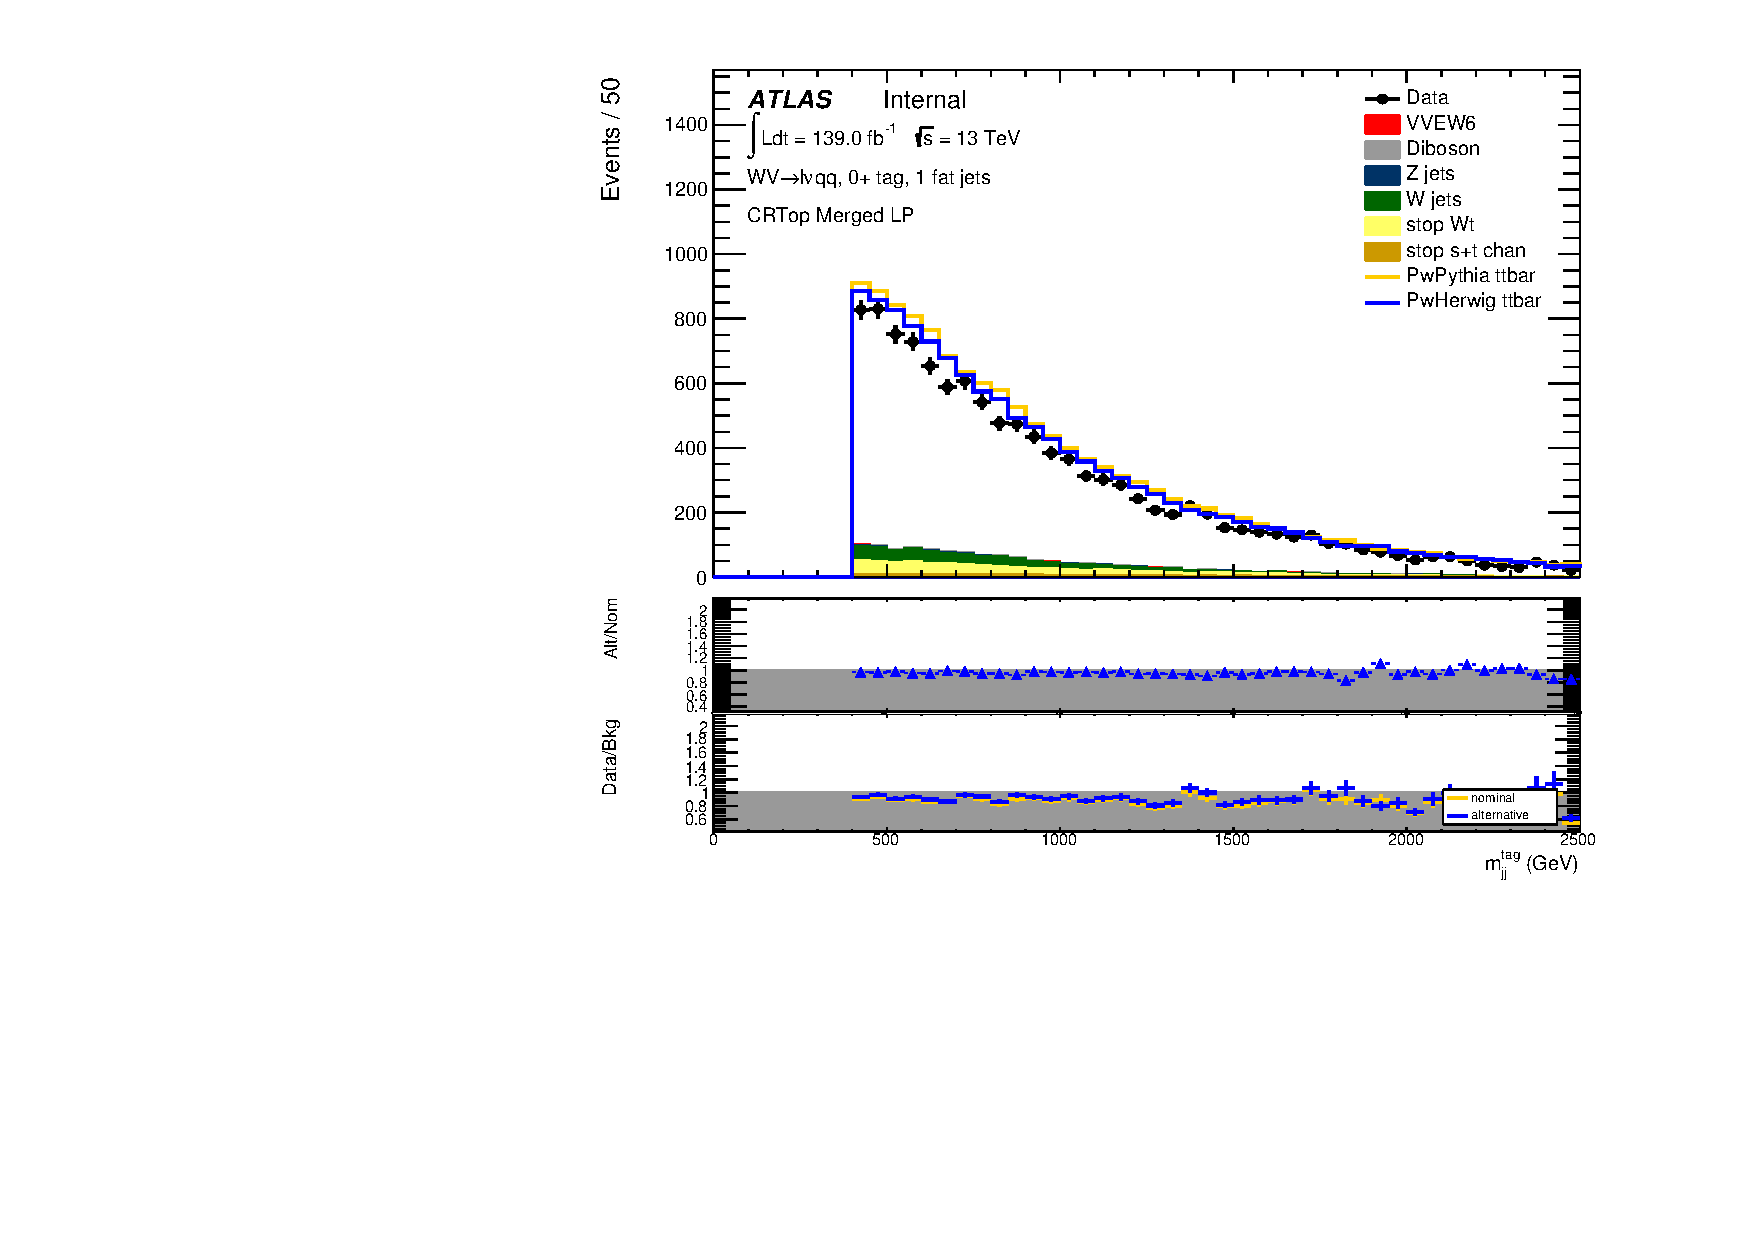
\includegraphics[width=0.3\textwidth]{figures/1lep/ModelUnc/ttbarPwHg/C_0ptag1pfat0pjet_0ptv_CRTop_LP_tagMjj_Lin.pdf}}\\
        \subfigure[ttbar shower uncertainties for RNN score in the resolved top control region]{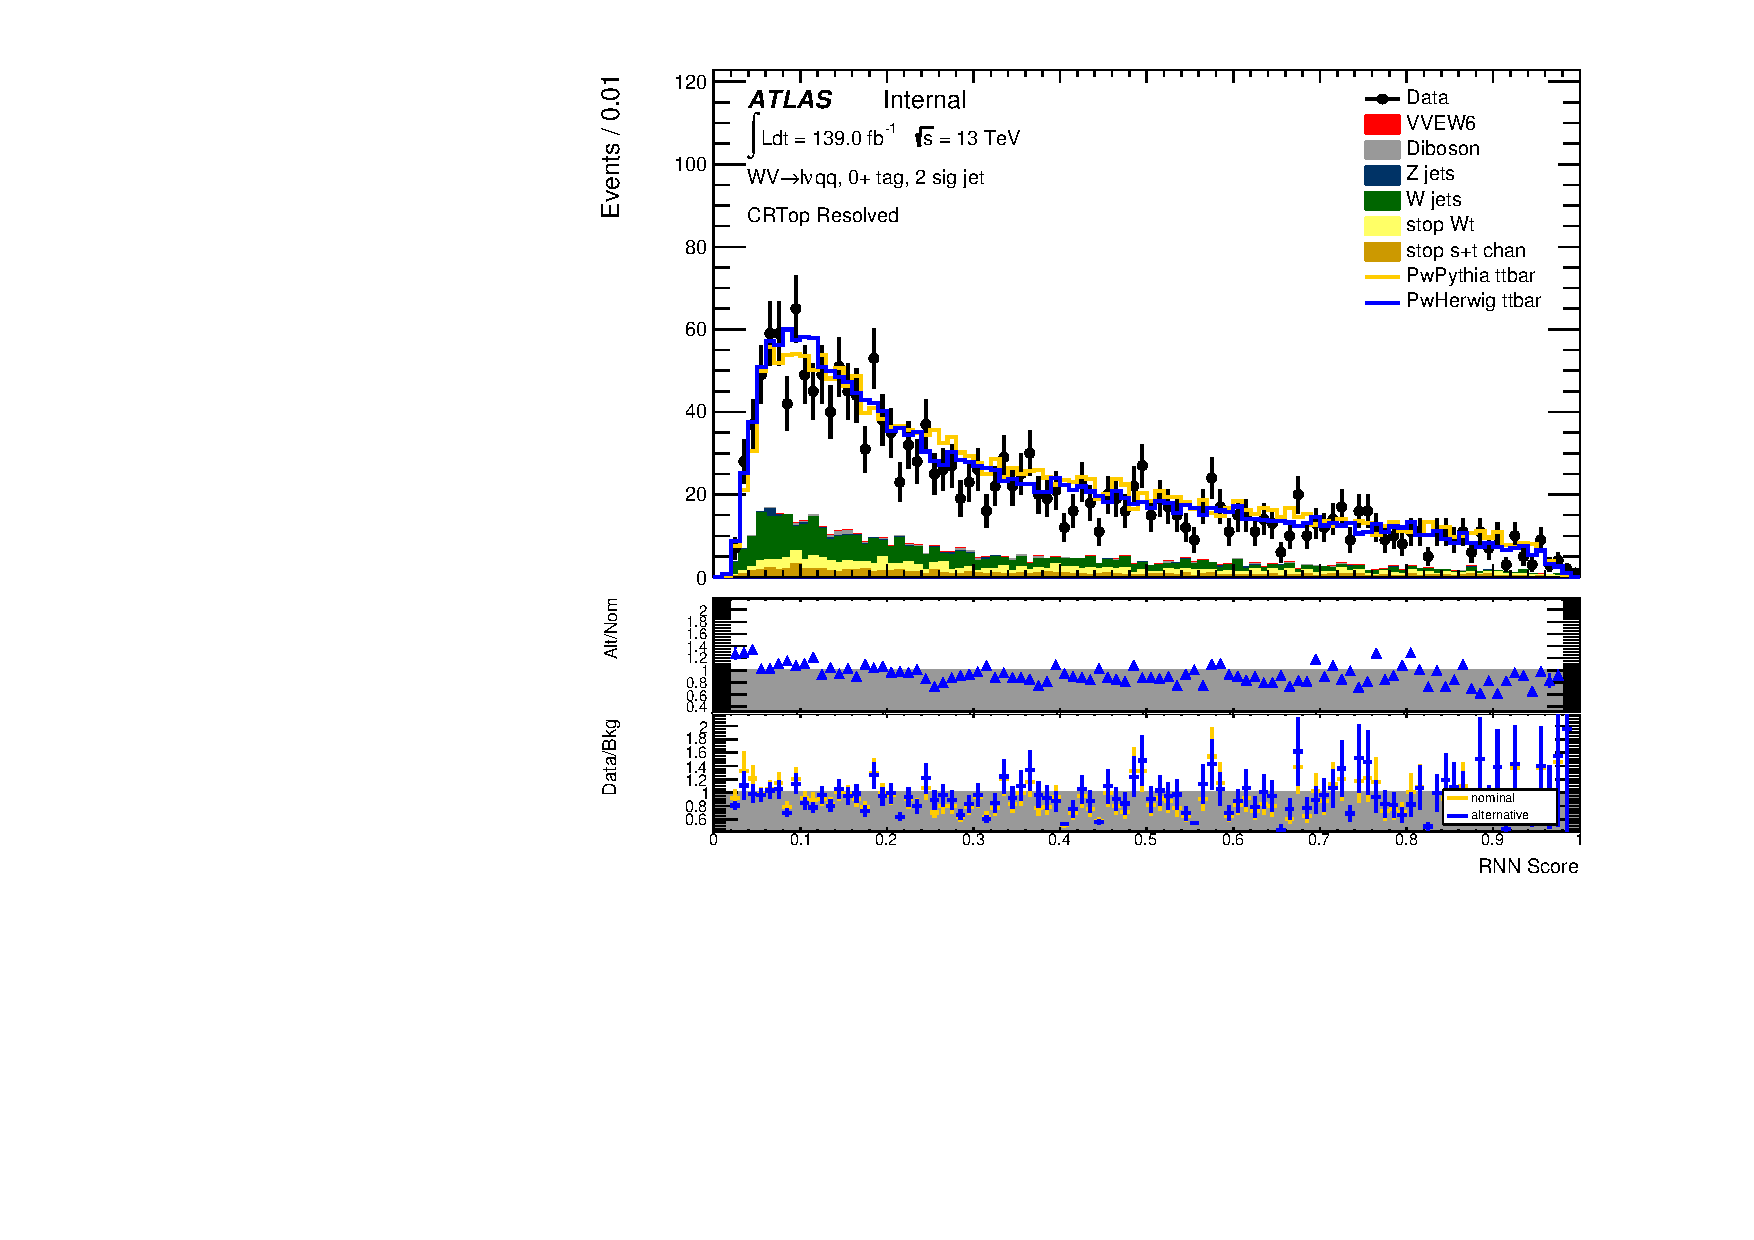
\includegraphics[width=0.3\textwidth]{figures/1lep/ModelUnc/ttbarPwHg/C_0ptag2pjet_0ptv_CRTop_Tight_RNN_Lin.pdf}}
        \subfigure[ttbar shower uncertainties for RNN score in the merged HP top control region]{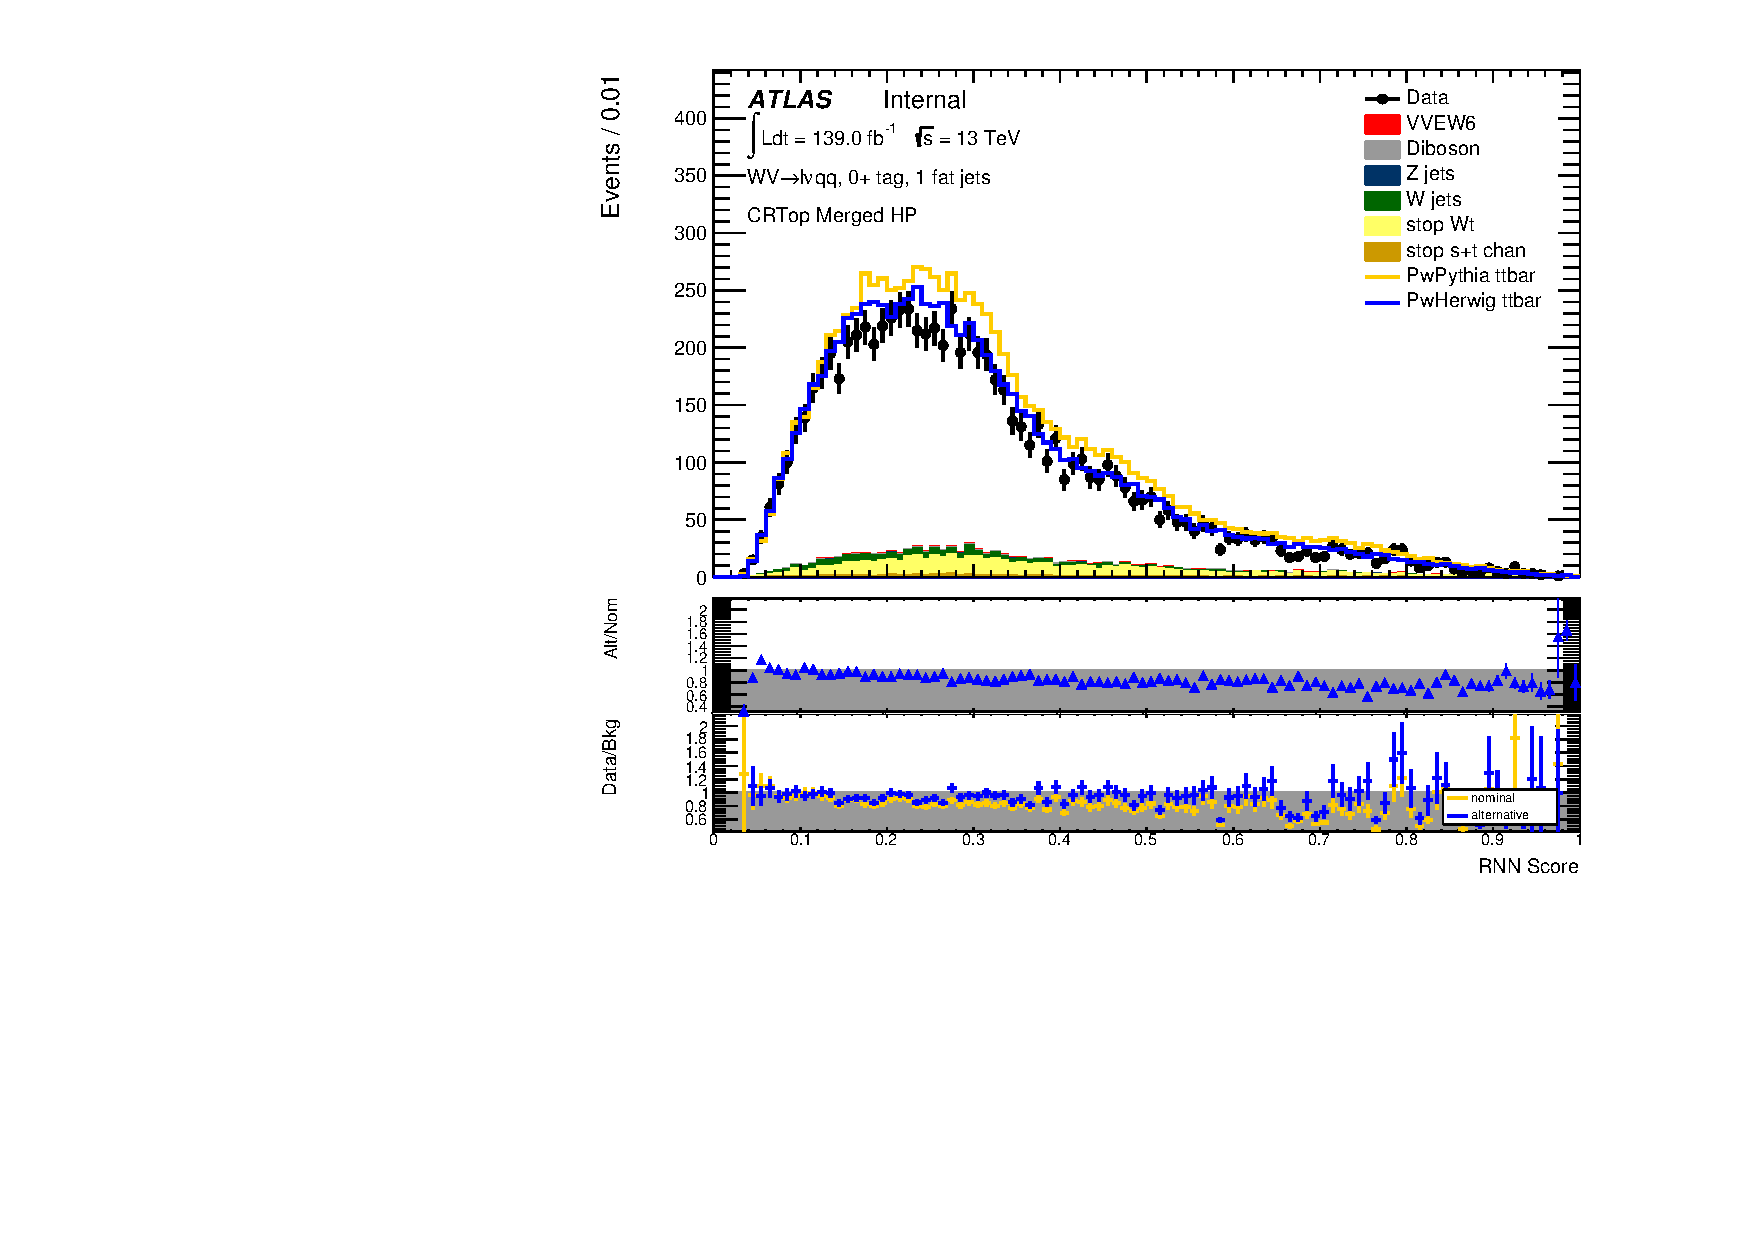
\includegraphics[width=0.3\textwidth]{figures/1lep/ModelUnc/ttbarPwHg/C_0ptag1pfat0pjet_0ptv_CRTop_HP_RNN_Lin.pdf}}
        \subfigure[ttbar shower uncertainties for RNN score in the merged LP top control region]{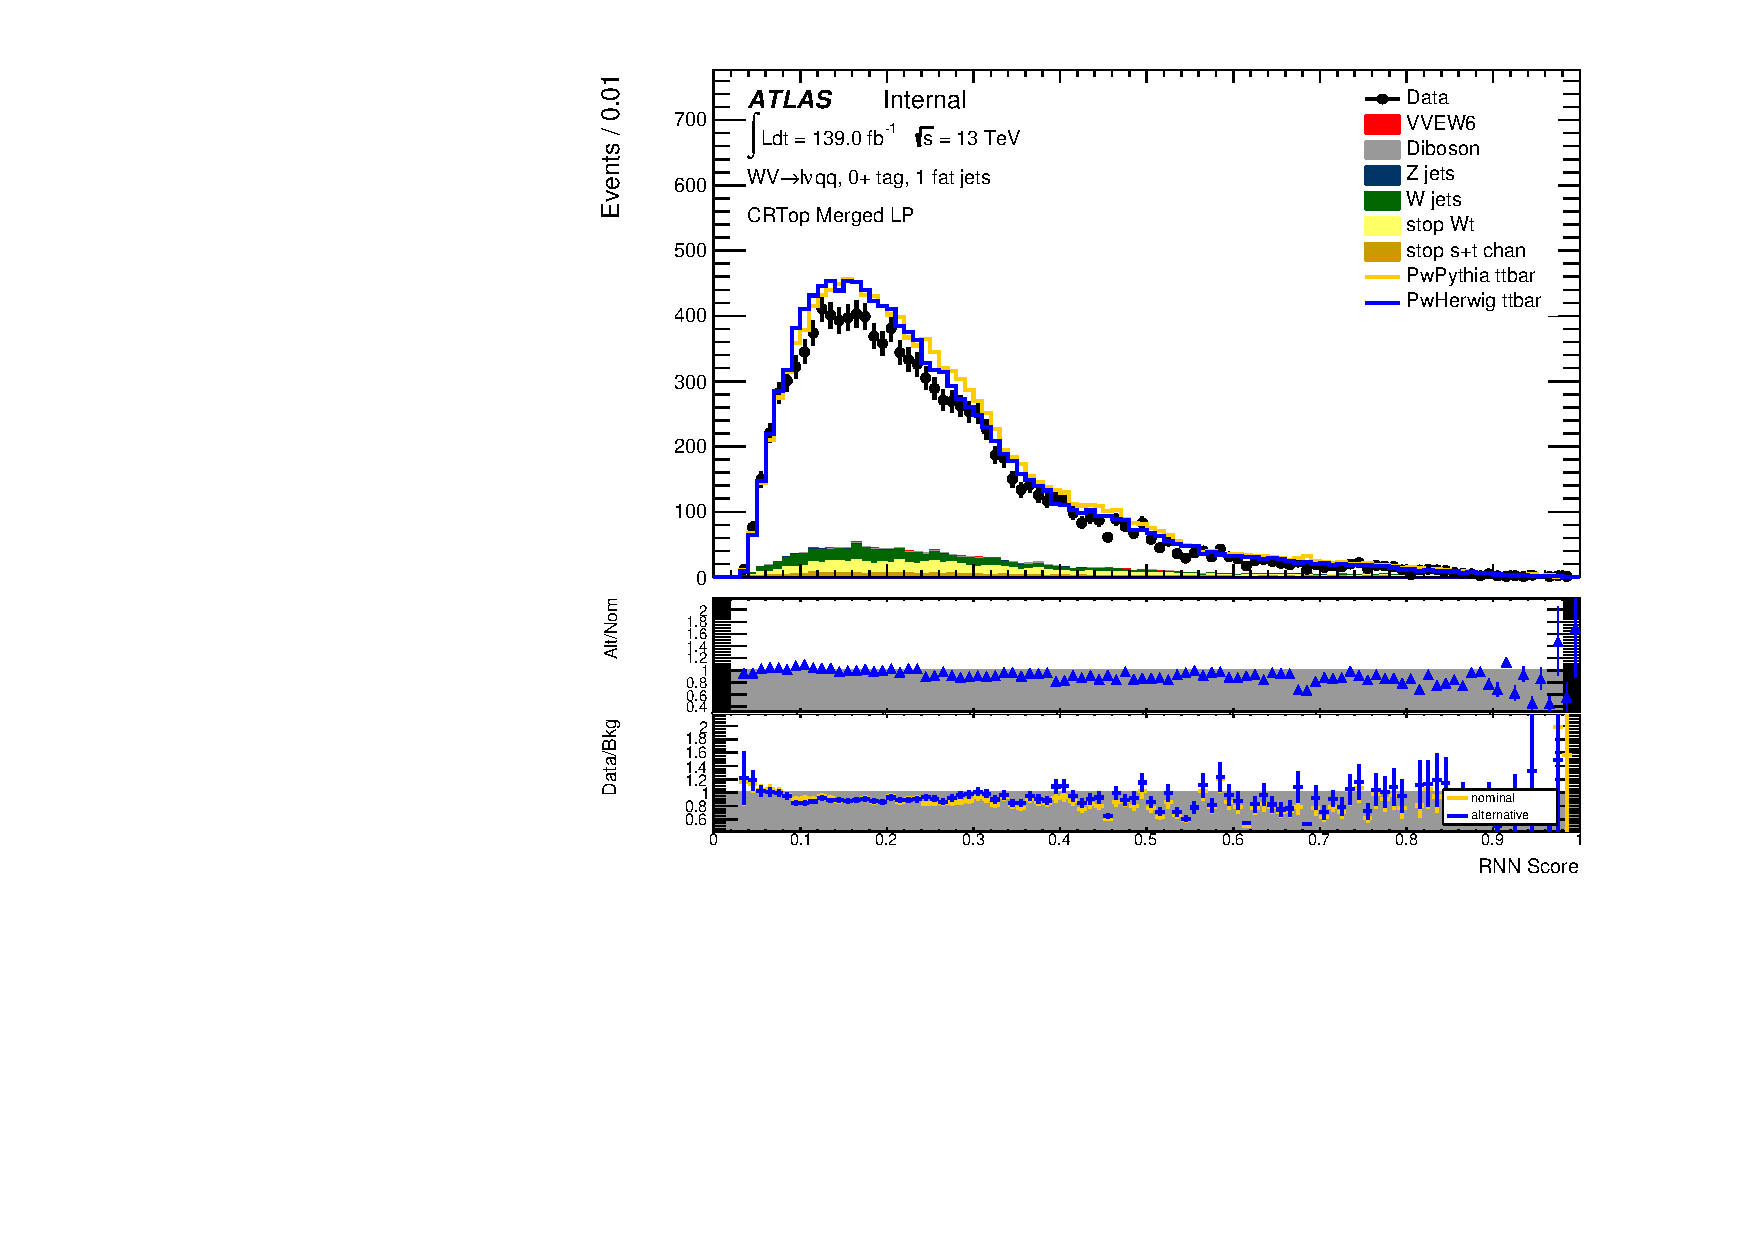
\includegraphics[width=0.3\textwidth]{figures/1lep/ModelUnc/ttbarPwHg/C_0ptag1pfat0pjet_0ptv_CRTop_LP_RNN_Lin.pdf}}\\
        \subfigure[ttbar shower uncertainties for mjjtag in the resolved signal region]{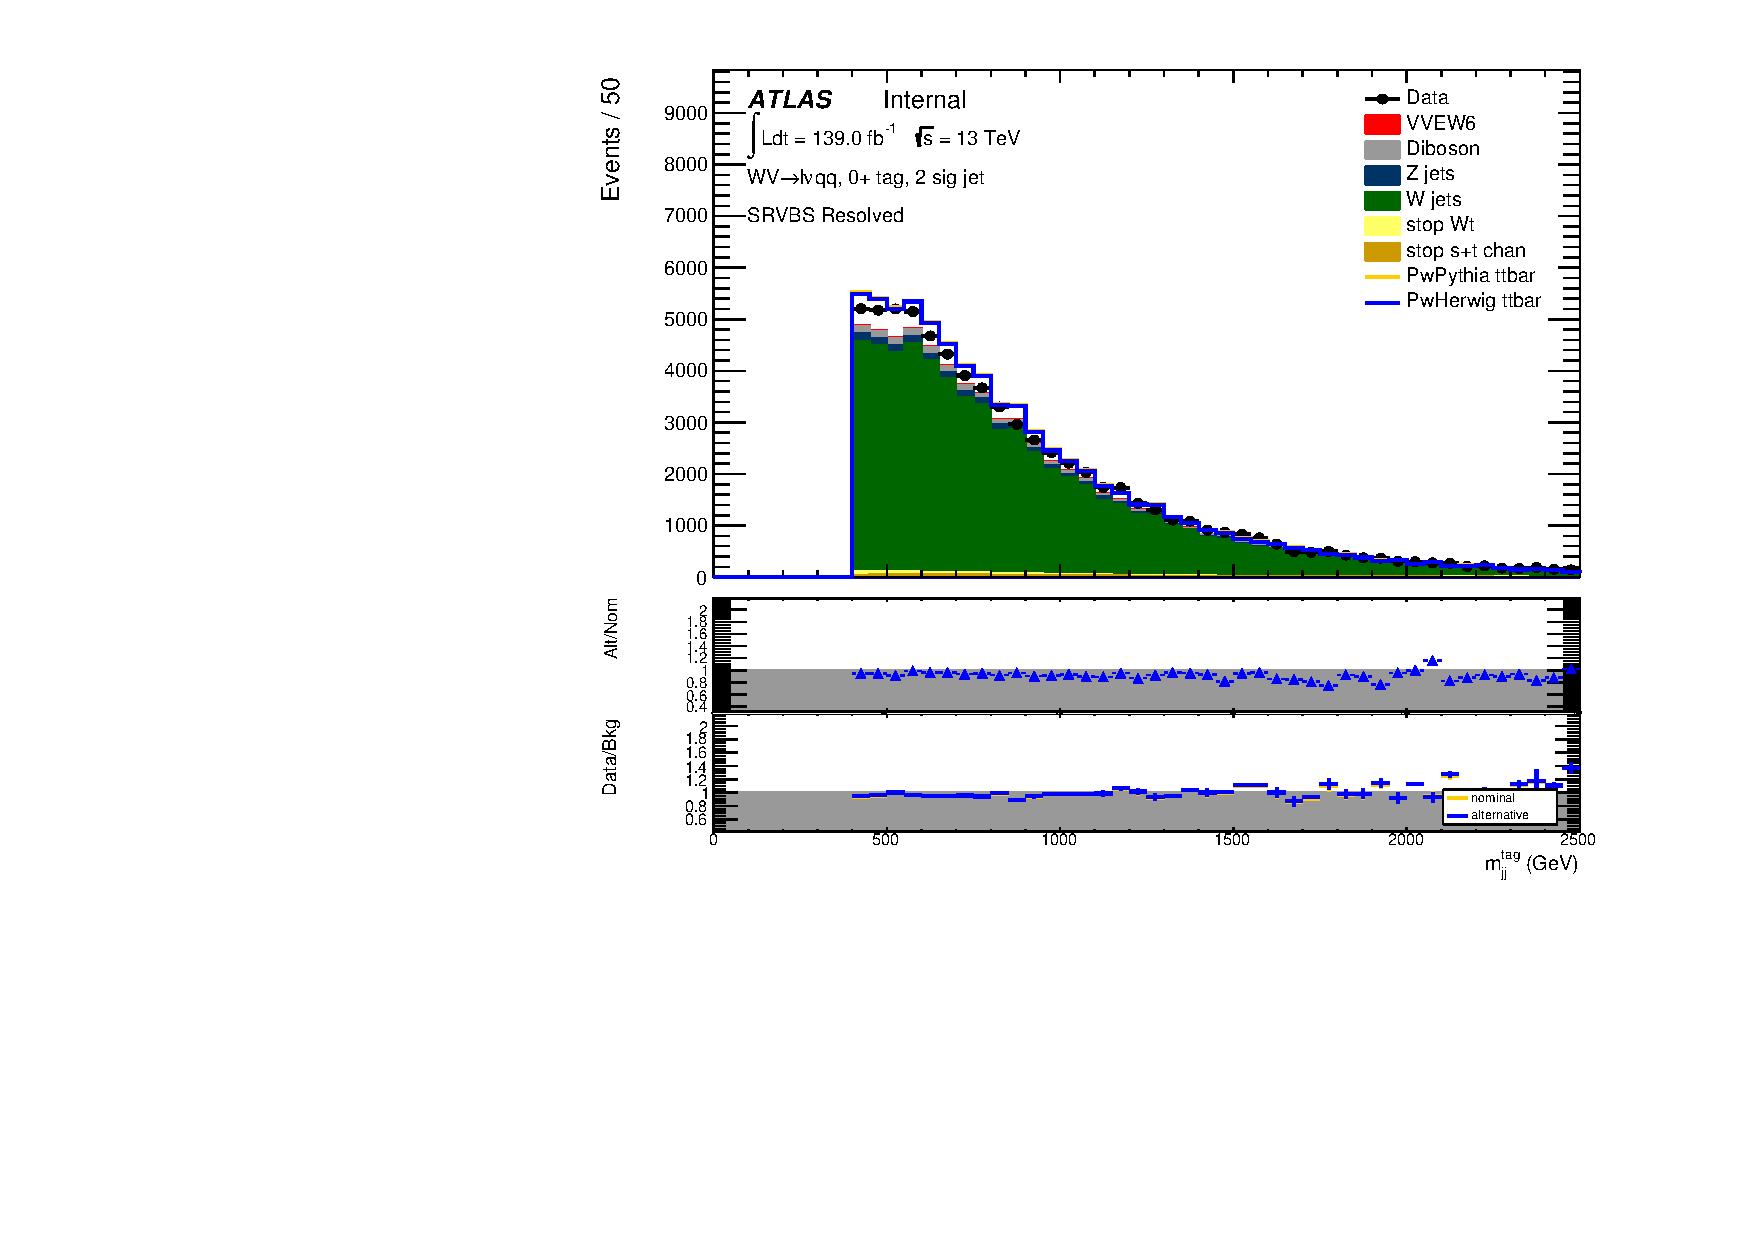
\includegraphics[width=0.3\textwidth]{figures/1lep/ModelUnc/ttbarPwHg/C_0ptag2pjet_0ptv_SRVBS_Tight_tagMjj_Lin.pdf}}
        \subfigure[ttbar shower uncertainties for mjjtag in the merged HP signal region]{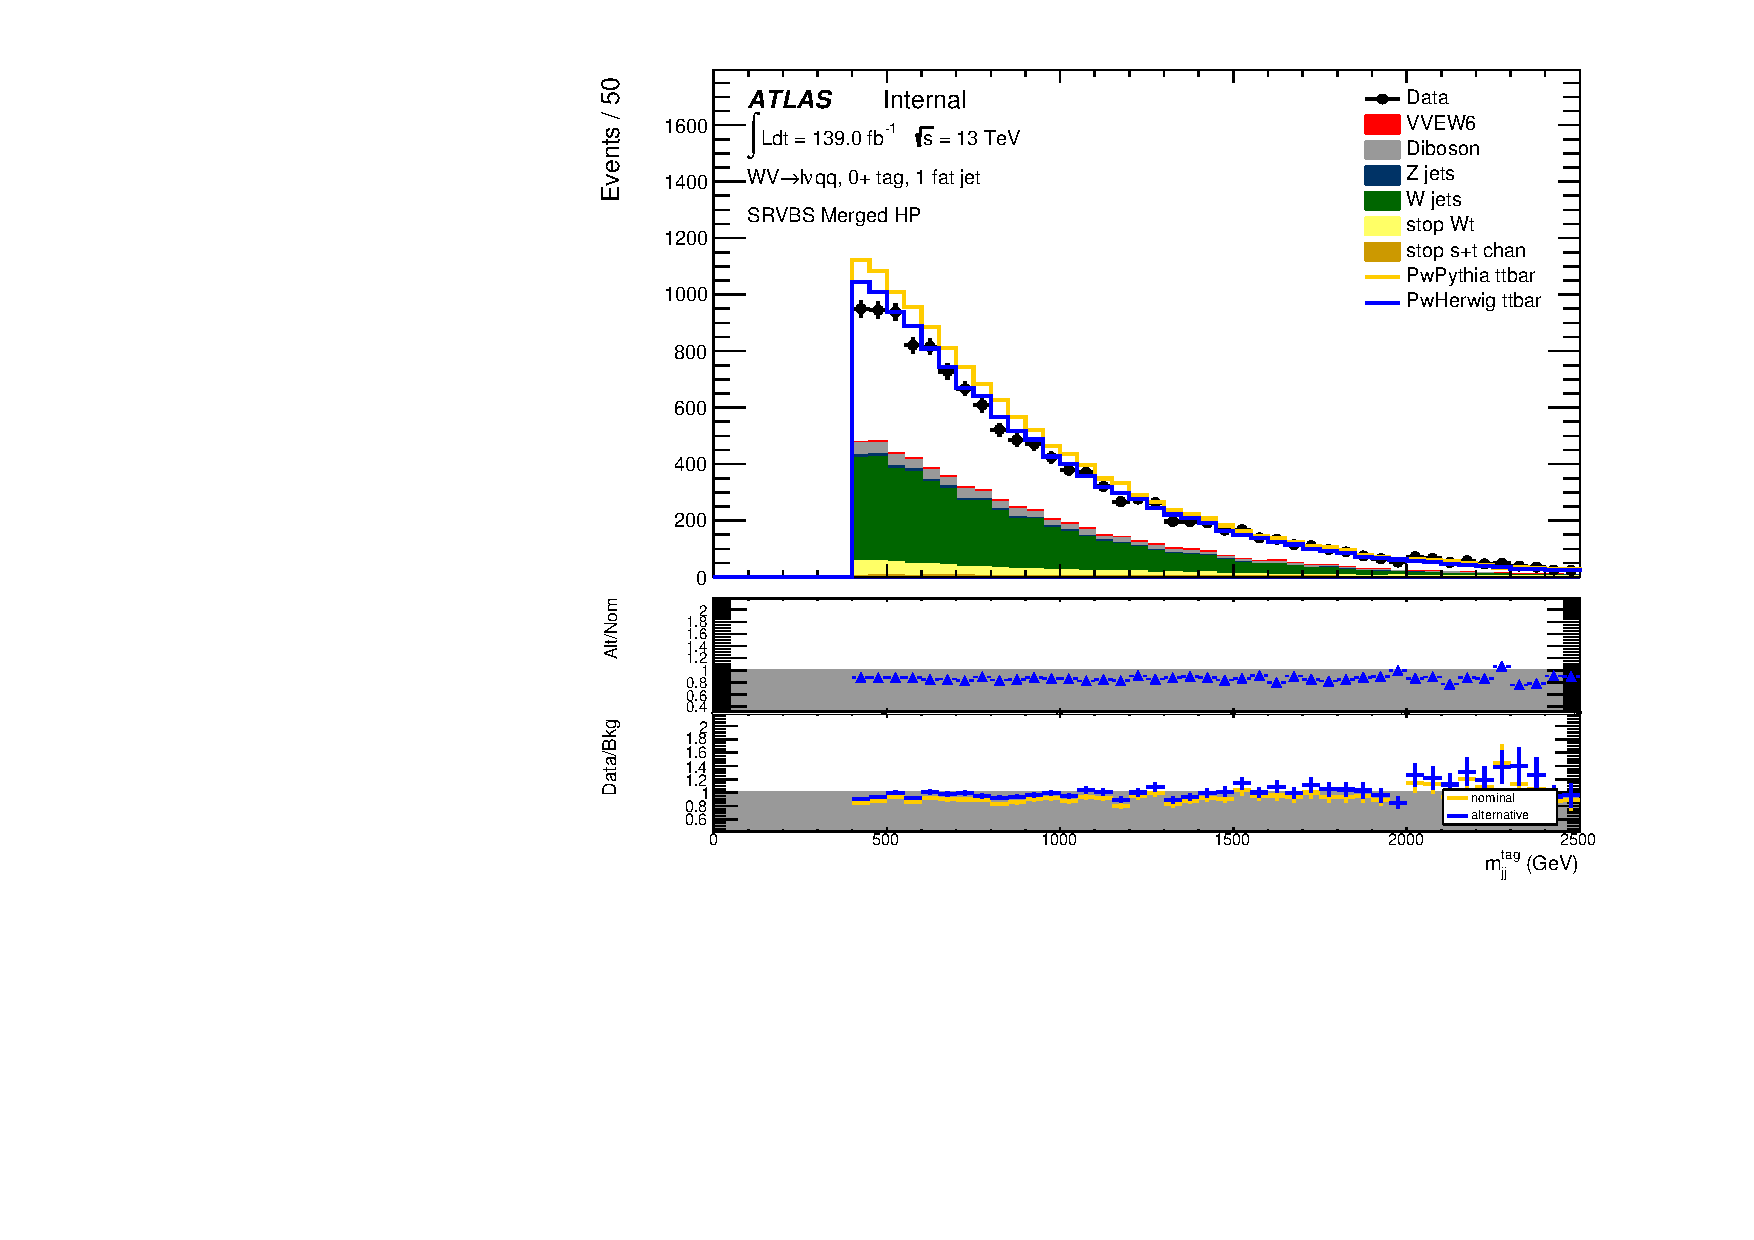
\includegraphics[width=0.3\textwidth]{figures/1lep/ModelUnc/ttbarPwHg/C_0ptag1pfat0pjet_0ptv_SRVBS_HP_tagMjj_Lin.pdf}}
        \subfigure[ttbar shower uncertainties for mjjtag in the merged LP signal region]{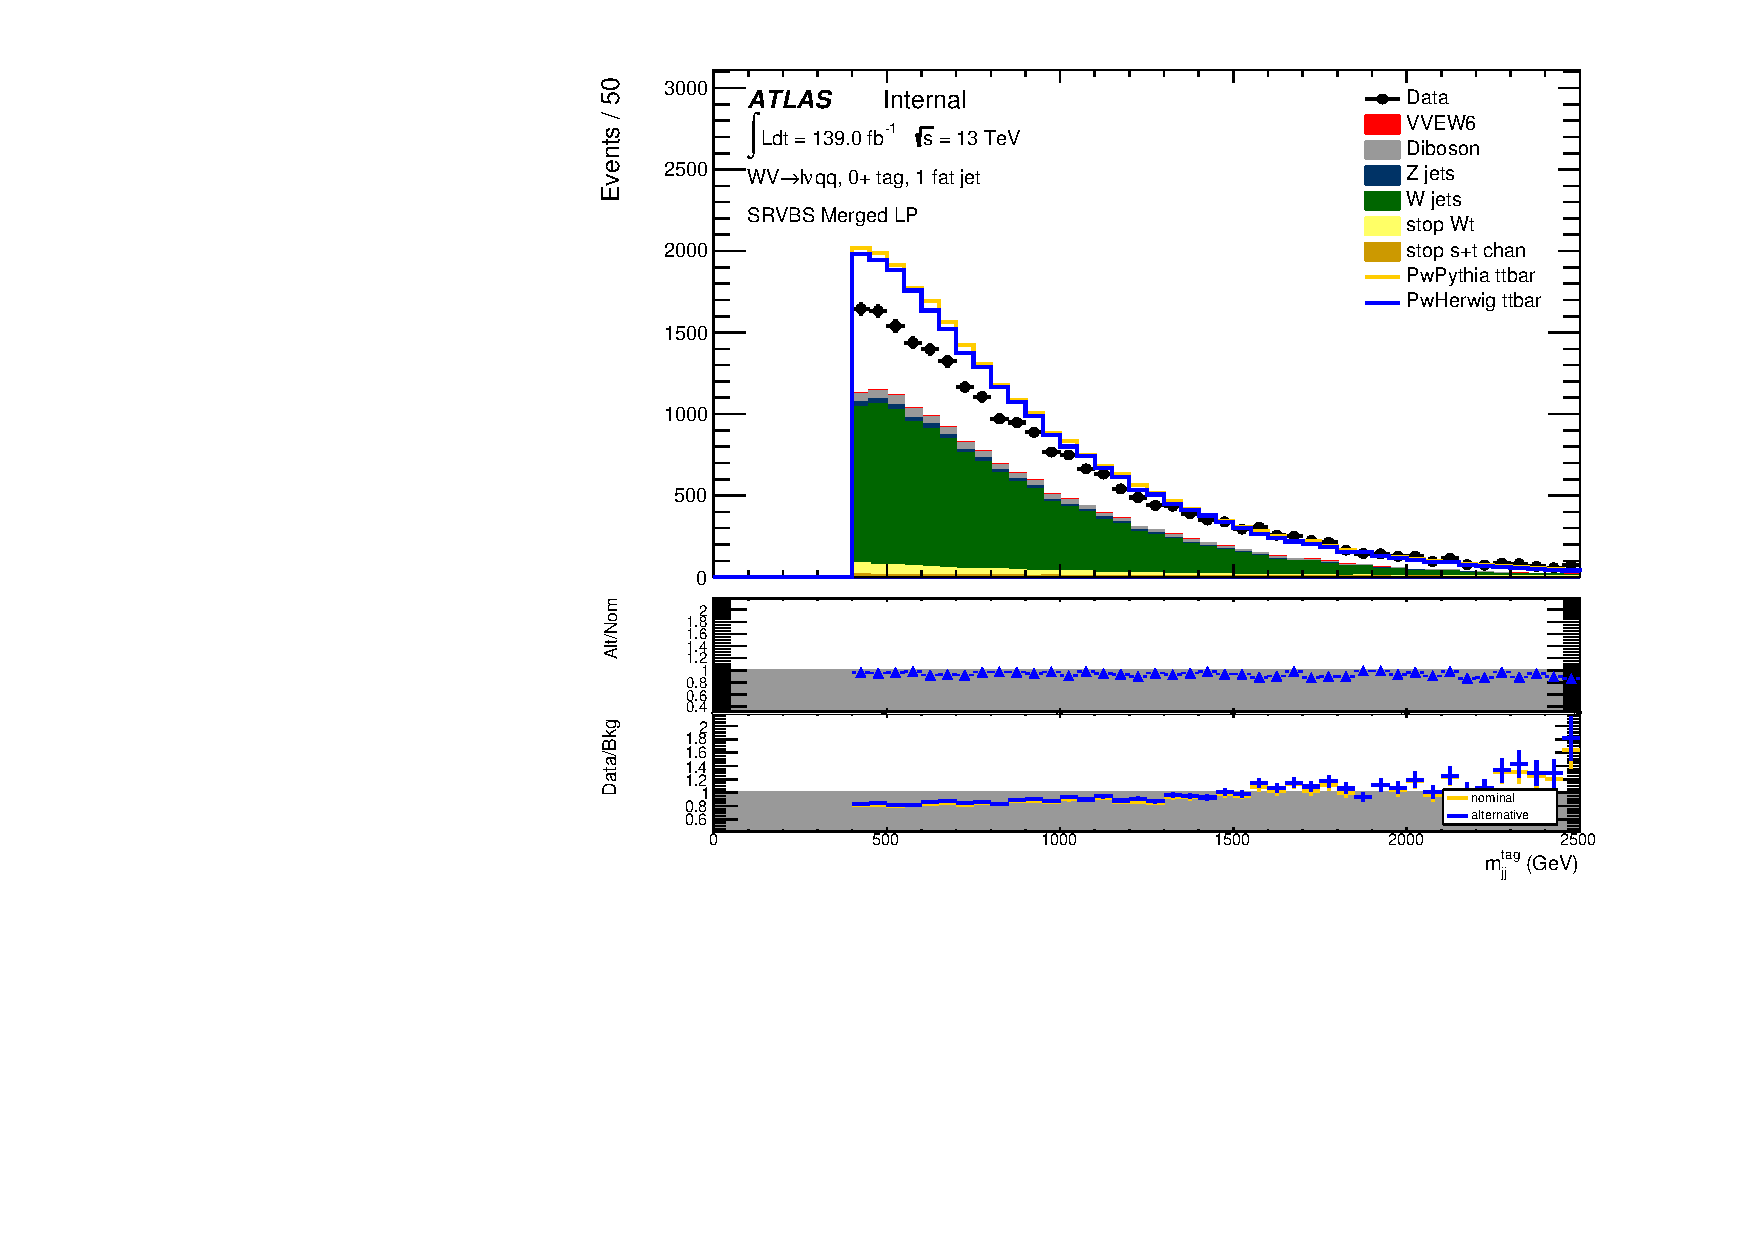
\includegraphics[width=0.3\textwidth]{figures/1lep/ModelUnc/ttbarPwHg/C_0ptag1pfat0pjet_0ptv_SRVBS_LP_tagMjj_Lin.pdf}}\\
        \subfigure[ttbar shower uncertainties for RNN score in the resolved signal region]{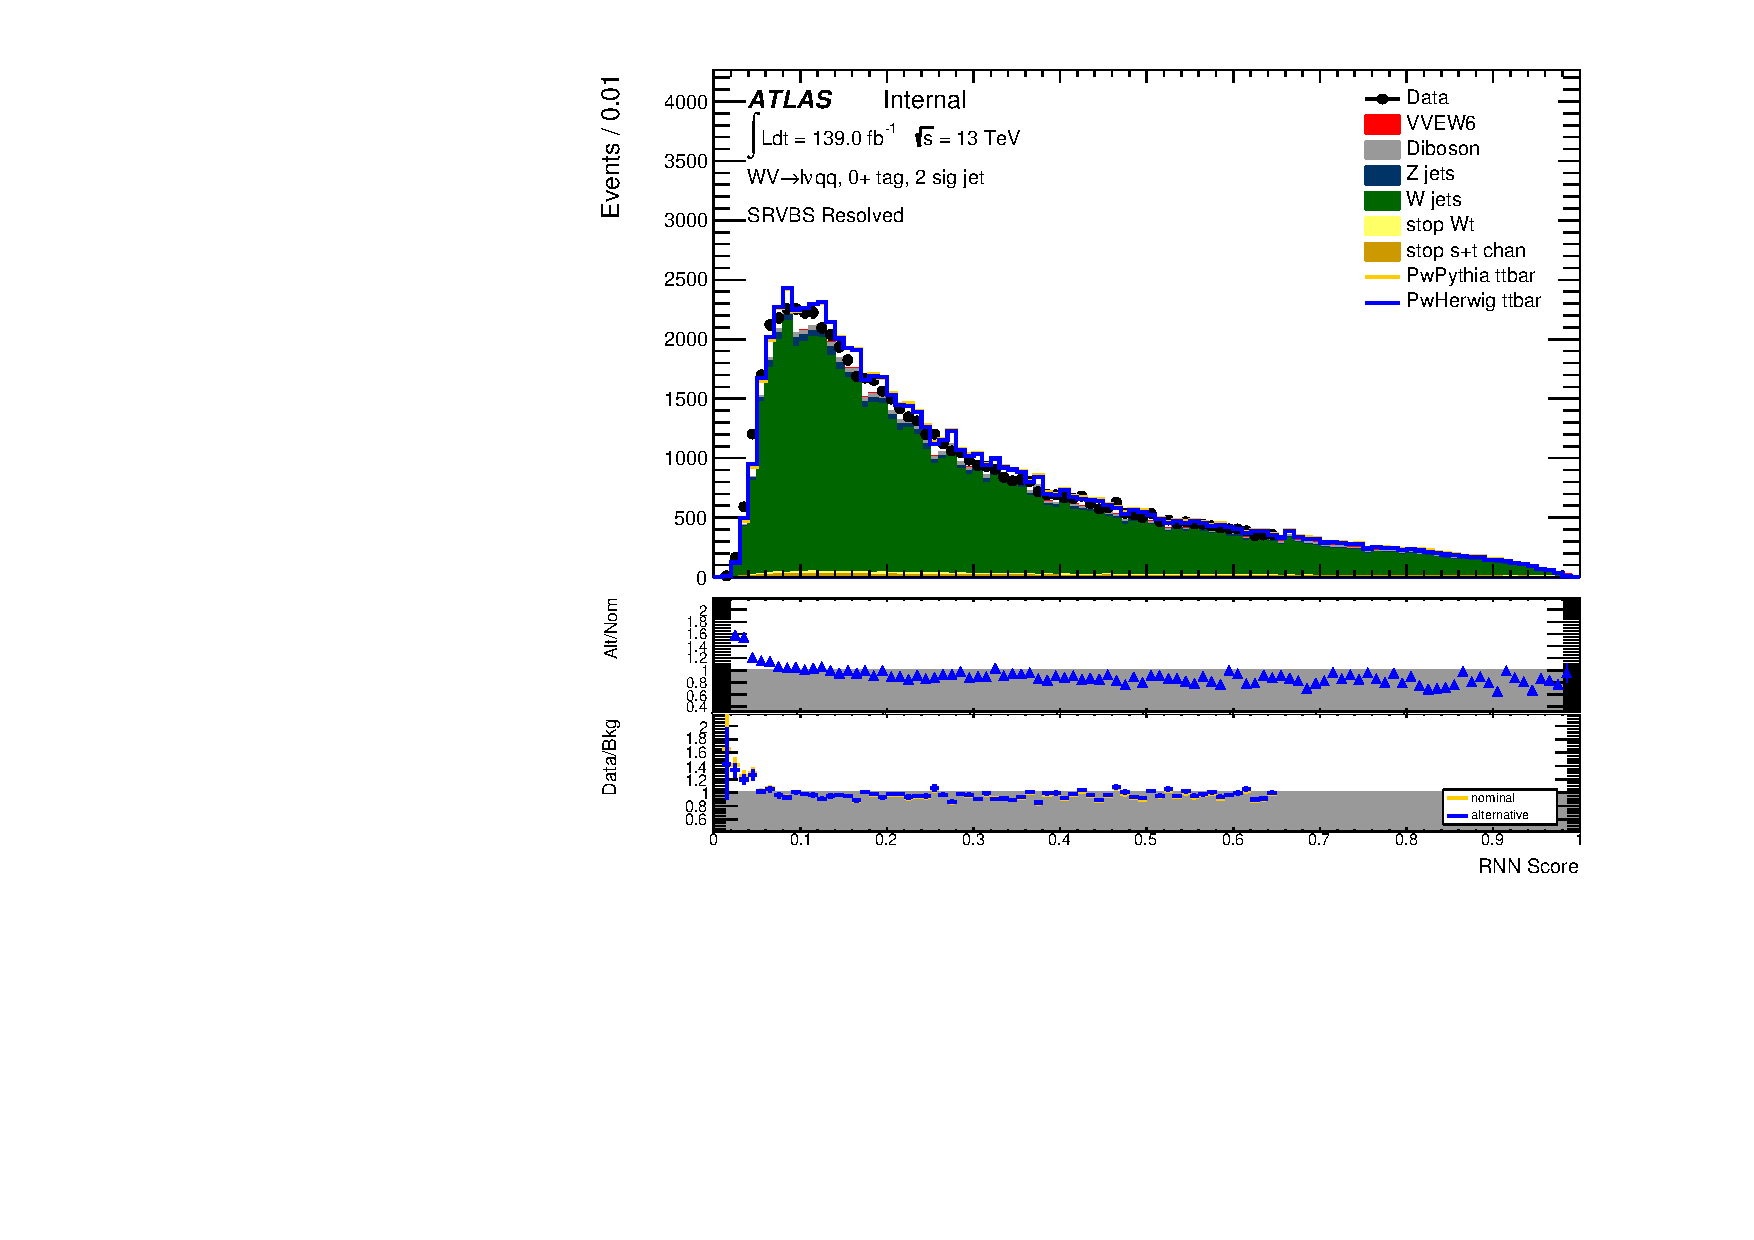
\includegraphics[width=0.3\textwidth]{figures/1lep/ModelUnc/ttbarPwHg/C_0ptag2pjet_0ptv_SRVBS_Tight_RNN_Lin.pdf}}
        \subfigure[ttbar shower uncertainties for RNN score in the merged HP signal region]{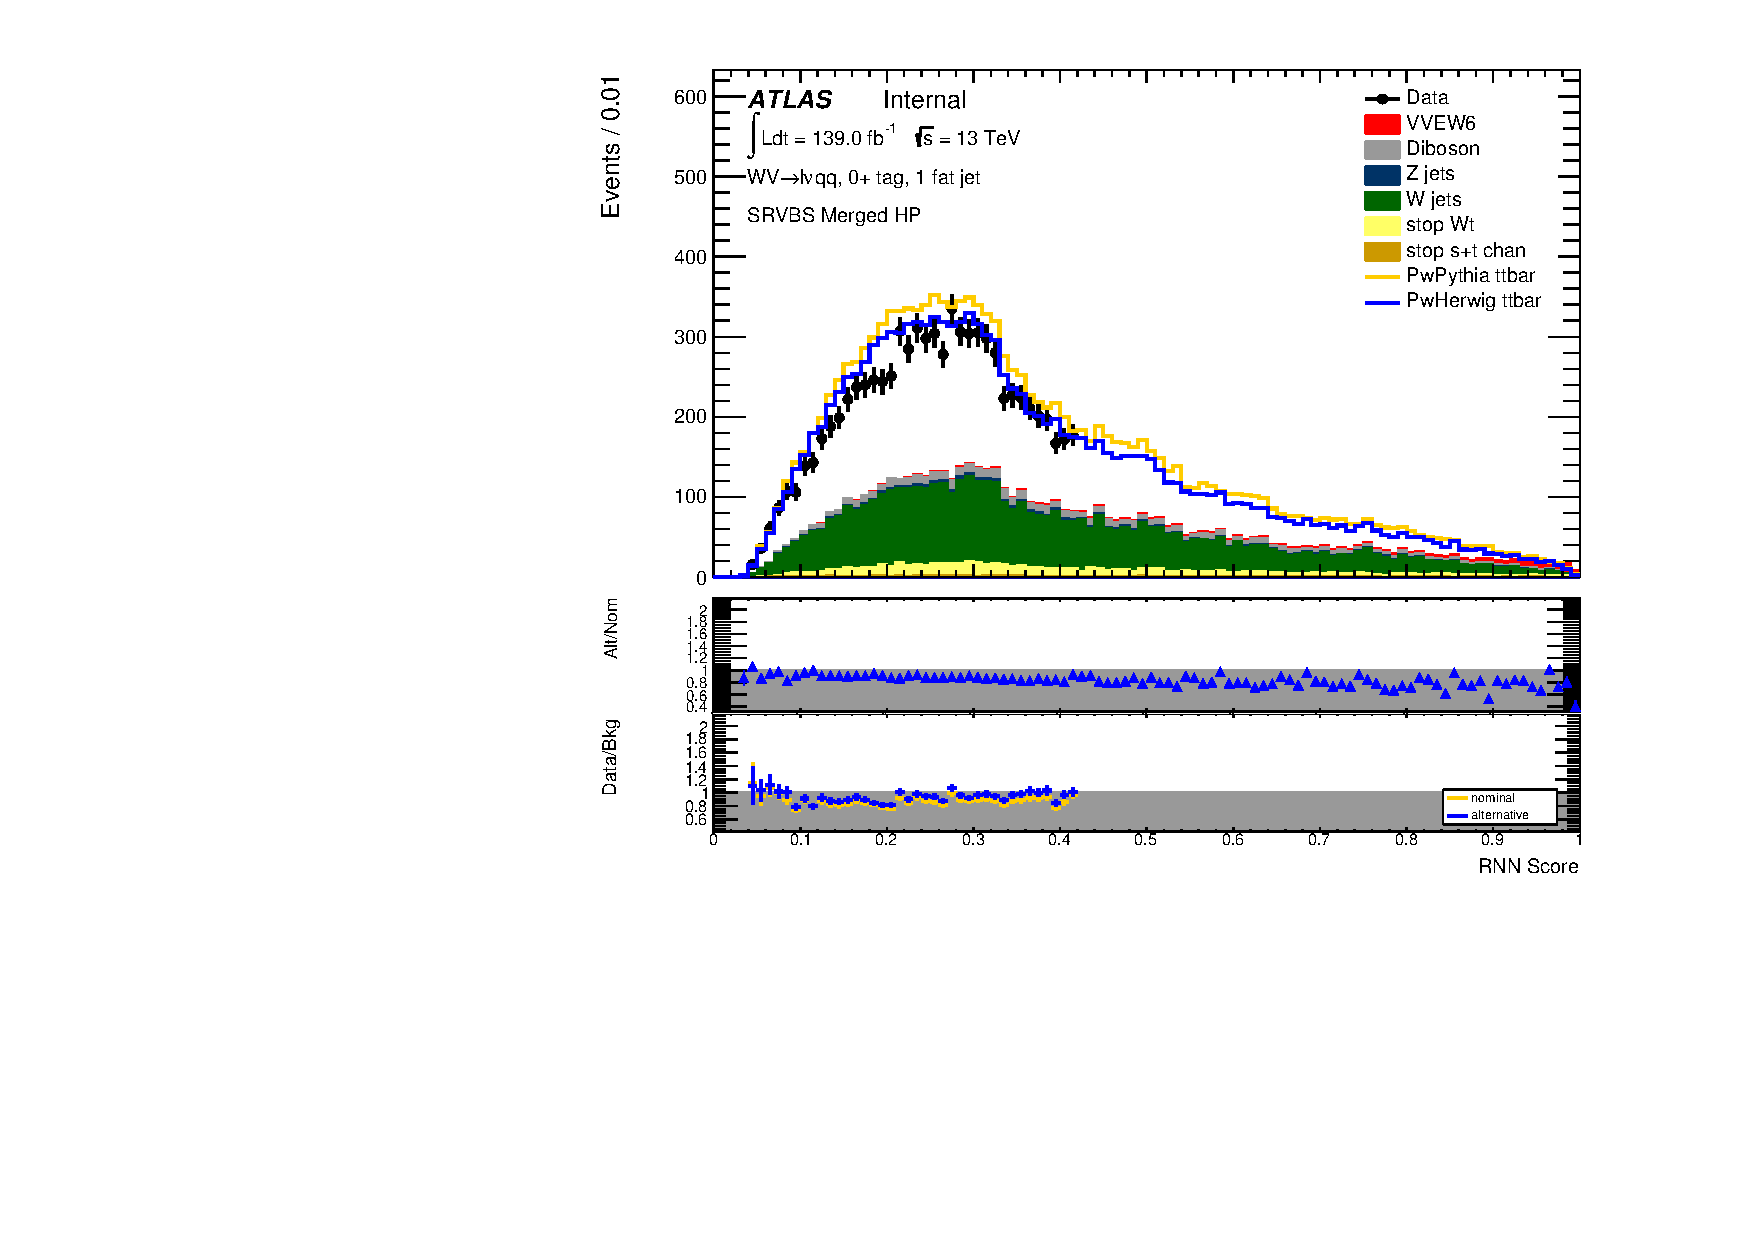
\includegraphics[width=0.3\textwidth]{figures/1lep/ModelUnc/ttbarPwHg/C_0ptag1pfat0pjet_0ptv_SRVBS_HP_RNN_Lin.pdf}}
        \subfigure[ttbar shower uncertainties for RNN score in the merged LP signal region]{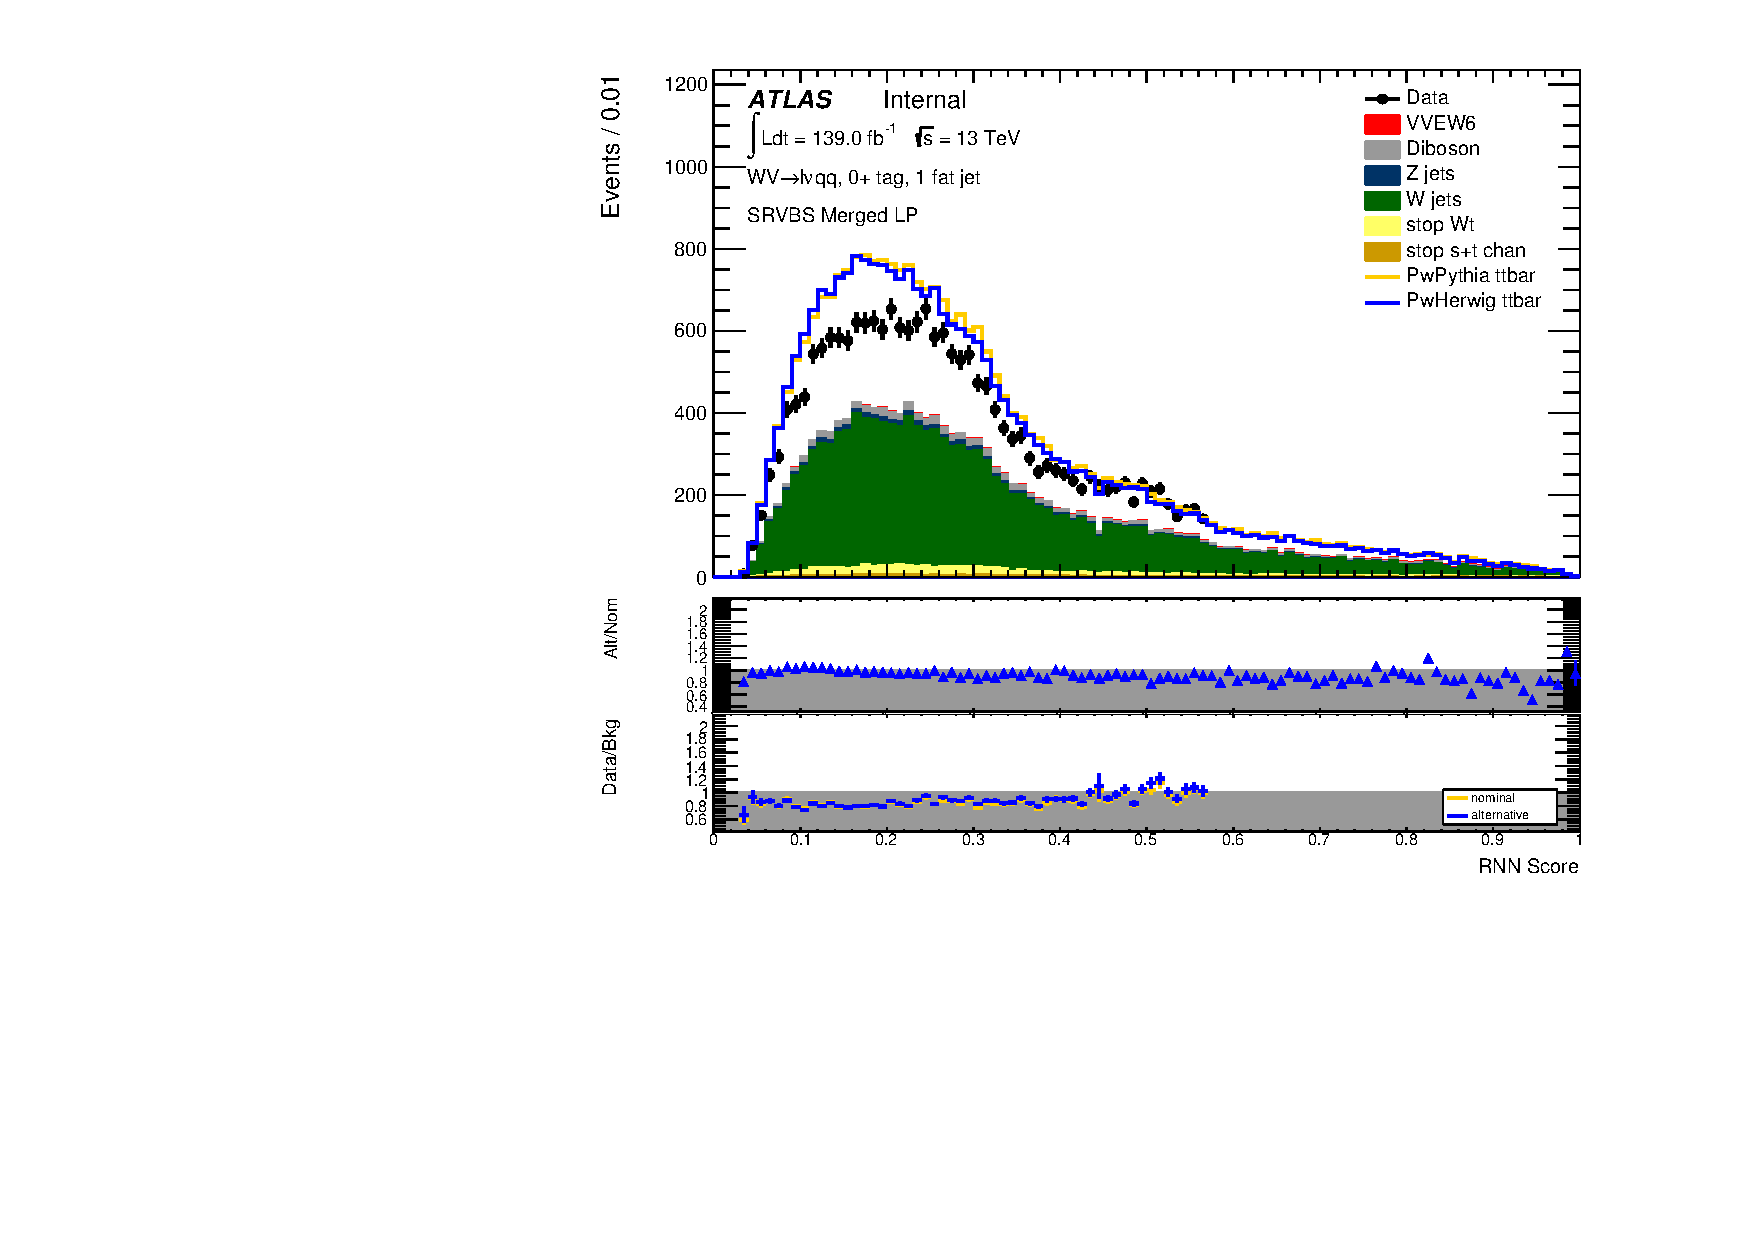
\includegraphics[width=0.3\textwidth]{figures/1lep/ModelUnc/ttbarPwHg/C_0ptag1pfat0pjet_0ptv_SRVBS_LP_RNN_Lin.pdf}}
        \caption{Modelling uncertainties derived from PowhegPythia nominal ttbar samples and PowhegHerwig alternative ttbar samples.}
    \label{fig:ModelUncttbar1Lep}
\end{figure}
	
\begin{figure}[ht]
    \centering
	\subfigure[ttbar hard scatter uncertainties for mjjtag in the resolved top control region]{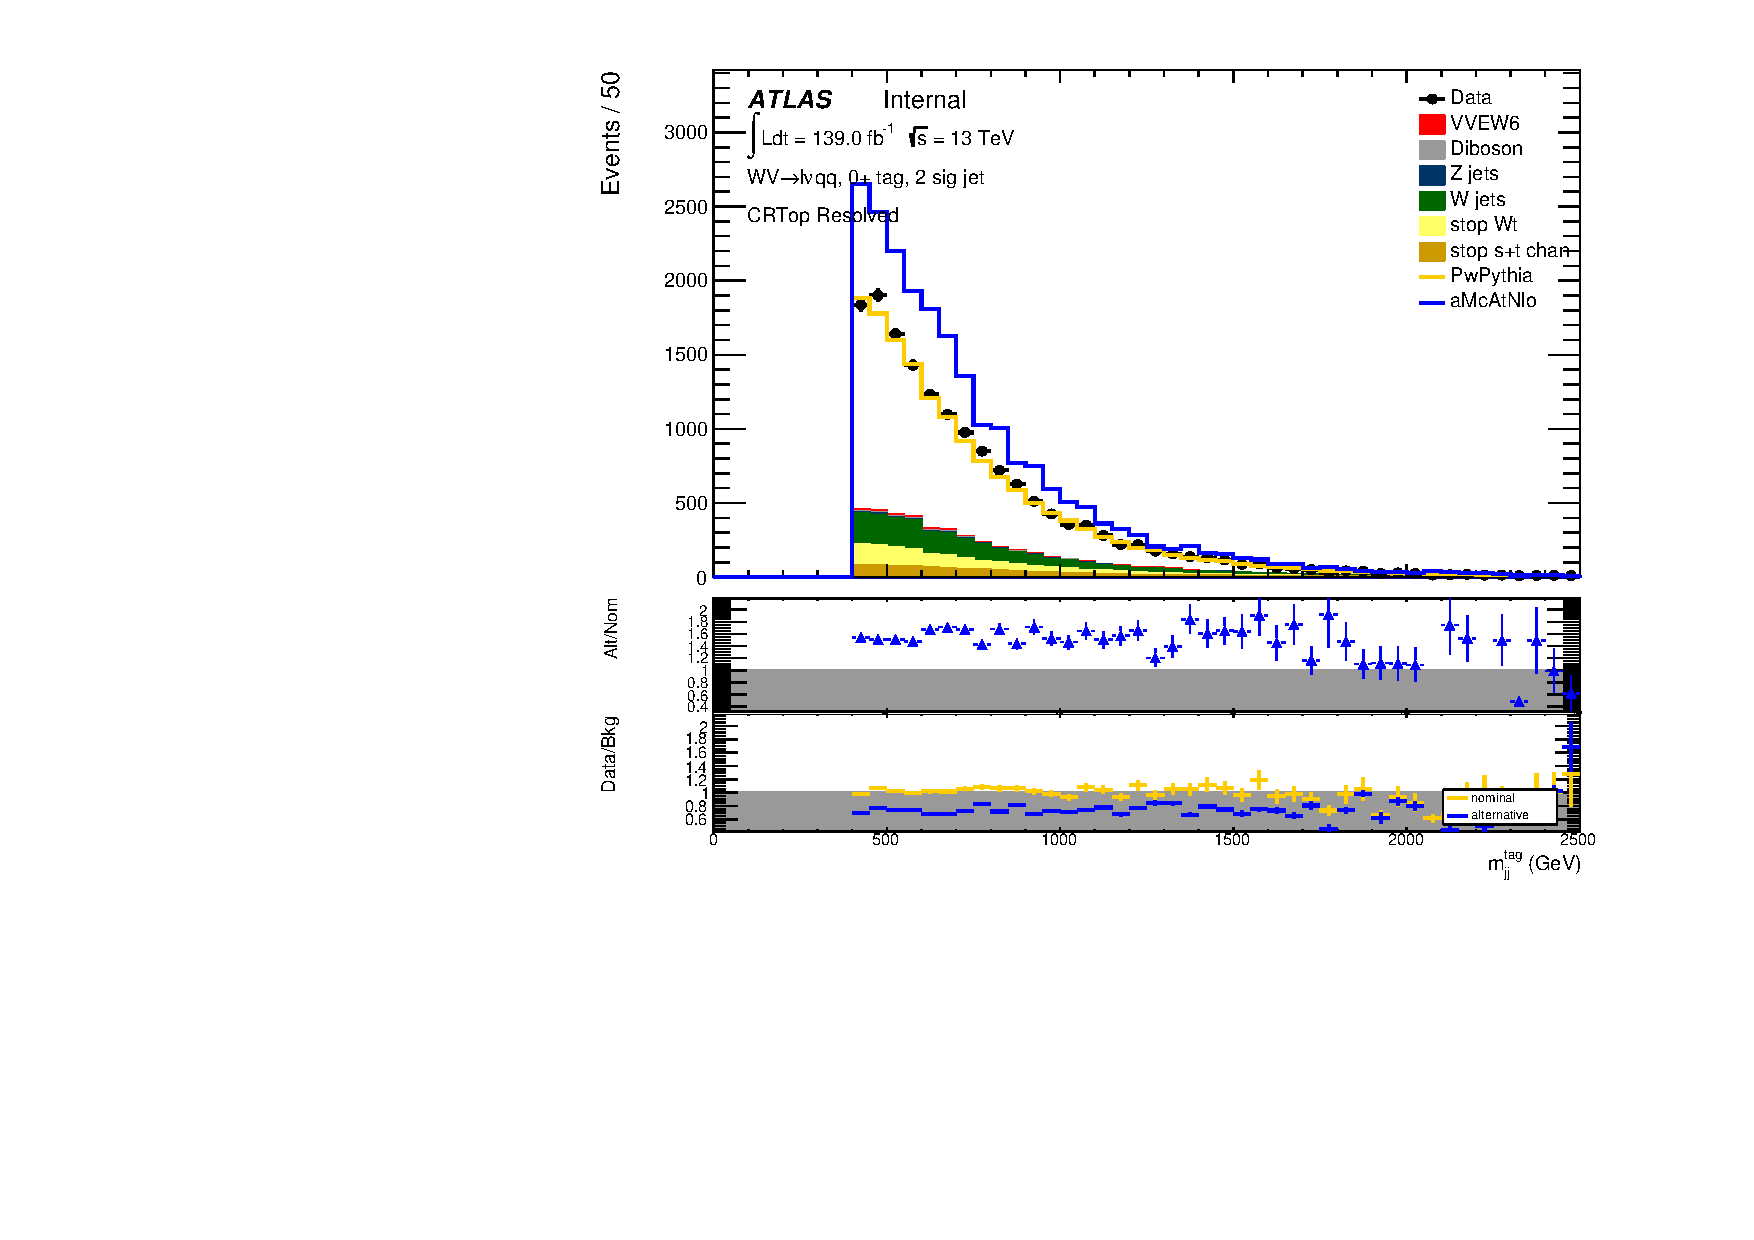
\includegraphics[width=0.3\textwidth]{figures/1lep/ModelUnc/ttbarnoShWe/C_0ptag2pjet_0ptv_CRTop_Tight_tagMjj_Lin.pdf}}
        \subfigure[ttbar hard scatter uncertainties for mjjtag in the merged HP top control region]{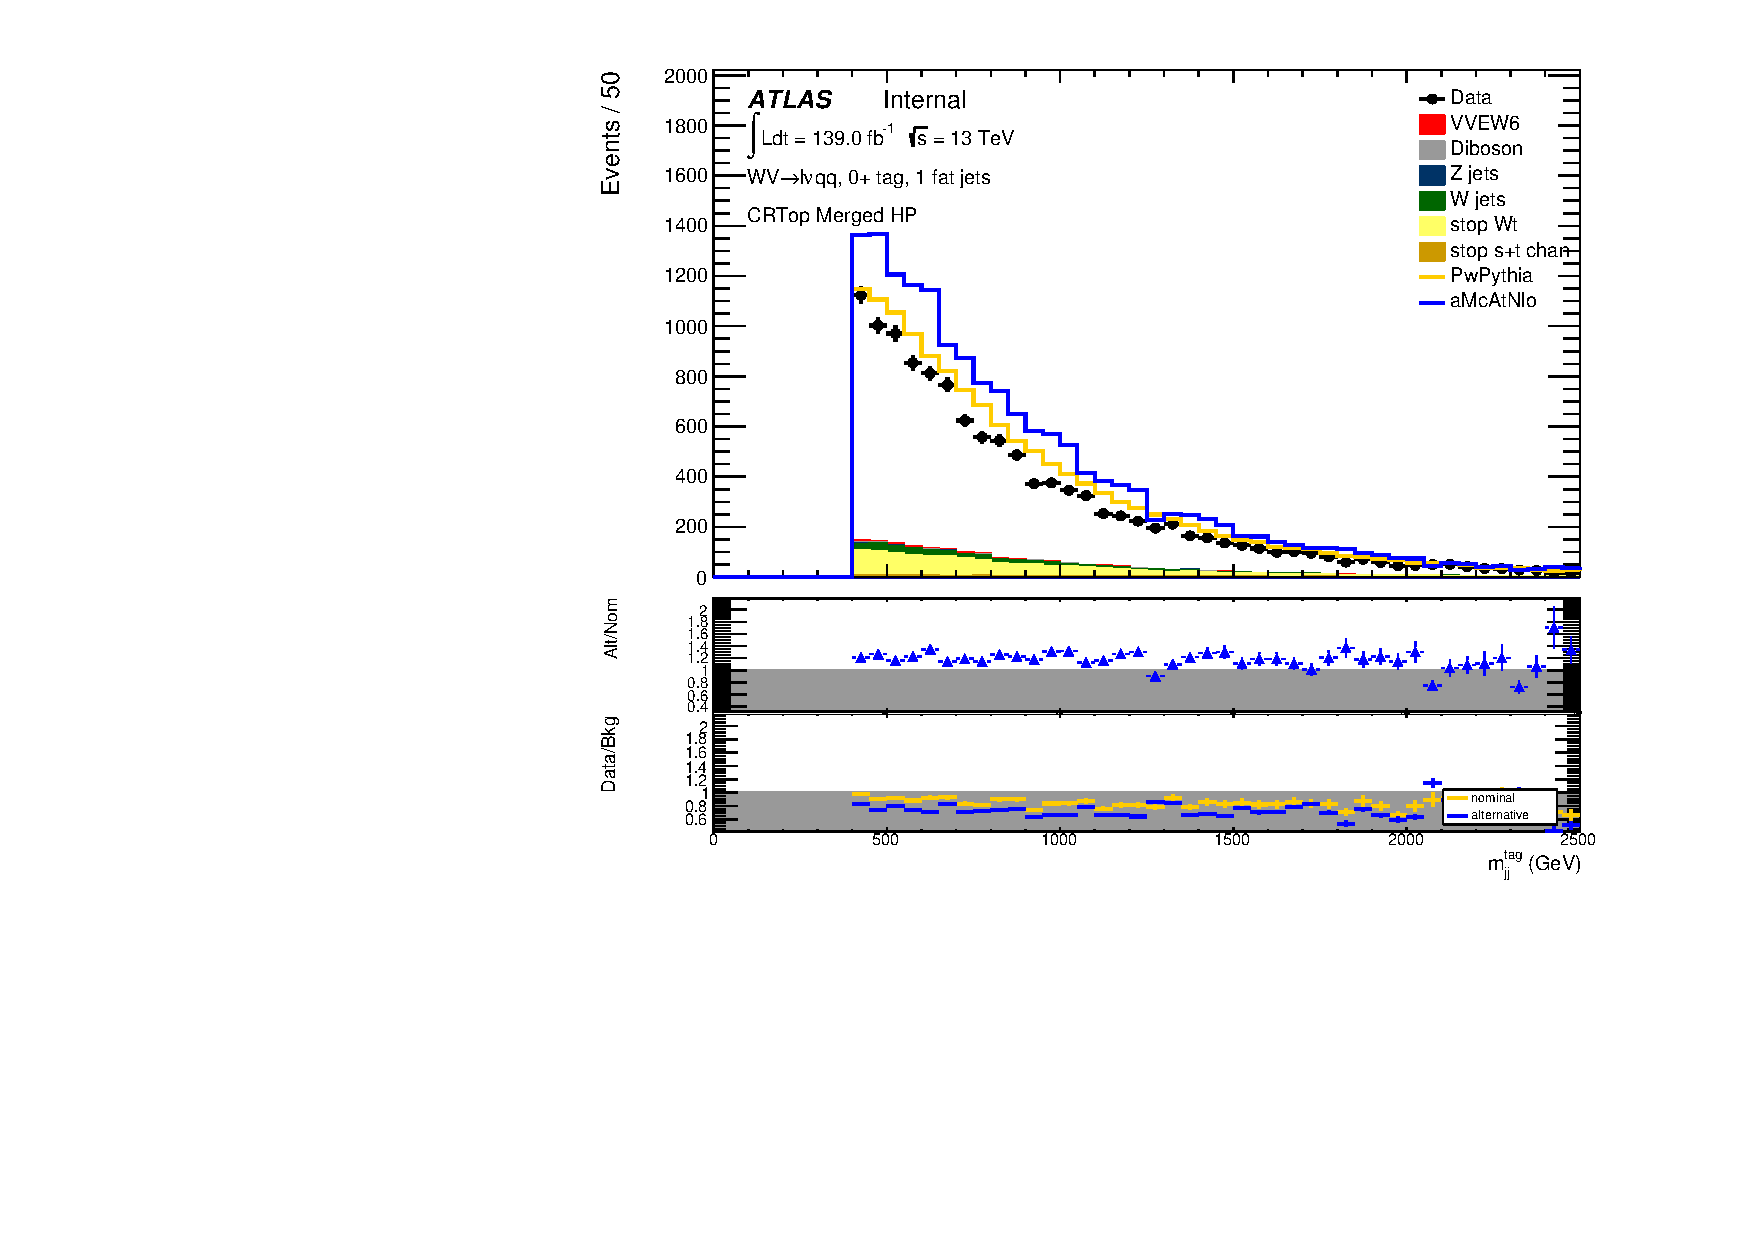
\includegraphics[width=0.3\textwidth]{figures/1lep/ModelUnc/ttbarnoShWe/C_0ptag1pfat0pjet_0ptv_CRTop_HP_tagMjj_Lin.pdf}}
        \subfigure[ttbar hard scatter uncertainties for mjjtag in the merged LP top control region]{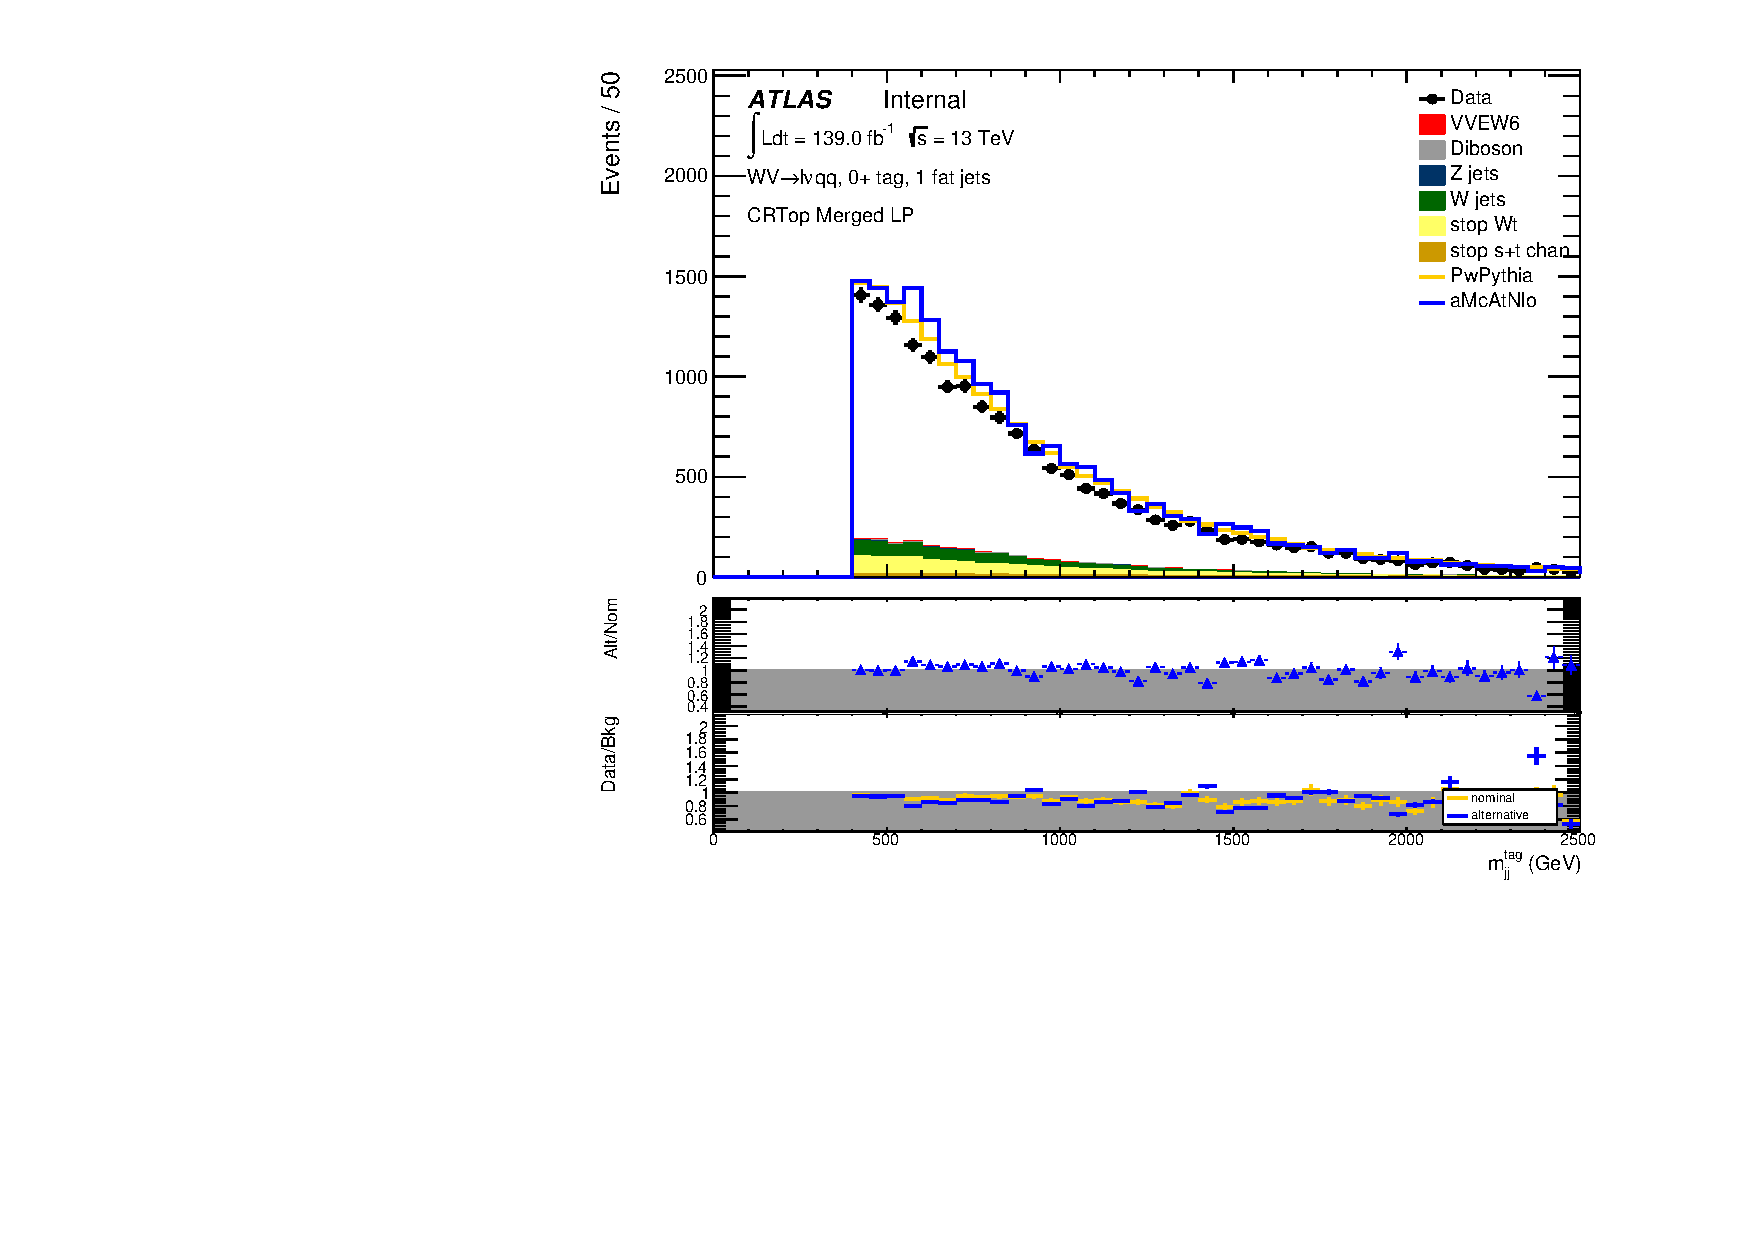
\includegraphics[width=0.3\textwidth]{figures/1lep/ModelUnc/ttbarnoShWe/C_0ptag1pfat0pjet_0ptv_CRTop_LP_tagMjj_Lin.pdf}}\\
        \subfigure[ttbar hard scatter uncertainties for RNN score in the resolved top control region]{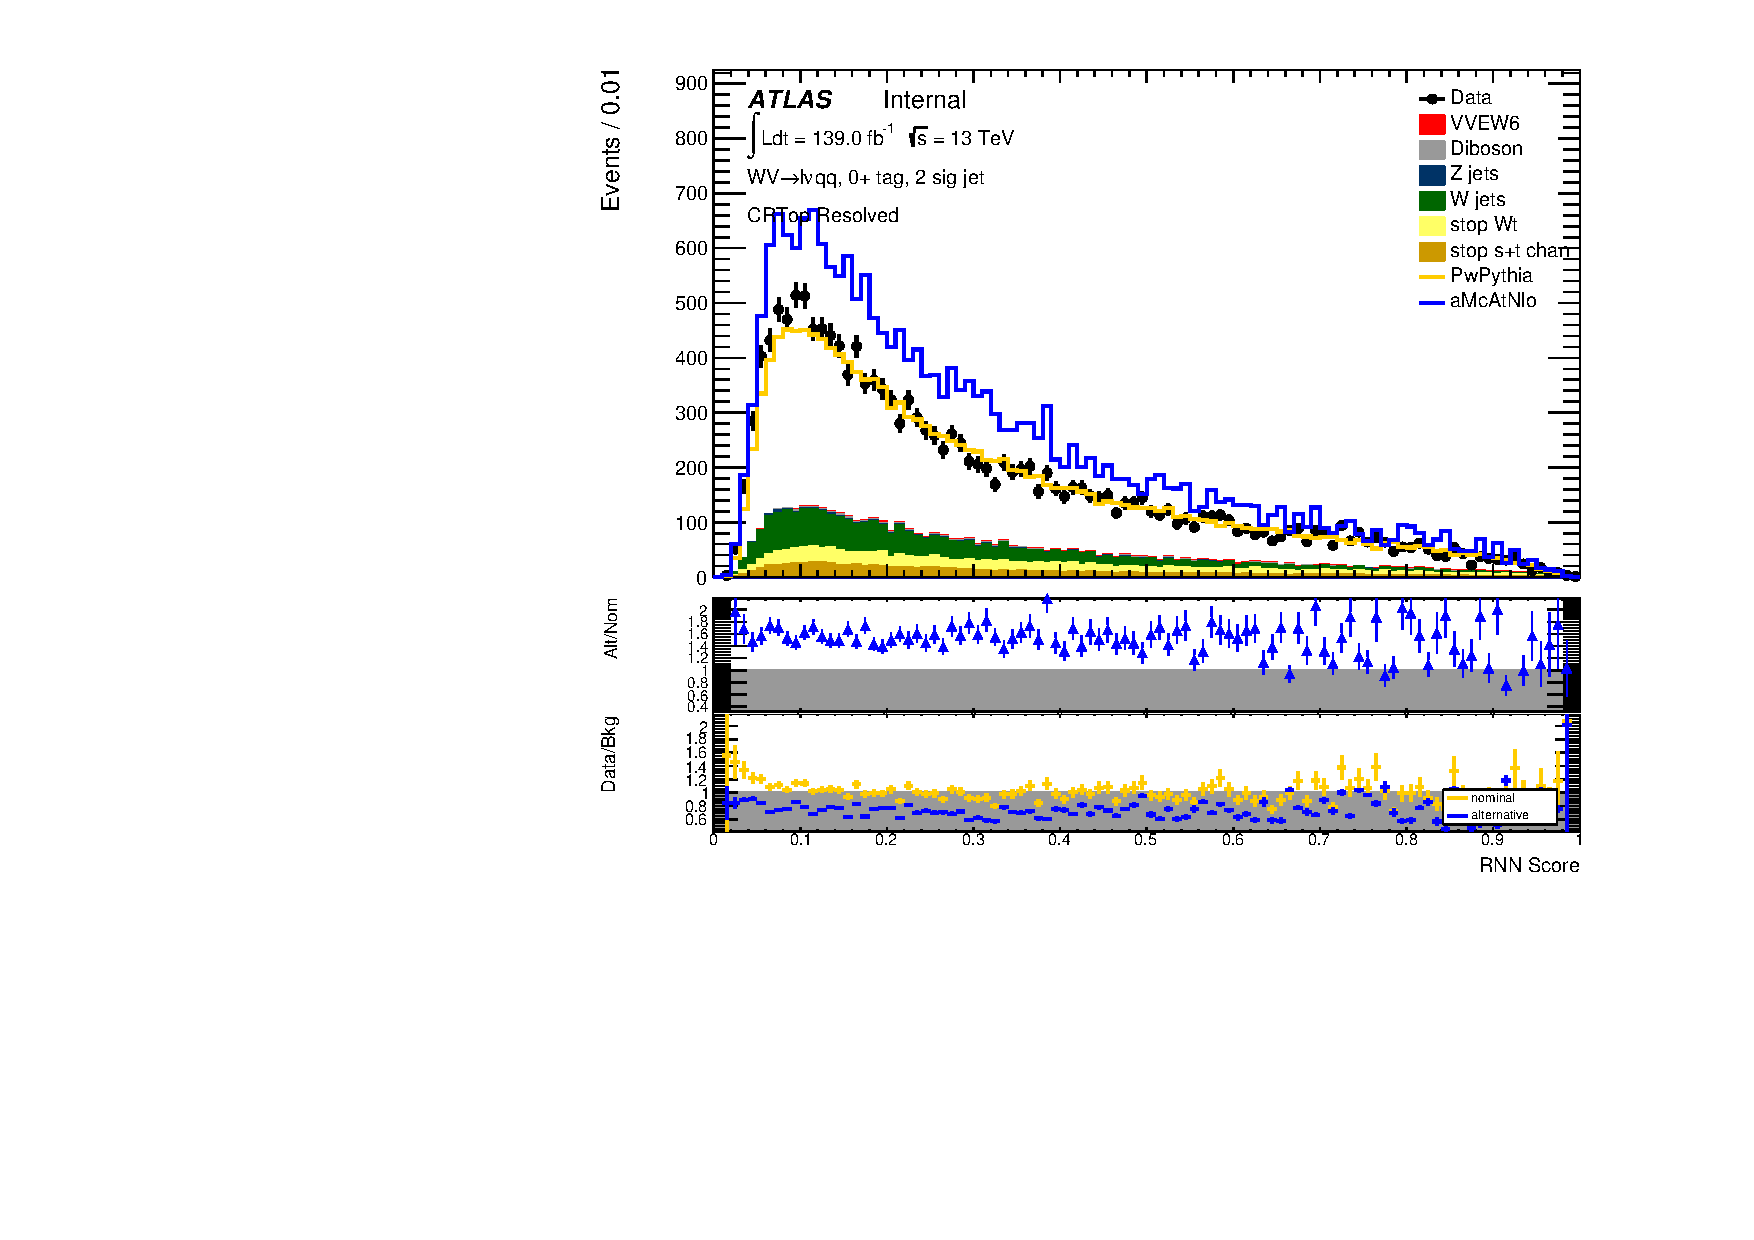
\includegraphics[width=0.3\textwidth]{figures/1lep/ModelUnc/ttbarnoShWe/C_0ptag2pjet_0ptv_CRTop_Tight_RNN_Lin.pdf}}
        \subfigure[ttbar hard scatter uncertainties for RNN score in the merged HP top control region]{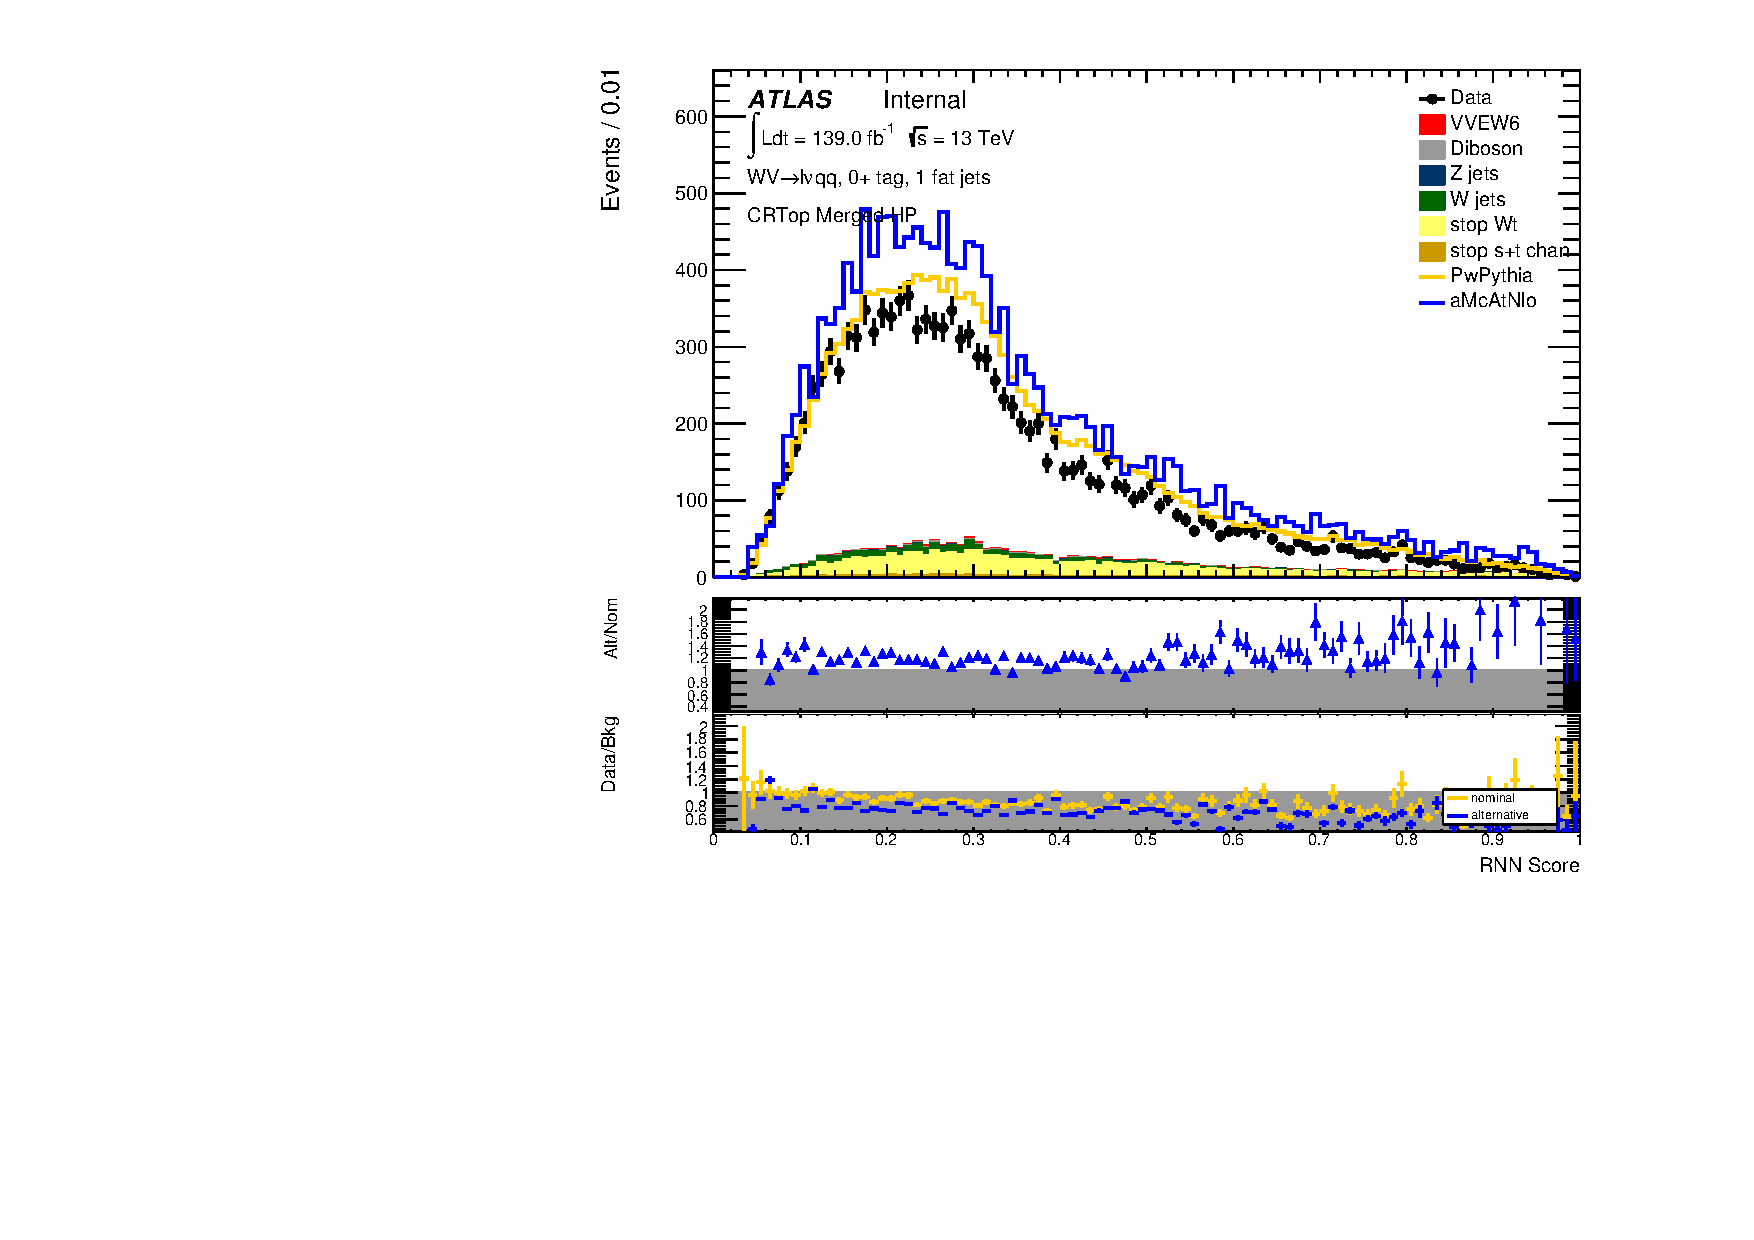
\includegraphics[width=0.3\textwidth]{figures/1lep/ModelUnc/ttbarnoShWe/C_0ptag1pfat0pjet_0ptv_CRTop_HP_RNN_Lin.pdf}}
        \subfigure[ttbar hard scatter uncertainties for RNN score in the merged LP top control region]{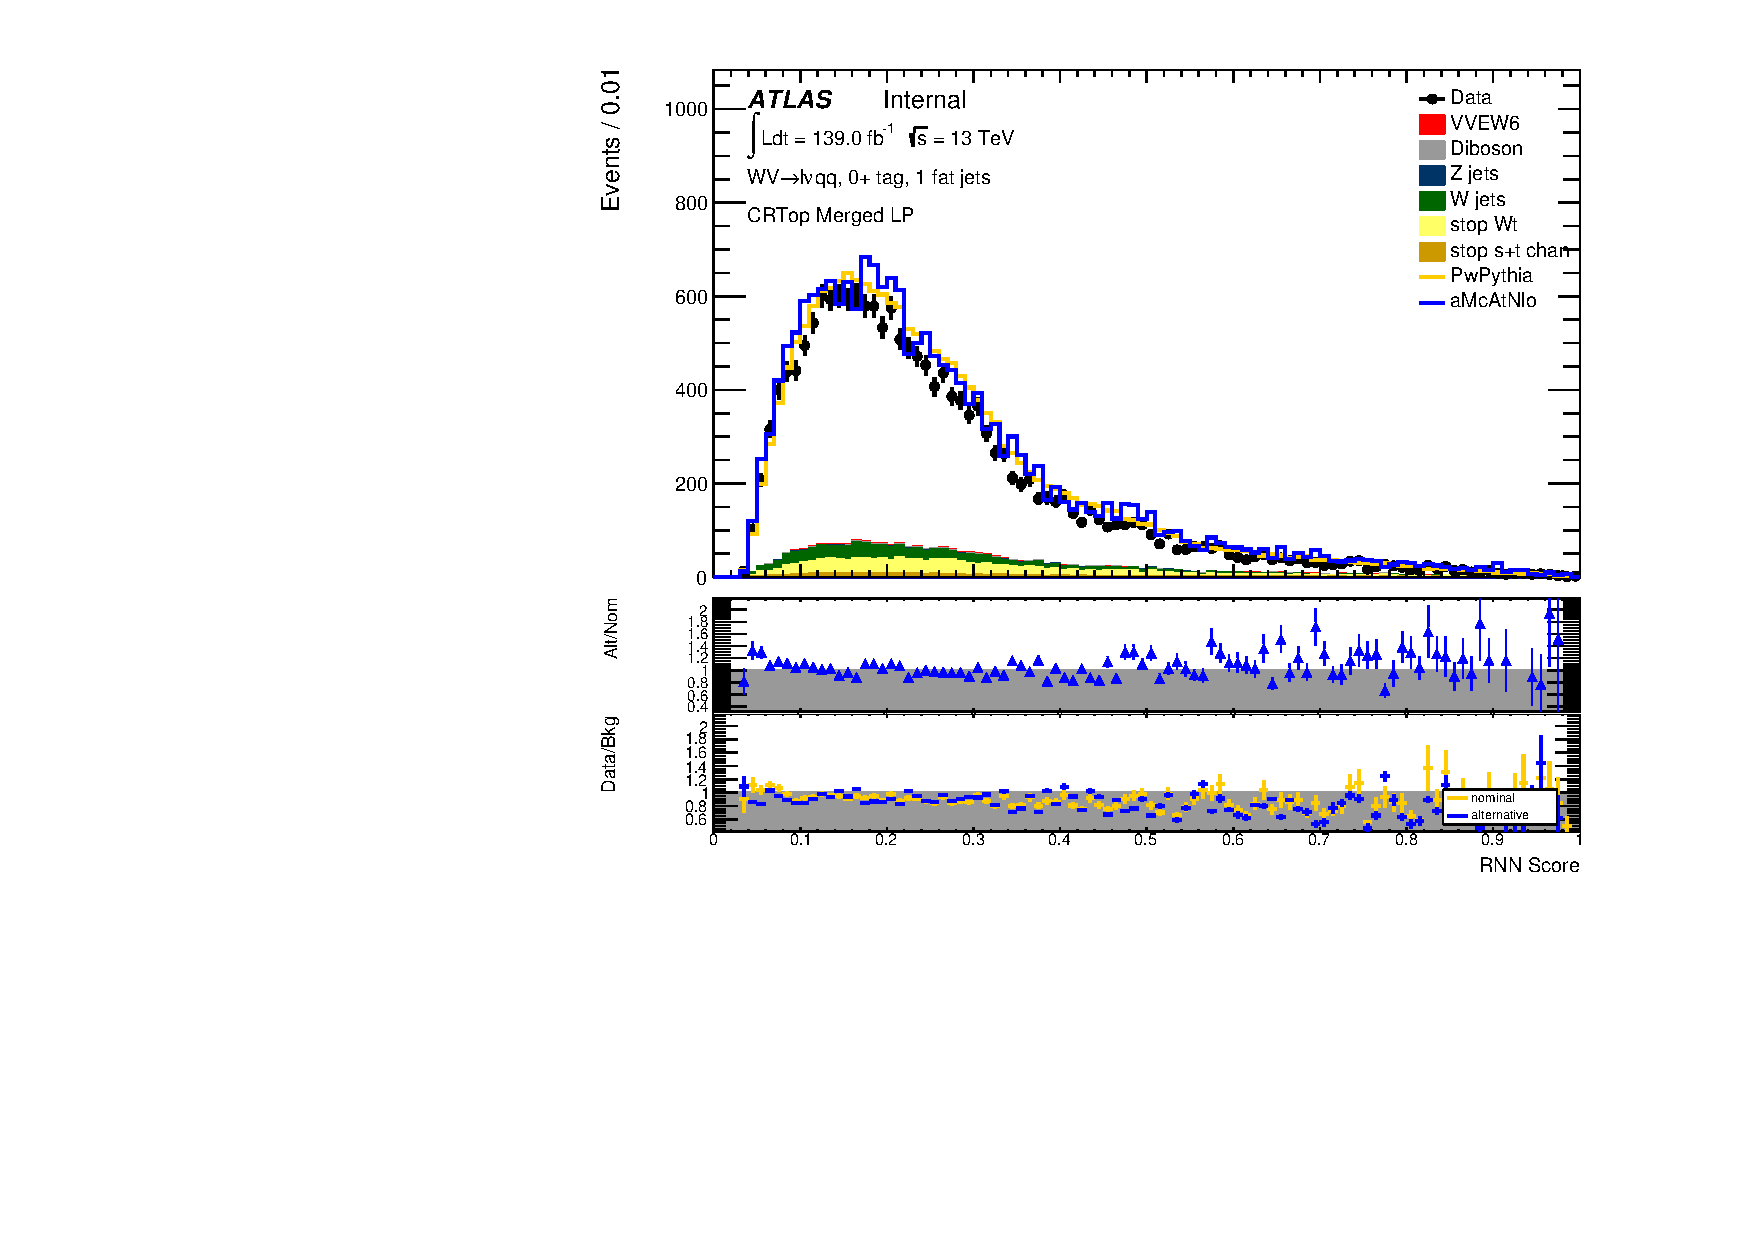
\includegraphics[width=0.3\textwidth]{figures/1lep/ModelUnc/ttbarnoShWe/C_0ptag1pfat0pjet_0ptv_CRTop_LP_RNN_Lin.pdf}}\\
        \subfigure[ttbar hard scatter uncertainties for mjjtag in the resolved signal region]{\includegraphics[width=0.3\textwidth]{figures/1lep/ModelUnc/ttbarnoShWe/C_0ptag2pjet_0ptv_SRVBS_Tight_tagMjj_Lin.pdf}}
        \subfigure[ttbar hard scatter uncertainties for mjjtag in the merged HP signal region]{\includegraphics[width=0.3\textwidth]{figures/1lep/ModelUnc/ttbarnoShWe/C_0ptag1pfat0pjet_0ptv_SRVBS_HP_tagMjj_Lin.pdf}}
        \subfigure[ttbar hard scatter uncertainties for mjjtag in the merged LP signal region]{\includegraphics[width=0.3\textwidth]{figures/1lep/ModelUnc/ttbarnoShWe/C_0ptag1pfat0pjet_0ptv_SRVBS_LP_tagMjj_Lin.pdf}}\\
        \subfigure[ttbar hard scatter uncertainties for RNN score in the resolved signal region]{\includegraphics[width=0.3\textwidth]{figures/1lep/ModelUnc/ttbarnoShWe/C_0ptag2pjet_0ptv_SRVBS_Tight_RNN_Lin.pdf}}
        \subfigure[ttbar hard scatter uncertainties for RNN score in the merged HP signal region]{\includegraphics[width=0.3\textwidth]{figures/1lep/ModelUnc/ttbarnoShWe/C_0ptag1pfat0pjet_0ptv_SRVBS_HP_RNN_Lin.pdf}}
        \subfigure[ttbar hard scatter uncertainties for RNN score in the merged LP signal region]{\includegraphics[width=0.3\textwidth]{figures/1lep/ModelUnc/ttbarnoShWe/C_0ptag1pfat0pjet_0ptv_SRVBS_LP_RNN_Lin.pdf}}
        \caption{Modelling uncertainties derived from PowhegPythia nominal ttbar samples and aMcAtNlo alternative ttbar samples.}
    \label{fig:ModelUncttbar1LepnoShWe}
\end{figure}
	
%For scale and pdf uncertainties, see \ref{subsec:sig_uncer}.

%%%
\clearpage
\subsubsection{QCD VV: alternative samples}
\label{subsec:bkg_uncer_vv}

Figures
\ref{fig:ModelUncVV0Lep}
show the comparison of the nominal VV sample with the alternative samples.


\begin{figure}[ht]
    \centering
 	\subfigure[diboson modelling uncertainties for mjjtag in the resolved signal region]{\includegraphics[width=0.3\textwidth]{figures/1lep/ModelUnc/VV/C_0ptag2pjet_0ptv_SRVBS_Tight_tagMjj_Lin.pdf}}
        \subfigure[diboson modelling uncertainties for mjjtag in the merged HP signal region]{\includegraphics[width=0.3\textwidth]{figures/1lep/ModelUnc/VV/C_0ptag1pfat0pjet_0ptv_SRVBS_HP_tagMjj_Lin.pdf}}
        \subfigure[diboson modelling uncertainties for mjjtag in the merged LP signal region]{\includegraphics[width=0.3\textwidth]{figures/1lep/ModelUnc/VV/C_0ptag1pfat0pjet_0ptv_SRVBS_LP_tagMjj_Lin.pdf}}\\
 	\subfigure[diboson modelling uncertainties for RNN score in the resolved signal region]{\includegraphics[width=0.3\textwidth]{figures/1lep/ModelUnc/VV/C_0ptag2pjet_0ptv_SRVBS_Tight_RNN_Lin.pdf}}
        \subfigure[diboson modelling uncertainties for RNN score in the merged HP signal region]{\includegraphics[width=0.3\textwidth]{figures/1lep/ModelUnc/VV/C_0ptag1pfat0pjet_0ptv_SRVBS_HP_RNN_Lin.pdf}}
        \subfigure[diboson modelling uncertainties for RNN score in the merged LP signal region]{\includegraphics[width=0.3\textwidth]{figures/1lep/ModelUnc/VV/C_0ptag1pfat0pjet_0ptv_SRVBS_LP_RNN_Lin.pdf}}
        \caption{Modelling uncertainties derived from Sherpa nominal diboson samples and PowhegPythia alternative diboson samples.}
    \label{fig:ModelUncVV1Lep}
\end{figure}

\begin{figure}[ht]
    \centering
        \subfigure[HP SR: jet multiplicity]{\includegraphics[width=0.3\textwidth]{figures/0lep/final-mvaInputs/merged/plots/comparisonaltovernom_powpy_recojN_SRVBS_HP}}
        \subfigure[LP SR: jet multiplicity]{\includegraphics[width=0.3\textwidth]{figures/0lep/final-mvaInputs/merged/plots/comparisonaltovernom_powpy_recojN_SRVBS_LP}}
        \subfigure[resolved SR: jet multiplicity]{\includegraphics[width=0.3\textwidth]{figures/0lep/final-mvaInputs/merged/plots/comparisonaltovernom_powpy_recojN_SRVBS_Fid}}\\
        \subfigure[HP SR: RNN score]{\includegraphics[width=0.3\textwidth]{figures/0lep/final-fullSyst/merged/plots/comparisonaltovernom_powpy_RNN_SRVBS_HP}}
        \subfigure[LP SR: RNN score]{\includegraphics[width=0.3\textwidth]{figures/0lep/final-fullSyst/merged/plots/comparisonaltovernom_powpy_RNN_SRVBS_LP}}
        \subfigure[resolved SR: RNN score]{\includegraphics[width=0.3\textwidth]{figures/0lep/final-fullSyst/merged/plots/comparisonaltovernom_powpy_RNN_SRVBS_Fid}}\\
        \subfigure[HP SR: NN score]{\includegraphics[width=0.3\textwidth]{figures/0lep/final-fullSyst/merged/plots/comparisonaltovernom_powpy_NN_SRVBS_HP}}
        \subfigure[LP SR: NN score]{\includegraphics[width=0.3\textwidth]{figures/0lep/final-fullSyst/merged/plots/comparisonaltovernom_powpy_NN_SRVBS_LP}}
        \subfigure[resolved SR: NN score]{\includegraphics[width=0.3\textwidth]{figures/0lep/final-fullSyst/merged/plots/comparisonaltovernom_powpy_NN_SRVBS_Fid}}\\
%       \subfigure[merged CR: tag jet system mass]{\includegraphics[width=0.3\textwidth]{figures/0lep/final-mvaInputs/merged/plots/comparisonaltovernom_powpy_MTagJets_CRVjet_Mer}}                                                                                                                                                                               %       \subfigure[resolved CR: tag jet system mass]{\includegraphics[width=0.3\textwidth]{figures/0lep/final-mvaInputs/merged/plots/comparisonaltovernom_powpy_MTagJets_CRVjet_Fid}}                                                                                                                                                                              
        \caption{Modelling differences between Sherpa nominal diboson samples and PowhegPythia alternative diboson samples in the  0-lepton channel.}
    \label{fig:ModelUncVV0Lep}
\end{figure}


%For scale and pdf uncertainties, see \ref{subsec:sig_uncer}.

%%%
\clearpage
\subsubsection{Scale and PDF uncertainties}
\label{subsec:scale_pdf_unc}

The PDF uncertainties (including alternative PDF sets and $\alpha_s$ variations) are taken into account
according to the prescriptions from PMG. 
Examples of such variations are shown
for combined NNPDF and $\alpha_s$ uncertainties 
in Figures \ref{fig:intPDFUnc2Lep}-\ref{fig:PDFUnc1Lep_bkg}-\ref{fig:PDFUnc0Lep1}-\ref{fig:PDFUnc0Lep2},
and for the alternative PDFs
in Figure \ref{fig:extPDFUnc2Lep}-\ref{fig:extPDFUnc0Lep}.
An envelope of these various variations is taken as "PDF uncertainty".


The renormalisation ($\mu_r$) and factorisation ($\mu_f$) scale uncertainty 
is taken as the envelope of the seven variations corresponding to independent multiplications 
of $\mu_r$ and $\mu_f$ by factors of 2 and 0.5, 
except for the extreme x2-x0.5 and x0.5-x2. 
Examples are given in Figures \ref{fig:QCDscaleUnc2Lep}-\ref{fig:ScaleUnc1Lep_bkg}-\ref{fig:QCDUnc0Lep1}-\ref{fig:QCDUnc0Lep2}.


%%% PDF
%%% 2lep
\begin{figure}[ht]
    \centering
    	\subfigure[$Z+$jets: Merged HP SR]{\includegraphics[width=0.32\textwidth]{figures/2lep/RNN/NNPDF/Z_0ptag1pfat0pjet_0ptv_SRVBS_HP_RNNScoreMerged_SysTheoryPDF_NNPDF_Z__1up_Norm.pdf}}
        \subfigure[$Z+$jets: Merged LP SR]{\includegraphics[width=0.32\textwidth]{figures/2lep/RNN/NNPDF/Z_0ptag1pfat0pjet_0ptv_SRVBS_LP_RNNScoreMerged_SysTheoryPDF_NNPDF_Z__1up_Norm.pdf}}
    	\subfigure[$Z+$jets: resolved SR]{\includegraphics[width=0.32\textwidth]{figures/2lep/RNN/NNPDF/Z_0ptag2pjet_0ptv_SRVBS_Fid_RNNScoreResolved_SysTheoryPDF_NNPDF_Z__1up_Norm.pdf}}\\
        \caption{PDF uncertainties in the 2-lepton channel. Histograms are normalized.} 
    \label{fig:intPDFUnc2Lep}
\end{figure}

%%% 1lep
\begin{figure}[ht]
    \centering
        \subfigure[Wjets samples, resolved SR]{\includegraphics[width=0.3\textwidth]{figures/1lep/PDFUnc/PDFUncWSRRESRNNScoreResolvedPDF.png}}
        \subfigure[Wjets samples, merged HP SR]{\includegraphics[width=0.3\textwidth]{figures/1lep/PDFUnc/PDFUncWSRHPRNNScoreMergedPDF.png}}
        \subfigure[Wjets samples, merged LP SR]{\includegraphics[width=0.3\textwidth]{figures/1lep/PDFUnc/PDFUncWSRLPRNNScoreMergedPDF.png}}\\
        \subfigure[ttbar samples, resolved SR]{\includegraphics[width=0.3\textwidth]{figures/1lep/PDFUnc/PDFUncttbarSRRESRNNScoreResolvedPDF.png}}
        \subfigure[ttbar samples, merged HP SR]{\includegraphics[width=0.3\textwidth]{figures/1lep/PDFUnc/PDFUncttbarSRHPRNNScoreMergedPDF.png}}
        \subfigure[ttbar samples, merged LP SR]{\includegraphics[width=0.3\textwidth]{figures/1lep/PDFUnc/PDFUncttbarSRLPRNNScoreMergedPDF.png}}\\
        \subfigure[signal samples, resolved SR]{\includegraphics[width=0.3\textwidth]{figures/1lep/PDFUnc/PDFUncEW6SRRESRNNScoreResolvedPDF.png}}
        \subfigure[signal samples, merged HP SR]{\includegraphics[width=0.3\textwidth]{figures/1lep/PDFUnc/PDFUncEW6SRHPRNNScoreMergedPDF.png}}
        \subfigure[signal samples, merged LP SR]{\includegraphics[width=0.3\textwidth]{figures/1lep/PDFUnc/PDFUncEW6SRLPRNNScoreMergedPDF.png}}
        \caption{PDF uncertainties for Wjets and ttbar samples in the signal regions, for the 1 lepton channel. Only events from MC16A campaign are shown here. Distributions are normalized, and pdf variation names are suppressed for clarity. For Wjets samples, a total of 104 pdf variations are shown; for ttbar samples, a total of 43 pdf variations are shown; for signal samples, a total of 100 pdf variations are shown. Currently no protection against large weight events were applied, and the rare bin fluctuations are expected to be suppressed with a weight protection in place.}
    \label{fig:PDFUnc1Lep_bkg}
\end{figure}

%%% 0lep
\begin{figure}[ht]
    \centering
    	\subfigure[$W+$jets: Merged HP SR]{\includegraphics[width=0.32\textwidth]{figures/0lep/systematics/systs/merged/plots/systinternalpdfWWjets_nom_RNN_SRVBS_HP.pdf}}
        \subfigure[$W+$jets: Merged LP SR]{\includegraphics[width=0.32\textwidth]{figures/0lep/systematics/systs/merged/plots/systinternalpdfWWjets_nom_RNN_SRVBS_LP.pdf}}
    	\subfigure[$W+$jets: resolved SR]{\includegraphics[width=0.32\textwidth]{figures/0lep/systematics/systs/merged/plots/systinternalpdfWWjets_nom_RNN_SRVBS_Fid.pdf}}\\
    	\subfigure[$Z+$jets: Merged HP SR]{\includegraphics[width=0.32\textwidth]{figures/0lep/systematics/systs/merged/plots/systinternalpdfZZjets_nom_RNN_SRVBS_HP.pdf}}
        \subfigure[$Z+$jets: Merged LP SR]{\includegraphics[width=0.32\textwidth]{figures/0lep/systematics/systs/merged/plots/systinternalpdfZZjets_nom_RNN_SRVBS_LP.pdf}}
    	\subfigure[$Z+$jets: resolved SR]{\includegraphics[width=0.32\textwidth]{figures/0lep/systematics/systs/merged/plots/systinternalpdfZZjets_nom_RNN_SRVBS_Fid.pdf}}\\
    	\subfigure[diboson: Merged HP SR]{\includegraphics[width=0.32\textwidth]{figures/0lep/systematics/systs/merged/plots/systinternalpdfDibosondiboson_RNN_SRVBS_HP.pdf}}
        \subfigure[diboson: Merged LP SR]{\includegraphics[width=0.32\textwidth]{figures/0lep/systematics/systs/merged/plots/systinternalpdfDibosondiboson_RNN_SRVBS_LP.pdf}}
    	\subfigure[diboson: resolved SR]{\includegraphics[width=0.32\textwidth]{figures/0lep/systematics/systs/merged/plots/systinternalpdfDibosondiboson_RNN_SRVBS_Fid.pdf}}\\
        \caption{PDF uncertainties in the 0-lepton channel. See Fig. \ref{fig:PDFUnc0Lep2} for continuation.} 
    \label{fig:PDFUnc0Lep1}
\end{figure}
\begin{figure}[ht]
    \centering
    	\subfigure[$t\bar t$: Merged HP SR]{\includegraphics[width=0.32\textwidth]{figures/0lep/systematics/systs/merged/plots/systinternalpdfTtbarttbar_nom_RNN_SRVBS_HP.pdf}}
        \subfigure[$t\bar t$: Merged LP SR]{\includegraphics[width=0.32\textwidth]{figures/0lep/systematics/systs/merged/plots/systinternalpdfTtbarttbar_nom_RNN_SRVBS_LP.pdf}}
    	\subfigure[$t\bar t$: resolved SR]{\includegraphics[width=0.32\textwidth]{figures/0lep/systematics/systs/merged/plots/systinternalpdfTtbarttbar_nom_RNN_SRVBS_Fid.pdf}}\\
    	\subfigure[single top: Merged HP SR]{\includegraphics[width=0.32\textwidth]{figures/0lep/systematics/systs/merged/plots/systinternalpdfStopstop_RNN_SRVBS_HP.pdf}}
        \subfigure[single top: Merged LP SR]{\includegraphics[width=0.32\textwidth]{figures/0lep/systematics/systs/merged/plots/systinternalpdfStopstop_RNN_SRVBS_LP.pdf}}
    	\subfigure[single top: resolved SR]{\includegraphics[width=0.32\textwidth]{figures/0lep/systematics/systs/merged/plots/systinternalpdfStopstop_RNN_SRVBS_Fid.pdf}}\\
        \caption{Continuation of Fig. \ref{fig:PDFUnc0Lep1}.} 
    \label{fig:PDFUnc0Lep2}
\end{figure}

%%% alt PDF
\clearpage
%%% 2lep
\begin{figure}[ht]
    \centering
    	\subfigure[$Z+$jets: Merged HP SR]{\includegraphics[width=0.32\textwidth]{figures/2lep/RNN/TheoryPDF/Z_0ptag1pfat0pjet_0ptv_SRVBS_HP_RNNScoreMerged_SysTheoryPDF_Z__1up_Norm.pdf}}
        \subfigure[$Z+$jets: Merged LP SR]{\includegraphics[width=0.32\textwidth]{figures/2lep/RNN/TheoryPDF/Z_0ptag1pfat0pjet_0ptv_SRVBS_LP_RNNScoreMerged_SysTheoryPDF_Z__1up_Norm.pdf}}
    	\subfigure[$Z+$jets: resolved SR]{\includegraphics[width=0.32\textwidth]{figures/2lep/RNN/TheoryPDF/Z_0ptag2pjet_0ptv_SRVBS_Fid_RNNScoreResolved_SysTheoryPDF_Z__1up_Norm.pdf}}\\
        \caption{Alternative PDF uncertainties in the 2-lepton channel. Histograms are normalized.} 
    \label{fig:extPDFUnc2Lep}
\end{figure}

%%% 0lep
\begin{figure}[ht]
    \centering
    	\subfigure[$W+$jets: Merged HP SR]{\includegraphics[width=0.32\textwidth]{figures/0lep/systematics/external/merged/plots/systexternalpdfWWjets_nom_RNN_SRVBS_HP.pdf}}
        \subfigure[$W+$jets: Merged LP SR]{\includegraphics[width=0.32\textwidth]{figures/0lep/systematics/external/merged/plots/systexternalpdfWWjets_nom_RNN_SRVBS_LP.pdf}}
    	\subfigure[$W+$jets: resolved SR]{\includegraphics[width=0.32\textwidth]{figures/0lep/systematics/external/merged/plots/systexternalpdfWWjets_nom_RNN_SRVBS_Fid.pdf}}\\
    	\subfigure[$Z+$jets: Merged HP SR]{\includegraphics[width=0.32\textwidth]{figures/0lep/systematics/external/merged/plots/systexternalpdfZZjets_nom_RNN_SRVBS_HP.pdf}}
        \subfigure[$Z+$jets: Merged LP SR]{\includegraphics[width=0.32\textwidth]{figures/0lep/systematics/external/merged/plots/systexternalpdfZZjets_nom_RNN_SRVBS_LP.pdf}}
    	\subfigure[$Z+$jets: resolved SR]{\includegraphics[width=0.32\textwidth]{figures/0lep/systematics/external/merged/plots/systexternalpdfZZjets_nom_RNN_SRVBS_Fid.pdf}}\\
        \caption{Alternative PDF uncertainties in the 0-lepton channel.} 
    \label{fig:extPDFUnc0Lep}
\end{figure}

%%% scale
\clearpage
%%% 2lep
\begin{figure}[ht]
    \centering
        \subfigure[$Z+$jets: Merged HP SR]{\includegraphics[width=0.32\textwidth]{figures/2lep/RNN/QCDScale/Z_0ptag1pfat0pjet_0ptv_SRVBS_HP_RNNScoreMerged_SysTheoryQCD_Z__1up_Norm.pdf}}
        \subfigure[$Z+$jets: Merged LP SR]{\includegraphics[width=0.32\textwidth]{figures/2lep/RNN/QCDScale/Z_0ptag1pfat0pjet_0ptv_SRVBS_LP_RNNScoreMerged_SysTheoryQCD_Z__1up_Norm.pdf}}
        \subfigure[$Z+$jets: resolved SR]{\includegraphics[width=0.32\textwidth]{figures/2lep/RNN/QCDScale/Z_0ptag2pjet_0ptv_SRVBS_Fid_RNNScoreResolved_SysTheoryQCD_Z__1up_Norm.pdf}}\\
        \caption{QCD scale uncertainties in the 2-lepton channel. Histograms are normalized.} 
    \label{fig:QCDscaleUnc2Lep}
\end{figure}

%%% 1lep
\begin{figure}[ht]
    \centering
        \subfigure[Wjets samples, resolved SR]{\includegraphics[width=0.3\textwidth]{figures/1lep/PDFUnc/PDFUncWSRRESRNNScoreResolved.png}}
        \subfigure[Wjets samples, merged HP SR]{\includegraphics[width=0.3\textwidth]{figures/1lep/PDFUnc/PDFUncWSRHPRNNScoreMerged.png}}
        \subfigure[Wjets samples, merged LP SR]{\includegraphics[width=0.3\textwidth]{figures/1lep/PDFUnc/PDFUncWSRLPRNNScoreMerged.png}}\\
        \subfigure[ttbar samples, resolved SR]{\includegraphics[width=0.3\textwidth]{figures/1lep/PDFUnc/PDFUncttbarSRRESRNNScoreResolved.png}}
        \subfigure[ttbar samples, merged HP SR]{\includegraphics[width=0.3\textwidth]{figures/1lep/PDFUnc/PDFUncttbarSRHPRNNScoreMerged.png}}
        \subfigure[ttbar samples, merged LP SR]{\includegraphics[width=0.3\textwidth]{figures/1lep/PDFUnc/PDFUncttbarSRLPRNNScoreMerged.png}}\\
        \caption{Scale/Matrix uncertainties for Wjets and ttbar samples in the signal regions, for the 1 lepton channel. Only events from MC16A campaign are shown here. Distributions are not normalized.}
    \label{fig:ScaleUnc1Lep_bkg}
\end{figure}

%%% 0lep
\begin{figure}[ht]
    \centering
    	\subfigure[$W+$jets: Merged HP SR]{\includegraphics[width=0.32\textwidth]{figures/0lep/systematics/systs/merged/plots/systqcdscaleWWjets_nom_RNN_SRVBS_HP.pdf}}
        \subfigure[$W+$jets: Merged LP SR]{\includegraphics[width=0.32\textwidth]{figures/0lep/systematics/systs/merged/plots/systqcdscaleWWjets_nom_RNN_SRVBS_LP.pdf}}
    	\subfigure[$W+$jets: resolved SR]{\includegraphics[width=0.32\textwidth]{figures/0lep/systematics/systs/merged/plots/systqcdscaleWWjets_nom_RNN_SRVBS_Fid.pdf}}\\
    	\subfigure[$Z+$jets: Merged HP SR]{\includegraphics[width=0.32\textwidth]{figures/0lep/systematics/systs/merged/plots/systqcdscaleZZjets_nom_RNN_SRVBS_HP.pdf}}
        \subfigure[$Z+$jets: Merged LP SR]{\includegraphics[width=0.32\textwidth]{figures/0lep/systematics/systs/merged/plots/systqcdscaleZZjets_nom_RNN_SRVBS_LP.pdf}}
    	\subfigure[$Z+$jets: resolved SR]{\includegraphics[width=0.32\textwidth]{figures/0lep/systematics/systs/merged/plots/systqcdscaleZZjets_nom_RNN_SRVBS_Fid.pdf}}\\
    	\subfigure[diboson: Merged HP SR]{\includegraphics[width=0.32\textwidth]{figures/0lep/systematics/systs/merged/plots/systqcdscaleDibosondiboson_RNN_SRVBS_HP.pdf}}
        \subfigure[diboson: Merged LP SR]{\includegraphics[width=0.32\textwidth]{figures/0lep/systematics/systs/merged/plots/systqcdscaleDibosondiboson_RNN_SRVBS_LP.pdf}}
    	\subfigure[diboson: resolved SR]{\includegraphics[width=0.32\textwidth]{figures/0lep/systematics/systs/merged/plots/systqcdscaleDibosondiboson_RNN_SRVBS_Fid.pdf}}\\
        \caption{QCD scale uncertainties in the 0-lepton channel. See Fig. \ref{fig:QCDUnc0Lep2} for continuation.} 
    \label{fig:QCDUnc0Lep1}
\end{figure}

\begin{figure}[ht]
    \centering
    	\subfigure[$t\bar t$: Merged HP SR]{\includegraphics[width=0.32\textwidth]{figures/0lep/systematics/systs/merged/plots/systqcdscaleTtbarttbar_nom_RNN_SRVBS_HP.pdf}}
        \subfigure[$t\bar t$: Merged LP SR]{\includegraphics[width=0.32\textwidth]{figures/0lep/systematics/systs/merged/plots/systqcdscaleTtbarttbar_nom_RNN_SRVBS_LP.pdf}}
    	\subfigure[$t\bar t$: resolved SR]{\includegraphics[width=0.32\textwidth]{figures/0lep/systematics/systs/merged/plots/systqcdscaleTtbarttbar_nom_RNN_SRVBS_Fid.pdf}}\\
    	\subfigure[single top: Merged HP SR]{\includegraphics[width=0.32\textwidth]{figures/0lep/systematics/systs/merged/plots/systqcdscaleStopstop_RNN_SRVBS_HP.pdf}}
        \subfigure[single top: Merged LP SR]{\includegraphics[width=0.32\textwidth]{figures/0lep/systematics/systs/merged/plots/systqcdscaleStopstop_RNN_SRVBS_LP.pdf}}
    	\subfigure[single top: resolved SR]{\includegraphics[width=0.32\textwidth]{figures/0lep/systematics/systs/merged/plots/systqcdscaleStopstop_RNN_SRVBS_Fid.pdf}}\\
        \caption{Continuation of Fig. \ref{fig:QCDUnc0Lep1}.} 
    
    \label{fig:QCDUnc0Lep2}
\end{figure}

\clearpage
\subsubsection{ISR/FSR uncertainties}

Figure \ref{fig:isrfsrUnc0Lep} show the impact of FSR and ISR uncertainties in the \zlep channel.

\begin{figure}[ht]
    \centering
    	\subfigure[FSR $t\bar t$: Merged HP SR]{\includegraphics[width=0.27\textwidth]{figures/0lep/systematics/isrfsr/merged/plots/systfsrTtbarttbar_nom_RNN_SRVBS_HP.pdf}}
        \subfigure[FSR $t\bar t$: Merged LP SR]{\includegraphics[width=0.27\textwidth]{figures/0lep/systematics/isrfsr/merged/plots/systfsrTtbarttbar_nom_RNN_SRVBS_LP.pdf}}
    	\subfigure[FSR $t\bar t$: resolved SR]{\includegraphics[width=0.27\textwidth]{figures/0lep/systematics/isrfsr/merged/plots/systfsrTtbarttbar_nom_RNN_SRVBS_Fid.pdf}}\\
    	\subfigure[ISR $t\bar t$: Merged HP SR]{\includegraphics[width=0.27\textwidth]{figures/0lep/systematics/isrfsr/merged/plots/systisrTtbarttbar_nom_RNN_SRVBS_HP.pdf}}
        \subfigure[ISR $t\bar t$: Merged LP SR]{\includegraphics[width=0.27\textwidth]{figures/0lep/systematics/isrfsr/merged/plots/systisrTtbarttbar_nom_RNN_SRVBS_LP.pdf}}
    	\subfigure[ISR $t\bar t$: resolved SR]{\includegraphics[width=0.27\textwidth]{figures/0lep/systematics/isrfsr/merged/plots/systisrTtbarttbar_nom_RNN_SRVBS_Fid.pdf}}\\
    	\subfigure[ISR single top: Merged HP SR]{\includegraphics[width=0.27\textwidth]{figures/0lep/systematics/isrfsr/merged/plots/systisrStopstop_RNN_SRVBS_HP.pdf}}
        \subfigure[ISR single top: Merged LP SR]{\includegraphics[width=0.27\textwidth]{figures/0lep/systematics/isrfsr/merged/plots/systisrStopstop_RNN_SRVBS_LP.pdf}}
    	\subfigure[ISR single top: resolved SR]{\includegraphics[width=0.27\textwidth]{figures/0lep/systematics/isrfsr/merged/plots/systisrStopstop_RNN_SRVBS_Fid.pdf}}\\
        \caption{FSR and ISR uncertainties in the \zlep channel.} 
    \label{fig:isrfsrUnc0Lep}
\end{figure}


%%%
\clearpage
\subsubsection{Tag Jets re-weighting}
\label{subsec:bkg_uncer_mjjrew}
As described in Sec. \ref{subsec:mjj_reweight}, a reweighting is applied to \Wjets and \Zjets as a function of \mjjtag.
We assign uncertainty for this reweighting considering a 100\% uncertainty on the linear fit parameters;
this uncertainty is considered as a modelling systematic for both \Wjets and \Zjets.

The impact of \mjjtag re-weighting uncertainty on the final discriminant 
is shown 
in Figures \ref{fig:MjjUnc0LepWjets} - \ref{fig:MjjUnc0LepZjets} for the \zlep channel
and 
in Figures~\ref{fig:MjjUnc1LepCR} - \ref{fig:MjjUnc1LepSR} for the \olep channel.
and 
in Figures~\ref{fig:MjjUnc2LepCR} - \ref{fig:MjjUnc2LepSR} for the \tlep channel.

\begin{figure}[ht]
    \centering
    	\subfigure[mjj: merged CR]{\includegraphics[width=0.32\textwidth]{figures/0lep/systematics/rewe/merged/plots/systreweWWjets_nom_MTagJets_CRVjet_Mer.pdf}}
    	\subfigure[mjj: resolved CR]{\includegraphics[width=0.32\textwidth]{figures/0lep/systematics/rewe/merged/plots/systreweWWjets_nom_MTagJets_CRVjet_Fid.pdf}}\\
    	\subfigure[mjj: merged HP SR]{\includegraphics[width=0.32\textwidth]{figures/0lep/systematics/rewe/merged/plots/systreweWWjets_nom_MTagJets_SRVBS_HP.pdf}}
    	\subfigure[mjj: merged LP SR]{\includegraphics[width=0.32\textwidth]{figures/0lep/systematics/rewe/merged/plots/systreweWWjets_nom_MTagJets_SRVBS_LP.pdf}}
    	\subfigure[mjj: resolved SR]{\includegraphics[width=0.32\textwidth]{figures/0lep/systematics/rewe/merged/plots/systreweWWjets_nom_MTagJets_SRVBS_Fid.pdf}}\\
    	\subfigure[RNN: merged HP SR]{\includegraphics[width=0.32\textwidth]{figures/0lep/systematics/rewe/merged/plots/systreweWWjets_nom_RNN_SRVBS_HP.pdf}}
    	\subfigure[RNN: merged LP SR]{\includegraphics[width=0.32\textwidth]{figures/0lep/systematics/rewe/merged/plots/systreweWWjets_nom_RNN_SRVBS_LP.pdf}}
    	\subfigure[RNN: resolved SR]{\includegraphics[width=0.32\textwidth]{figures/0lep/systematics/rewe/merged/plots/systreweWWjets_nom_RNN_SRVBS_Fid.pdf}}\\
        \caption{Nominal uncertainties from the mjj-reweighting process in the 0-lepton channel on the \Wjets background. Shown here are $m_{jj,tag}$ and RNN score distributions.} 
    \label{fig:MjjUnc0LepWjets}
\end{figure}
\begin{figure}[ht]
    \centering
    	\subfigure[mjj: merged CR]{\includegraphics[width=0.32\textwidth]{figures/0lep/systematics/rewe/merged/plots/systreweZZjets_nom_MTagJets_CRVjet_Mer.pdf}}
    	\subfigure[mjj: resolved CR]{\includegraphics[width=0.32\textwidth]{figures/0lep/systematics/rewe/merged/plots/systreweZZjets_nom_MTagJets_CRVjet_Fid.pdf}}\\
    	\subfigure[mjj: merged HP SR]{\includegraphics[width=0.32\textwidth]{figures/0lep/systematics/rewe/merged/plots/systreweZZjets_nom_MTagJets_SRVBS_HP.pdf}}
    	\subfigure[mjj: merged LP SR]{\includegraphics[width=0.32\textwidth]{figures/0lep/systematics/rewe/merged/plots/systreweZZjets_nom_MTagJets_SRVBS_LP.pdf}}
    	\subfigure[mjj: resolved SR]{\includegraphics[width=0.32\textwidth]{figures/0lep/systematics/rewe/merged/plots/systreweZZjets_nom_MTagJets_SRVBS_Fid.pdf}}\\
    	\subfigure[RNN: merged HP SR]{\includegraphics[width=0.32\textwidth]{figures/0lep/systematics/rewe/merged/plots/systreweZZjets_nom_RNN_SRVBS_HP.pdf}}
    	\subfigure[RNN: merged LP SR]{\includegraphics[width=0.32\textwidth]{figures/0lep/systematics/rewe/merged/plots/systreweZZjets_nom_RNN_SRVBS_LP.pdf}}
    	\subfigure[RNN: resolved SR]{\includegraphics[width=0.32\textwidth]{figures/0lep/systematics/rewe/merged/plots/systreweZZjets_nom_RNN_SRVBS_Fid.pdf}}\\
        \caption{Nominal uncertainties from the mjj-reweighting process in the 0-lepton channel on the \Wjets background. Shown here are $m_{jj,tag}$ and RNN score distributions.} 
    \label{fig:MjjUnc0LepZjets}
\end{figure}


\begin{figure}[ht]
    \centering
	\subfigure[\mjjtag reweighting uncertainties for mjjtag in the Wjets resolved control region]{\includegraphics[width=0.45\textwidth]{figures/1lep/MjjUnc/SystMJJCRVjetsResTight_W_tagMjj.pdf}}
	\subfigure[\mjjtag reweighting uncertainties for RNN score in the Wjets resolved control region]{\includegraphics[width=0.45\textwidth]{figures/1lep/MjjUnc/SystMJJCRVjetsResTight_W_RNN.pdf}}
	\subfigure[\mjjtag reweighting uncertainties for mjjtag in the Wjets merged control region]{\includegraphics[width=0.45\textwidth]{figures/1lep/MjjUnc/SystMJJCRVjetsMerged_W_tagMjj.pdf}}
	\subfigure[\mjjtag reweighting uncertainties for RNN score in the Wjets merged control region]{\includegraphics[width=0.45\textwidth]{figures/1lep/MjjUnc/SystMJJCRVjetsMerged_W_RNN.pdf}}
	\caption{Nominal uncertainties from the mjj-reweighting process in the 1-lepton channel. Shown here are $m_{jj,tag}$ and RNN score distributions in CRs. In particular, the legend of the figure refers to the uncertainty coming from the fit parameters as the 'Nominal' and to the 100\% one as the 'Conservative'; the 'Conservative' one is the one used in the results as for the other channels.}
    \label{fig:MjjUnc1LepCR}
\end{figure}

\begin{figure}[ht]
    \centering
 	\subfigure[\mjjtag reweighting uncertainties for mjjtag in the resolved signal region]{\includegraphics[width=0.45\textwidth]{figures/1lep/MjjUnc/SystMJJSRResTight_W_tagMjj.pdf}}
 	\subfigure[\mjjtag reweighting uncertainties for RNN score in the resolved signal region]{\includegraphics[width=0.45\textwidth]{figures/1lep/MjjUnc/SystMJJSRResTight_W_RNN.pdf}}
        \subfigure[\mjjtag reweighting uncertainties for mjjtag in the merged HP signal region]{\includegraphics[width=0.45\textwidth]{figures/1lep/MjjUnc/SystMJJSRHP_W_tagMjj.pdf}}
        \subfigure[\mjjtag reweighting uncertainties for RNN score in the merged HP signal region]{\includegraphics[width=0.45\textwidth]{figures/1lep/MjjUnc/SystMJJSRHP_W_RNN.pdf}}
        \subfigure[\mjjtag reweighting uncertainties for mjjtag in the merged LP signal region]{\includegraphics[width=0.45\textwidth]{figures/1lep/MjjUnc/SystMJJSRLP_W_tagMjj.pdf}}
        \subfigure[\mjjtag reweighting uncertainties for RNN score in the merged LP signal region]{\includegraphics[width=0.45\textwidth]{figures/1lep/MjjUnc/SystMJJSRLP_W_RNN.pdf}}
	\caption{Nominal uncertainties from the mjj-reweighting process in the 1-lepton channel. Shown here are $m_{jj,tag}$ and RNN score distributions in SRs. In particular, the legend of the figure refers to the uncertainty coming from the fit parameters as the 'Nominal' and to the 100\% one as the 'Conservative'; the 'Conservative' one is the one used in the results as for the other channels.}
    \label{fig:MjjUnc1LepSR}
\end{figure}

%2lep
\begin{figure}[ht]
    \centering
	\subfigure[\mjjtag reweighting uncertainties for mjjtag in the Zjets resolved control region]{\includegraphics[width=0.32\textwidth]{figures/2lep/reweighting/Z_0ptag2pjet_0ptv_CRVjet_Fid_MTagResJets_SysMJJREWEIGHT_100per.pdf}}
	\subfigure[\mjjtag reweighting uncertainties for RNN score in the Zjets resolved control region]{\includegraphics[width=0.32\textwidth]{figures/2lep/reweighting/Z_0ptag2pjet_0ptv_CRVjet_Fid_RNNScoreResolved_SysMJJREWEIGHT_100per.pdf}}
	\subfigure[\mjjtag reweighting uncertainties for mjjtag in the Zjets merged control region]{\includegraphics[width=0.32\textwidth]{figures/2lep/reweighting/Z_0ptag1pfat0pjet_0ptv_CRVjet_MTagMerJets_SysMJJREWEIGHT_100per.pdf}}
	\subfigure[\mjjtag reweighting uncertainties for RNN score in the Zjets merged control region]{\includegraphics[width=0.32\textwidth]{figures/2lep/reweighting/Z_0ptag1pfat0pjet_0ptv_CRVjet_RNNScoreMerged_SysMJJREWEIGHT_100per.pdf}}
	\caption{Nominal uncertainties from the mjj-reweighting process in the 2-lepton channel. Shown here are $m_{jj,tag}$ and RNN score distributions in CRs. }
    \label{fig:MjjUnc2LepCR}
\end{figure}

\begin{figure}[ht]
    \centering
 	\subfigure[\mjjtag reweighting uncertainties for mjjtag in the resolved signal region]{\includegraphics[width=0.32\textwidth]{figures/2lep/reweighting/Z_0ptag2pjet_0ptv_SRVBS_Fid_MTagResJets_SysMJJREWEIGHT_100per.pdf}}
 	\subfigure[\mjjtag reweighting uncertainties for RNN score in the resolved signal region]{\includegraphics[width=0.32\textwidth]{figures/2lep/reweighting/Z_0ptag2pjet_0ptv_SRVBS_Fid_RNNScoreResolved_SysMJJREWEIGHT_100per.pdf}}
        \subfigure[\mjjtag reweighting uncertainties for mjjtag in the merged HP signal region]{\includegraphics[width=0.32\textwidth]{figures/2lep/reweighting/Z_0ptag1pfat0pjet_0ptv_SRVBS_HP_MTagMerJets_SysMJJREWEIGHT_100per.pdf}}
        \subfigure[\mjjtag reweighting uncertainties for RNN score in the merged HP signal region]{\includegraphics[width=0.32\textwidth]{figures/2lep/reweighting/Z_0ptag1pfat0pjet_0ptv_SRVBS_HP_RNNScoreMerged_SysMJJREWEIGHT_100per.pdf}}
        \subfigure[\mjjtag reweighting uncertainties for mjjtag in the merged LP signal region]{\includegraphics[width=0.32\textwidth]{figures/2lep/reweighting/Z_0ptag1pfat0pjet_0ptv_SRVBS_LP_MTagMerJets_SysMJJREWEIGHT_100per.pdf}}
        \subfigure[\mjjtag reweighting uncertainties for RNN score in the merged LP signal region]{\includegraphics[width=0.32\textwidth]{figures/2lep/reweighting/Z_0ptag1pfat0pjet_0ptv_SRVBS_LP_RNNScoreMerged_SysMJJREWEIGHT_100per.pdf}}
	\caption{Nominal uncertainties from the mjj-reweighting process in the 2-lepton channel. Shown here are $m_{jj,tag}$ and RNN score distributions in SRs. }
    \label{fig:MjjUnc2LepSR}
\end{figure}

